\documentclass{book}

\usepackage[utf8]{inputenc}  % para que funcionen las tildes
\usepackage{amsmath}
\usepackage{amssymb}
\usepackage{amsthm}
\usepackage{txfonts}
\usepackage{lmodern}
\usepackage[dvipsnames]{xcolor}
\usepackage{thmtools, thm-restate}
\usepackage{datetime} % para la hora de compilación
\usepackage{graphicx}
\graphicspath{{images/}}
\usepackage[spanish,es-noquoting]{babel} % es-noquoting es para que funcione tikz
\usepackage{mathabx} % para \divides
\usepackage{centernot} % para \centernot\inculdes
\usepackage{wrapfig}
\usepackage{multicol}
\usepackage{subcaption}
\usepackage{xfrac}
\usepackage{glossaries}
\usepackage{standalone}
\usepackage{pgfmath}
\usepackage{tikz}
\usetikzlibrary{arrows.meta}
\usetikzlibrary{shapes}
\usetikzlibrary{decorations.text}
\usetikzlibrary{positioning}
\usetikzlibrary{external}
\tikzexternalize[prefix=./tikzbuild/]
\tikzexternalize % activate!

%\usepackage[a6paper,margin=5mm]{geometry}
\usepackage[a4paper, top=1.5cm,bottom=1.5cm,left=1cm,right=1cm]{geometry}

%\setlength{\parindent}{0pt}
\usepackage{parskip}

\usepackage{hyperref}

% ESTILOS DE DEFINICIONES Y TEOREMAS
\declaretheoremstyle[
	bodyfont=\normalfont,
	shaded={
		margin=8pt,
		bgcolor=White,
		rulecolor=Black,
		rulewidth=1pt
}]{mythm}

\declaretheoremstyle[
	bodyfont=\normalfont,
	shaded={
		margin=1em,
		bgcolor={rgb}{0.9,0.9,0.9}
}]{mydfn}

\declaretheoremstyle[
bodyfont=\normalfont,
spacebelow=1em,
spaceabove=1em,
]{myej}

% DEFINICIONES DE ENTORNOS DE TEOREMAS
\declaretheorem[
	name=Teorema,
	refname={teorema,teoremas},
	Refname={Teorema,Teoremas},
	style=mythm
]{thm}

\declaretheorem[
	name=Corolario,
	refname={corolario,corolarios},
	Refname={Corolario,Corolarios},
	style=myej
]{cor}

\declaretheorem[
	name=Proposici\'{o}n,
	refname={proposici\'{o}n,proposiciones},
	Refname={Proposici\'{o}n, Proposiciones},
	sharenumber=thm,
	style=myej
]{pro}

\declaretheorem[
name=Lema,
refname={lema,lemas},
Refname={Lema, Lemas},
sharenumber=thm,
style=myej
]{lm}

%\newtheorem*{cor}{Corolario}
\newtheorem*{lem}{Lema}

\declaretheorem[
	name=Definici\'{o}n,
	refname={definici\'{o}n,definiciones},
	Refname={Definici\'{o}n,Definiciones},
	style=mydfn
]{dfn}

\declaretheorem[
name=Ejercicio,
refname={ejercicio,ejercicios},
Refname={Ejercicio,Ejercicios},
style=myej,
numbered=no
]{ex}

\declaretheorem[
name=Ejemplo,
refname={ejemplo,ejemplos},
Refname={Ejemplo,Ejemplos},
style=myej
]{ej}

\declaretheorem[
name=Observaci\'{o}n,
refname={observaci\'{o}n,observaciones},
Refname={Observaci\'{o}n,Observaciones},
style=myej
]{obs}

\makeglossaries
\newglossaryentry{di}{name={DI},description={Dominio de integridad (ver \autoref{dfn:dominiointegridad})}}
\newglossaryentry{dip}{name={DIP},description={Dominio de ideales principales (ver \autoref{dfn:dominioidealesprincipales})}}
\newglossaryentry{dfu}{name={DFU},description={Dominio de factorización única (ver \autoref{dfn:dfu})}}
\newglossaryentry{de}{name={DE},description={Dominio euclídeo (ver \autoref{dfn:de})}}



% COMANDOS ÚTILES PARA LA TEORÍA DE GRUPOS
%\newcommand{\normsub}{\mathbin{\triangleleft}}
\newcommand{\normsub}{\lhd}
\newcommand{\uds}[1]{\mathcal{U}(#1)}
\newcommand{\inv}[1]{#1^{-1}}
\newcommand{\ima}{\text{Im }}
\newcommand{\isom}{\simeq}
\newcommand{\autom}[1]{\text{Aut}(#1)}
\newcommand{\gen}[1]{\langle#1\rangle}
\newcommand{\biy}[1]{\text{Biy}(#1)}

%\DeclareMathSymbol{\varprod}{\mathop}{largesymbolsA}{16}

\newcommand{\hr}{\rule{\textwidth}{.4pt}}
\newcommand{\N}{\mathbb{N}}
\newcommand{\Z}{\mathbb{Z}}
\newcommand{\R}{\mathbb{R}}
\newcommand{\Q}{\mathbb{Q}}
\newcommand{\C}{\mathbb{C}}
\newcommand{\ZnZ}{\mathbb{Z}/n\mathbb{Z}}
\newcommand{\ZmZ}{\mathbb{Z}/m\mathbb{Z}}
\newcommand{\0}{\mathbf{0}}
\newcommand{\1}{\mathbf{1}}
\newcommand{\gr}{\text{gr }}


\renewcommand\qedsymbol{$\clubsuit$}

\title{Apuntes de Estructuras Algebraicas}
\author{Elias Hernandis}

\begin{document}
\begin{titlepage}
	\centering
	\vfill
	\begin{center}
		\begin{tikzpicture}
		\def\N{39}
		\def\r{7}
		\def\angle{0};
		
		\foreach \n in {1,...,\N}{
			\node (N-\n) at (90+\n*360/\N:\r) {};
			%\draw[fill=black] (N-\n) circle (2pt);
		}
		
		\foreach \a in {1,...,\N}{
			\foreach \b in {\a,...,\N}{
				\draw (N-\a.center) -- (N-\b.center);
			}
		}
		\end{tikzpicture}
	\end{center}
	\vskip2cm
	{\Large Apuntes de Estructuras Algebraicas}
	\vskip.5cm
	E. Hernandis et al. \\
	Curso 2018-2019 @ UAM
	\vfill
\end{titlepage}	


Revisión del \today $ $ a las \currenttime.

\begin{center}
	
\end{center}

\tableofcontents

\part{Grupos}

% !TeX root = ../apuntes-ea.tex

\chapter{Grupos}

\section{Grupos}

\begin{dfn}[Grupo]
	Llamamos grupo al par $(G, \ast)$, donde $G$ es un conjunto no vacío y $\ast: G \times G \to G$ es una función que cumple las siguientes propiedades:
	\begin{enumerate}
		\item Clausura. $\forall a, b \in G, a \ast b \in G$
		\item Asociatividad. $\forall a, b, c \in G,\ (a \ast b) \ast c = a \ast (b \ast c)$
		\item Elemento neutro. $\exists e \in G, \forall a \in G \mid a \ast e = e \ast a = a$
		\item Elemento inverso. $\forall a \in G, \exists \inv{a} \in G \mid a \ast \inv{a} = \inv{a} \ast a = e$
	\end{enumerate}
\end{dfn}

En general, la clausura es muy difícil de probar, por lo que recurrimos a dar un grupo como subgrupo de otro o dar una biyección entre un grupo existente y lo que queremos probar que es grupo.

\paragraph{Notación}

Hay dos notaciones para hablar sobre grupos. La utilizada para dar la definición es la multiplicativa (salvo el símbolo utilizado para la operación que es uno especial y el uso de la $e$ para el elemento neutro). También existe la notación aditiva.
\begin{figure}[h]
	\centering
	{\renewcommand{\arraystretch}{1.2}
		\begin{tabular}{|r|cc|}
			\hline
			Concepto & \textbf{Notación aditiva} & \textbf{Notación multiplicativa} \\\hline
			elemento neutro & $\mathbf{0}$ & $\mathbf{1}$ \\
			inverso de $a$ & $-a$ & $\inv{a}$ \\
			$a$ operado consigo mismo $k$ veces & $k\cdot a = ka$ & $a^k$ \\\hline
			
	\end{tabular}}
	\caption{Diferencias entre notaciones para grupos}
\end{figure}


Cuando escribimos $ka = a^k$ también podemos estar refiriéndonos a un entero $k$ no positivo. Denotamos por $a^k$:
\begin{itemize}
	\item si $k > 0,\ a^k = \underbrace{a \ast a \ast \dots \ast a}_\text{k veces}$
	\item si $k = 0,\ a^0 = e$
	\item si $k < 0,\ a^k = \underbrace{\inv{a} \ast \inv{a} \ast \dots \ast \inv{a}}_\text{-k veces}$
\end{itemize}

Veamos ahora algunos ejemplos de grupos infinitos (que tienen un número infinito de elementos).

\begin{ej}[Ejemplos de grupos infinitos]$ $\newline
	\begin{itemize}
		\item $(\R, +)$ es un grupo
		\item $(\R, \cdot)$ no es un grupo porque el $0$ no tiene inverso
		\item $(\R\setminus\{0\}, \cdot)$ es un grupo
		\item $(\R > 0, \cdot)$ es un grupo (subgrupo de $\R$)
		\item $(\R < 0, \cdot)$ no es un subgrupo porque no es cerrado
		\item $(\Z, +)$ es un grupo
		\item $n\Z = \{\dots, -2n, -n, 0, n, 2n, \dots\}$ con la suma es un grupo
		\item $GL_2(\R) = \{A \in \R^{2\times 2} \mid \det A \neq 0\}$ las matrices reales no singulares $2\times 2$ forman un grupo con el producto
		\item Por lo anterior, las aplicaciones lineales que tienen inversa forman un grupo con la composición (componer aplicaciones es lo mismo que multiplicar matrices y la inversa existe $\iff \det A \neq 0$)
	\end{itemize}
\end{ej}

Y a continuación una serie de grupos finitos

\begin{ej}[Grupo de las clases módulo $n$]
	$\ZnZ = \{\overline{0}, \overline{1}, \overline{2}, \dots, \overline{n-1}\}$ con la suma es un grupo.
\end{ej}

\begin{ej}
	\label{ej:grupounidades}
	El conjunto $(\Z^*/n\Z, \cdot)$ formado por $\{1, 2, \dots, n\}$ con el producto no da un grupo, porque hay elementos que no tienen inverso. Es interesante considerar el conjunto de unidades en este conjunto:
	
	\begin{align*}
	\uds{\Z^*/n\Z} = \{a \in \Z^*/n\Z \mid \exists \inv{a}, a \inv{a} = 1\}
	\end{align*}
	
	que sí es un grupo con el producto\footnote{Este grupo es en realidad una simplificación de un concepto que aparece en los anillos que son estructuras algebraicas con dos operaciones. En anillo no hace falta hacer la distinción de quitar el 0 y no solamente tenemos la noción de grupo de unidades para las clases de los enteros módulo $n$}.
	
	Los elementos de este grupo son tales que $\forall m \in \uds{\Z^\ast / n\Z}, \exists a \in \Z^\ast/n\Z \mid m\cdot a \equiv 1 \mod n \iff ma + nb = 1 \iff mcd(m,n) = 1$. De esta manera tenemos un método fácil para obtener los elementos de $\uds(\Z^\ast / n \Z) = \{m \in \Z^\ast/n\Z \mid mcd(m,n) = 1\}$. Aquí van algunos ejemplos:
	\begin{itemize}
		\item $\uds{\Z^\ast/6\Z} = \{1, 5\}$
		\item $\uds{\Z^\ast/12\Z} = \{1, 5, 7, 11\}$	
		\item $\uds{\Z^\ast/23\Z} = \{1, 2, 3,\dots, 22\}$ ya que 23 es primo
	\end{itemize}
\end{ej}

Hay muchos más grupos. Algunos de los grupos que hemos visto son en realidad el mismo grupo, solo que con dos maneras de verlo. De lo que va esta asignatura es de clasificar los grupos y de deducir propiedades comunes entre varios de ellos.

\begin{thm}[Propiedad cancelativa]
	Sea $G$ un grupo, $a, b, c \in G$.
	\begin{align}
		a \ast b = a \ast c \implies b = c \\
		c \ast a = b \ast a \implies a = b
	\end{align}
\end{thm}

\begin{proof}
	Por la existencia del elemento inverso podemos multiplicar por $\inv{a}$ a la izquierda en la primera expresión y obtenemos $\inv{a} a b = \inv{a} a c \implies e b = e c \implies b = c$. Lo mismo ocurre por la derecha en la segunda expresión.
\end{proof}

\begin{pro}[Unicidad del elemento neutro]
	En un grupo $G$ hay exactamente un elemento neutro $e$.
\end{pro}

\begin{proof}
	Supongamos existen $e_1, e_2 \in G$ elementos neutros. Por ser $e_1$ elemento neutro se tiene que $e_1 \ast e_2 = e_2$ y por ser elemento neutro $e_2$ se tiene que $e_1 \ast e_2 = e_1$. Por tanto $e_1 = e_2$.
\end{proof}

\begin{pro}[Unicidad del inverso de un elemento]
	Sea $G$ un grupo, $g \in G$, entonces $\exists! \inv{g} \mid g \ast \inv{g} = e$. 
\end{pro}

\begin{proof}
	Supongamos $a$ tiene inversos $b_1$ y $b_2$. Entonces $a \ast b_1 = a \ast b_2 = e$. Por la propiedad cancelativa $b_1 = b_2$.
\end{proof}

\begin{dfn}[Orden de un elemento]
	Sea $(G, \ast)$ un grupo. Decimos que $a \in G$ tiene orden finito si $\exists k \in \mathbb{N}$ tal que $a^k = e$.
	Si existen tales valores de $k$, llamamos orden del elemento $a$ al mínimo de ellos:
	\begin{align}
		o(a) = \min \{k \in \mathbb{N} \mid a^k = e \}
	\end{align}
\end{dfn}

\begin{dfn}[Orden o cardinalidad de un grupo]
	Sea $G = \{a_1, a_2, \dots \}$ un grupo junto con alguna operación. Si $|G| < \infty$ decimos que el orden de $G$, $|G| = |\{a_1, a_2, \dots, a_n\}| = n$.
\end{dfn}

\begin{dfn}[Grupo abeliano]
	Sea $(G, \ast)$ un grupo. Diremos que $G$ es abeliano (o conmutativo) $\iff \forall a,b \in G,\ a \ast b = b \ast a$.
\end{dfn}

De los ejemplos vistos anteriormente, son abelianos aquellos en los que la operación es conmutativa. Por ejemplo, $(\R, +)$ es abeliano porque $\forall a,b \in R,\ a+b = b+a$. Por el contrario el grupo $GL_2(\R)$ no es abeliano porque el producto de matrices no es conmutativo.

\begin{thm}
	\label{thm:abelianosdeorden2}
	Sea $G$ un grupo tal que $\forall g \in G,\ g \ast g = e$. Entonces $G$ es abeliano.
\end{thm}

\begin{cor}
	$\forall a \in G,\ o(a) = 2 \implies G$ es abeliano.
\end{cor}

\begin{proof}
	Sean $a,b \in G$. Tenemos que probar que $a\ast b = b \ast a$. Consideramos el elemento $(a \ast b) \in G$ por clausura. Por hipótesis tenemos que $(a \ast b) \ast (a \ast b) = e \implies (a \ast b) = \inv{(a \ast b)} = \inv{b} \ast \inv{a} = b \ast a$.
\end{proof}

\section{Subgrupos}

\begin{dfn}[Subgrupo]
	Sea $(G, \ast)$ un grupo, $S \in G, S \neq \emptyset$. Diremos que $(S, \ast)$ es un subgrupo de $(G, \ast)$ y lo denotaremos por $S < G$ si verifica las siguientes condiciones:
	\begin{enumerate}
		\item Clausura. $\forall a, b,\ a,b \in S \implies a \ast b \in S$
		\item Elemento neutro. $e \in S$
		\item Elemento inverso. $\forall s \in S, \inv{s} \in S$ 
	\end{enumerate}
	(La propiedad asociativa siempre se hereda.)
\end{dfn}

En caso de que el grupo del que elegimos el subgrupo sea finito, la clausura no es tan complicada de probar y suele merecer la pena empezar por ahí. De hecho en el caso finito, es suficiente para garantizar que el subconjunto sea un subgrupo. Veáse el siguiente teorema / ejercicio.

\begin{thm}[Hoja 1, ejercicio 7]
	\label{thm:subconjuntocerrado}
	Sea $(G, \ast)$ un grupo y $S \subset G,\ S \neq \emptyset$ un subconjunto finito de $G$. Si $S$ es cerrado por la operación $\ast$ entonces $S$ es un subgrupo de $G$.
\end{thm}

\begin{proof}
	Se verifican las 3 propiedades
	\begin{enumerate}
		\item Clausura. Por hipótesis.
		\item Elemento neutro. Sea $s \in S$. Si $s = e$ ya hemos terminado. Si $s \neq e$, sabemos que $\{s^1, s^2, \dots\} \subset S$. Pero $S$ es finito $\implies \exists\ 0 < i < j$ tales que $s^i = s^j \implies s^{j - i} = e$. Como $j > i \implies j - i > 0$, hemos obtenido $e$ de operar $s$ consigo mismo, luego $e \in S$.
		\item Elemento inverso. Tomamos $r = j - i$ de la propiedad anterior. Tenemos $s^r = e \implies s \ast s^{r-1} = e \implies s^{r-1} = s^{-1}$.
	\end{enumerate}
\end{proof}

\begin{thm}
	\label{thm:subgrupoxinverso}
	Sea $G$ un grupo y $H$ un subconjunto de $G$. Entonces $H < G \iff \forall x,y \in H, x\inv{y} \in H$.
\end{thm}


\begin{proof}
	De \cite{dor96}.
	\begin{itemize}
		\item ($\implies$). Supongamos que $H < G$. Entonces $x,y \in H \implies xy \in H \land y \in H \implies \inv{y} \in H$ y por tanto $x\inv{y} \in H$.
		\item ($\impliedby$). Supongamos que $x,y \in H \implies x\inv{y} \in H$. Veamos que se cumplen las 3 condiciones para que sea subgrupo:
		\begin{itemize}
			\item Elemento neutro. Tomamos $y = x$ y tenemos que $x\inv{x} = e \in H$.
			\item Elemento inverso. Tomamos ahora $x = e,\ y = x$ y tenemos que $e\inv{x} = \inv{x} \in H$.
			\item Clausura. Tenemos que si $x,y \in H$ por la propiedad anterior $\inv{y} \in H$ y por tanto $xy = x\inv{(\inv{y})} \in H$.
		\end{itemize}
	\end{itemize}
\end{proof}

\begin{pro}
	Si $\{S_i\}_{i \in \mathbb{N}}$ es una familia de subgrupos de $G$, entonces $\bigcap S_i$ también es un subgrupo de $G$.
\end{pro}

\begin{proof}
	Es claro que se verifican las tres propiedades:
	\begin{enumerate}
		\item Clausura: si los elementos están en cada uno de los subgrupos entonces están en su intersección.
		\item Elemento neutro: existe pues está en todos los subgrupos.
		\item Elemento inverso: existe por la clausura.
	\end{enumerate}
\end{proof}

\subsection{Retículo de subgrupos}

\begin{dfn}[Retículo de subgrupos]
	Dado un grupo $G$, el retículo de subgrupos es un grafo con todos los subgrupos de $G$. Denotamos la relación de inclusión con un vértice entre dos grupos. Es costumbre poner el mayor grupo arriba y denotar la inclusión por las diferencias en altura.
	
	Es un diagrama de Hasse para la relación de inclusión.
\end{dfn}


\begin{ej}[Retículo de subgrupos $\Z$]
	$\Z$ tiene infinitos subgrupos, todos los $k\Z$. En muchas ocasiones nos va a interesar solo dibujar unos pocos, para relacionarlos con subgrupos de otros grupos distintos de $\Z$. A continuación se muestra el retículo de subgrupos de $\Z$ construido a partir de $6\Z$.
	
	\begin{figure}[h]
		\centering
		\begin{tikzpicture}
		\node (z) at (0,1) {$\Z$};
		\node (2z) at (-1,0) {$2\Z$};
		\node (3z) at (1,0) {$3\Z$};
		\node (6z) at (0,-1) {$6\Z$};
		
		\draw (z) -- (2z);
		\draw (z) -- (3z);
		\draw (2z) -- (6z);
		\draw (3z) -- (6z);
		\end{tikzpicture}
		\caption{Una parte del retículo de subgrupos de $\Z$, en concreto la de los $n\Z$ con $n \divides 6$.}
	\end{figure}
	
	Los grupos que contienen a $6\Z$ son los de la forma $k\Z$ donde $k$ divide a $6$, ya que entre los múltiplos de los divisores de $6$ también se encuentran los múltiplos de $6$.
\end{ej}

\begin{pro}
	Sea $n = \min_{r \in \N,\\r > 0} \{ r \in H,\ H < \Z\}$. Entonces $nH = \Z$.
\end{pro}
\begin{proof}
	Probamos la doble inclusión. Por hipótesis $n \in H$ y por tanto $\langle n \rangle = n\Z \subset H$. Sea $\alpha \in H$. Por el algoritmo de la división, podemos expresar $\alpha = an + s$ con $0 \leq s < n \implies s = 0 \implies H \subset n\Z$. Luego $H = n\Z$.
\end{proof}

\subsection{Subgrupos generados}


\begin{dfn}[Subgrupo generado varios elementos]
	\footnote{Este teorema reemplaza al de \textit{grupo generado por dos elementos} dado en clase.}Sea $(G, \ast)$ un grupo, $S \subset G,\ S \neq \emptyset$. El subgrupo generado por $S$ es
	\begin{align}
	\langle S \rangle = \{s_1^{\alpha_1} \ast s_2^{\alpha_2} \ast \dots \ast s_n^{\alpha_n} \mid s_1, s_2, \dots, s_n \in S,\ \alpha_1, \alpha_2, \dots, \alpha_n \in \Z \}
	\end{align}
\end{dfn}

\begin{pro}
	El subgrupo generado por $S$, $\langle S \rangle$ es el más pequeño que contiene a $S$.
\end{pro}

% TODO: probar que es subgrupo y que es el más pequeño

Normalmente, utilizaremos la definición restringida a un elemento:

\begin{dfn}[Subgrupo generado por un elemento]
	\label{dfn:subgrupogenerado}
	Sea $G$ un grupo, $g \in G$. Llamamos subgrupo generado por $g$ a
	\begin{align}
		\langle g \rangle = \{g^k \mid k \in \mathbb{Z}\}
	\end{align}
\end{dfn}

\begin{pro}
	El subgrupo generado por $g \in G$ en efecto es un subgrupo.
\end{pro}

\begin{proof}$ $\newline
	\begin{enumerate}
		\item Es cerrado por $\ast$ puesto que $\forall a^k, a^{k'} \in S, a^k \ast a^{k'} = a^{k + k'} \in S$.
		\item $a^0 = e \in A$
		\item $\forall a^{k}, a^{-k} \in A$
	\end{enumerate}
\end{proof}

\begin{pro}
	Si $o(g) = n$, entonces $\langle g \rangle$ tiene $n$ elementos (el orden de $\langle g \rangle$ es $n$).
\end{pro}

\begin{proof}
	Primero comprobamos que no hay más de $n$ elementos distintos. Consideramos $k \in \Z,\ k = cn + r$ para algunos $c, r \in \Z,\ 0 \leq r < n$ por el algoritmo de la división. Entonces $a^k = a^{cn + r} = a^{cn} a^{r} = a^{r}$ pues $o(a) = n$.
	
	Ahora probaremos que no hay menos de $n$ elementos distintos, es decir, que $\langle g \rangle = \{1, g, g^2, \dots, g^{n-1}\}$ Supongamos existen $0 \leq i < j < n$ tales que $a^i = a^j$. Entonces por cancelación $a^{j - i} = e = a^0 \implies j = i$ lo que da una contradicción.
\end{proof}

\begin{thm}
	Sea $G$ un grupo, $g \in G$. El menor subgrupo de $G$ que contiene a $g$ es $\langle g \rangle$.
\end{thm}

\begin{proof}
	Tenemos que probar que para cualquier $H$ subgrupo de $G$, $g \in H \implies g^k,\ \forall k \in \Z$.
\end{proof}

\section{Presentación de un grupo. Más ejemplos de grupos.}

Con la noción de subgrupo generado ya tenemos tres maneras de dar los elementos de un grupo (o subgrupo):
\begin{enumerate}
	\item Por su nombre, por ejemplo, los reales con la suma $(\R, +)$.
	\item Explícitamente, citando todos los elementos, por ejemplo $\Z/2\Z = \{\overline{0}, \overline{1}\}$
	\item Con la noción de grupo generado, por ejemplo $\Z/5\Z = \gen{\overline{1}}$.
\end{enumerate}

Sin embargo, esto no suele ser suficiente para conocer un grupo. Por ejemplo, si nos hablan del grupo generado $\gen{\overline{1}}$ pueden estar refiriéndose a varios grupos, por ejemplo a $\Z/5\Z$ o a $\Z/2\Z$. Necesitamos una manera de dar la operación entre los elementos de un grupo. De esta manera tanto si enumeramos los elementos como si damos un grupo a partir de un generador, sabemos exactamente cómo se comporta el grupo.

Una manera de hacer esto es dar una tabla con todas las posibles operaciones entre cualesquiera dos elementos. Por la propiedad asociativa, esta tabla nos daría todas las operaciones necesarias para obtener el valor de cualquier palabra en los elementos de un grupo. Otra opción es dar una \textbf{presentación}.

\begin{dfn}[Presentación de un grupo]
	Una presentación de un grupo $G$ es un par de conjuntos $G = \gen{S \mid R}$ donde $S$ es un conjunto de elementos generadores y $R$ es un conjunto de relaciones -igualdades- entre elementos del grupo.
\end{dfn}

En ocasiones el conjunto de relaciones se omite o se da por separado. Para las relaciones del tipo $a^k = e$, donde $a$ es un elemento de $G$, en ocasiones se escribe $o(a) = k$, que viene a ser lo mismo.

La definición anterior no hace comentario alguno sobre los requisitos de los conjuntos que intervienen en la presentación. La definición formal es complicada. Ver \cite{defpres}.

Veamos ahora ejemplos de dos grupos importantes dados por su presentación.



\begin{ej}[Grupo de cuaterniones]
	\label{ej:grupocuaterniones}
	Llamamos $H$ al subgrupo de $GL_2(\mathbb{C})$ generado por $A$ y $B$: $H = \langle A, B\rangle$ donde 
	\begin{align*}
	A = \left(\begin{array}{cc}
	0 & 1 \\ -1 & 0
	\end{array}\right),\ B = \left(\begin{array}{cc}
	0 & i \\ i & 0
	\end{array}\right)
	\end{align*}
	De probar las multiplicaciones de $A$ y de $B$ consigo mismas y entre ellas se obtiene la presentación.
	\begin{align*}
	o(A) = o(B) = 4\quad A^2 = B^2 \quad BA = AB^3
	\end{align*}
	y queda que $H = \{1, B, B^2, B^3, A, AB, AB^2, AB^3\}$. Es posible obtener cualquier operación de $A$ y $B$ a partir de la presentación.
	
	\begin{figure}[h]
		\centering
		\begin{tabular}{r|cccccccc}
			elemento & $1$ & $B$ & $B^2$ & $B^3$ & $A$ & $AB$ & $AB^2$ & $AB^3$ \\ \hline
			orden   &  1  &  4  &   2   &   4   &  4  &  4   &   4    &   4
			% TODO: completar los órdenes
		\end{tabular}
		\caption{Órdenes de los elementos de $H$}
	\end{figure}

	Utilizando la notación estricta para la presentación tendríamos
	\begin{align}
		H = \gen{A, B \mid o(A) = o(B) = 4 \land A^2=B^2 \land BA = AB^3}
	\end{align}
	y lo más importante: ya no hace falta decir quienes son $A$ y $B$. De hecho, podían ser cualquier otra cosa que se comportara como las matrices que hemos dado antes y los teoremas que obtengamos para el grupo $H$ aplicarían a esa otra cosa.
\end{ej}

\begin{ej}[El famoso grupo $D_4$]
	\label{ej:famosogrupod4}
	$D_4$ es el grupo formado por las composiciones de rotaciones y simetrías que llevan un cuadrado en un cuadrado ($f(\square) = \square$). También se llama grupo diédrico de órden $4$.
	\begin{figure}[h]
		\centering
		\begin{tikzpicture}[scale=0.7]
		
		% giro
		\draw[->] (2.5,1.5) arc (0:90:1cm) node[midway, above] {B};
		
		% simetría
		\draw[dashed] (-3,0) -- (3,0) node[pos=1,right] {A};
		
		% cuadrao
		\draw[thick] (2,2) node[anchor=north east] {1} --
		(2,-2) node[anchor=south east] {2} --
		(-2,-2) node[anchor=south west] {3} --
		(-2, 2) node[anchor= north west] {4} -- cycle;
		
		\draw (0,0) node {\scalebox{6}{\textbf{F}}};
		
		% las efes
		% las efes: los giros
		\begin{scope}[shift={(6,0)}]
		\draw (0, 1.5) node[label={$1$}] {\huge \textbf{F}};
		\draw (2, 1.5) node[label={$B$}] {\rotatebox{90}{\huge \textbf{F}}};
		\draw (4, 1.5) node[label={$B^2$}] {\rotatebox{180}{\huge \textbf{F}}};
		\draw (6, 1.5) node[label={$B^3$}] {\rotatebox{270}{\huge \textbf{F}}};
		
		% las efes: la simetrías de los giros
		\draw (0, -1.5) node[label={$A$}] {\scalebox{1}[-1]{\huge \textbf{F}}};
		\draw (2, -1.5) node[label={$AB$}] {\rotatebox{90}{\scalebox{1}[-1]{\huge \textbf{F}}}};
		\draw (4, -1.5) node[label={$AB^2$}] {\rotatebox{180}{\scalebox{1}[-1]{\huge \textbf{F}}}};
		\draw (6, -1.5) node[label={$AB^3$}] {\rotatebox{270}{\scalebox{1}[-1]{\huge \textbf{F}}}};
		\end{scope}
		\end{tikzpicture}
		\label{fig:d4geometria}
		\caption{Simetría $A$ y rotación $B$ que compuestas forman los elementos del grupo $D_4$}
	\end{figure}
	
	Geométricamente,
	\begin{align*}
	A = \left(\begin{array}{cc}
	1 & 0 \\ 0 & -1
	\end{array}\right), \qquad B = \left(\begin{array}{cc}
	\cos \alpha & -\sin \alpha \\ \sin \alpha & \cos \alpha
	\end{array}\right),\quad \alpha = \frac{\pi}{2}
	\end{align*}
	pero una vez hemos comprobado que todas las posibles operaciones $A^iB^j$ y $B^iA^j$ quedan dentro del grupo (que es cerrado), que existe el neutro (la identidad) y que cada elemento tiene su inverso, podemos obviar el significado geométrico y pasar a describirlo mediante la presentación del grupo.
	\begin{align}
	\label{eq:presentacionD4}
	D_4 = \langle A, B \rangle \text{ donde } o(A) = 2,\ o(B) = 4, BA = AB^3
	\end{align}
	y además queda que $D_4 = \{1, B, B^2, B^3, A, AB, AB^2, AB^3\}$.
	
	\begin{figure}[h]
		\centering
		\begin{tabular}{r|cccccccc}
			elemento & $1$ & $B$ & $B^2$ & $B^3$ & $A$ & $AB$ & $AB^2$ & $AB^3$ \\ \hline
			orden   &  1  &  4  &   2   &   4   &  2  &  2   &   2    &   2
		\end{tabular}
		\caption{Órdenes de los elementos de $D_4$}
	\end{figure}
	
	\textbf{Nota:} lo que hemos hecho con un cuadrado también se puede hacer con un triángulo, con un pentágono o con cualquier polígono regular.
\end{ej}

\begin{ej}[Grupos diédricos de orden $n$]
	\label{ej:diedricosordengenerico}
	Generalizando, podemos escribir cualquier grupo $D_n$ con la presentación
	\begin{align*}
		D_n = \gen{a, b \mid o(a) = 2,\ o(b) = n,\ ba = a\inv{b} = ab^{n-1}}
	\end{align*}
	Todos estos grupos son no abelianos de orden $2n$.
\end{ej}

Vistos estos ejemplos, continuamos con más definiciones y teoremas que se apoyan en la noción de grupo generado.

\section{Grupos de permutaciones}

Los grupos que se presentan a continuación fueron en realidad el germen de toda la teoría de grupos \cite{dor96}. Se llaman grupos de permutaciones, de sustituciones o de biyecciones. Cuando son finitos a veces se llaman grupos simétricos de $n$ elementos.

\begin{dfn}[Grupo de permutaciones de $n$ elementos]
	\label{dfn:sn}
	Definimos $S_n$, el grupo de permutaciones de $n$ elementos como el grupo formado por las biyecciones entre dos conjuntos de $n$ elementos con la operación de composición.
	
	Por simplicidad tomamos siempre los conjuntos $\{1, 2, \dots, n\}$. Para referirnos a sus elementos $\alpha \in S_n$ utilizamos la notación
	\begin{align*}
		\alpha = \left(\begin{array}{cccc}
		1 & 2 & \dots & n \\
		\alpha(1) & \alpha(2) & \dots & \alpha(n)
		\end{array}\right)
	\end{align*}
\end{dfn}

\begin{obs}
	El grupo de permutaciones $S_n$ tiene orden $|S_n| = n!$.
\end{obs}

\begin{ej}
	Consideramos el grupo $S_3$ de las biyecciones de $\{1,2,3\}$ en sí mismo. Un elemento de este grupo es
	\begin{align*}
		\alpha = \left(\begin{array}{ccc}
		1 & 2 & 3 \\
		2 & 3 & 1
		\end{array}\right)
	\end{align*}
	Se correspondería con la aplicación dada por (ver \autoref{fig:alphaens3})
	\begin{figure}[h]
		\centering
		\begin{tikzpicture}
			\node (1) at (0, 4) {$1$};
			\node (2) at (0, 3) {$2$};
			\node (3) at (0, 2) {$3$};
			
			\node (alpha1) at (2,3) {$2$};
			\node (alpha2) at (2,2) {$3$};
			\node (alpha3) at (2,4) {$1$};
			
			\draw[-{Latex[length=2mm]}] (1) -- (alpha1);
			\draw[-{Latex[length=2mm]}] (2) -- (alpha2);
			\draw[-{Latex[length=2mm]}] (3) -- (alpha3);
		\end{tikzpicture}
		\caption{Elemento $\alpha$ de $S_3$}
		\label{fig:alphaens3}
	\end{figure}
\end{ej}

\begin{ej}
	Consideramos ahora los elementos $\alpha$ y $\beta$ de $S_3$ dados por
	\begin{align*}
		\alpha = \left(\begin{array}{ccc}
		1 & 2 & 3 \\
		2 & 3 & 1
		\end{array}\right)\qquad 
		\beta = \left(\begin{array}{ccc}
		1 & 2 & 3 \\
		3 & 2 & 1
		\end{array}\right)
	\end{align*}
	Observamos que como la operación en $S_3$ es la composición, el resultado $\alpha \circ \beta$ se obtiene de aplicar primero $\beta$ y luego $\alpha$ (ver \autoref{fig:alphacompbetaens3})
	\begin{figure}[h]
		\centering
		\begin{tikzpicture}
		\node (1) at (0, 4) {$1$};
		\node (2) at (0, 3) {$2$};
		\node (3) at (0, 2) {$3$};
		
		\node (beta1) at (2,2) {$3$};
		\node (beta2) at (2,3) {$2$};
		\node (beta3) at (2,4) {$1$};
		
		\node (alpha1) at (4,3) {$2$};
		\node (alpha2) at (4,2) {$3$};
		\node (alpha3) at (4,4) {$1$};
		
		\draw[-{Latex[length=2mm]}] (1) -- (beta1);
		\draw[-{Latex[length=2mm]}] (2) -- (beta2);
		\draw[-{Latex[length=2mm]}] (3) -- (beta3);
		
		\draw[-{Latex[length=2mm]}] (beta1) -- (alpha1);
		\draw[-{Latex[length=2mm]}] (beta2) -- (alpha2);
		\draw[-{Latex[length=2mm]}] (beta3) -- (alpha3);
		\end{tikzpicture}
		\caption{Resultado de la composición $\alpha \circ \beta$}
		\label{fig:alphacompbetaens3}
	\end{figure}
\end{ej}

\subsection{Notación cíclica para permutaciones}
\label{sec:notacionciclica}

La notación vista hasta ahora es muy redundante porque la primera fila siembre se repite. Mejor utilizamos otra notación basada en \textit{ciclos}.\footnote{La definición de ciclo es algo complicada y vendrá más adelante. Básicamente, un ciclo es un elemento de una partición de $S_3$}.

Veremos esta notación con una permutación de $S_8$:
\begin{align*}
	\alpha = \left(\begin{array}{cccccccc}
	1 & 2 & 3 & 4 & 5 & 6 & 7 & 8 \\
	4 & 2 & 7 & 5 & 1 & 8 & 6 & 3
	\end{array}\right)
\end{align*}

Por convención, tomamos primero el $1$. Para obtener el primer ciclo vemos las imágenes sucesivas de $\alpha$ sobre el $1$:
\begin{align*}
	\alpha^0(1) = Id(1) = 1 \qquad \alpha^1(1) = \alpha(1) = 4 \qquad \alpha^2(1) = \alpha(4) = 5\qquad \alpha^3(1) = \alpha(5) = 1 
\end{align*}
Si siguiéramos aplicando $\alpha$ sucesivamente obtendríamos de nuevo estos tres números ($\alpha^4(1) = \alpha^1(1) = \alpha(1) = 4$, y en general $\alpha^j = \alpha^{j-3},\ \forall j > 3$). Así hemos obtenido nuestro primer ciclo al que llamaremos $\sigma_1$ y denotaremos con $(145)$.

Para seguir, cogemos en la fila de arriba, al siguiente elemento que no hayamos recorrido ya, es decir que no esté en $\sigma_1$: es el 2. Repetimos el procedimiento
\begin{align*}
	\alpha^0(2) = 2\qquad \alpha^1(2) = 2 \qquad \alpha^j(2) = 2 \qquad \dots
\end{align*}
Este segundo ciclo solo tiene un elemento así que escribimos $\sigma_2 = (2)$.

Continuamos con el 3
\begin{align*}
	\alpha^0(3) = 3 \qquad \alpha^1(3) = 7 \qquad \alpha^2(3) = 6 \qquad \alpha^3(3) = 8 \qquad \alpha^4(3) = 3
\end{align*}
y obtenemos $\sigma_3 = (3768)$ y ya no quedan más números en la fila de arriba por asignar a un ciclo. Lo bueno de este proceso es que ahora podemos escribir
\begin{align*}
	\alpha = \sigma_3 \circ \sigma_2 \circ  \sigma_1 = (3768)(2)(145)
\end{align*}
Como el ciclo $\sigma_2$ es la aplicación identidad lo podemos eliminar sin que afecte al resultado por lo que nos queda $\alpha = (3768)(145)$.

La razón por la que se utiliza esta notación va aún más allá de la economía de tinta y papel. Próximamente se darán propiedades de esta notación que permitirán calcular los órdenes de elementos de $S_n$ de manera inmediata entre otras muchas.


Acabamos con un ejemplo del uso de esta notación.

\begin{ej}[Grupo de biyecciones $S_3$]
	Consideramos los elementos $a = (123)$ y $b = (12)$ de $S_3$. Podemos presentar el grupo con
	\begin{align*}
		S_3 = \gen{a, b \mid o(a) = 3,\ o(b) = 2,\ ba = ab^2}
	\end{align*}
	Ocurre que esta es la misma presentación que la del grupo $D_3$ así que podremos dar un isomorfismo (cuando sepamos lo que son los isomorfismos) entre ellos y por tanto $S_3 \isom D_3$.
\end{ej}


\section{Grupos cíclicos}

El objetivo de la teoría de grupos es clasificar todos los grupos sea cual sea su orden. En esta sección extinguimos la primera familia de grupos a clasificar: concluiremos con un teorema que nos clasifica los grupos cíclicos de cualquier orden.

\begin{dfn}[Grupo cíclico]
	Sea $(G, \ast)$ un grupo. Diremos que $G$ es cíclico si $\exists g \in G \mid \langle g \rangle = G$.
\end{dfn}

Los grupos cíclicos ocuparán una parte central más adelante.

\begin{thm}
	\label{thm:ciclicoimplicaabeliano}
	Si $G$ es cíclico entonces $G$ es abeliano.
\end{thm}

\begin{proof}
	Tenemos que probar que $\forall a,b \in G,\ ab = ba$. Sabemos que $a = g^i, b = g^j$ para algunos $i, j \in \Z \implies ab = a^i a^j = a^{i+j} = a^{j+1} = a^j a^i = ba$.
\end{proof}


\begin{pro}
	Todo subgrupo de $\ZnZ$ es cíclico.
\end{pro}

\begin{proof}
	La propiedad de cíclico se hereda de $\Z$ y se prueba igual utilizando el algoritmo de la división. %TODO probarlo
\end{proof}

\begin{pro}
	Consideramos $\ZnZ$. Para cada divisor $d$ de $n$, existe un único subgrupo cíclico de orden $d$.
\end{pro}

\begin{proof}
	% TODO añadir teoremas de prácticas previos a Lagrange
	$d \divides n \implies n = dn' \implies n'\Z < n\Z$ Además, por el teorema de prácticas, $|n'\Z| = d$ y por tanto $|f(n'\Z)| = d$ donde $f:n\Z \to \ZnZ$ es la relación de equivalencia habitual.
\end{proof}

El siguiente resultado requiere que anticipemos el concepto de isomorfismo que se da en cuanto introduzcamos las funciones entre grupos: los homomorfismos. Básicamente se puede interpretar como igualdad.

\begin{thm}[Teorema de clasificación de grupos cíclicos] De \cite{dor96}.
	\label{thm:clasificacionciclicos}
	Sea $G$ un grupo cíclico
	\begin{enumerate}
		\item Si $|G| = \infty$ entonces $G \isom (\Z, +)$
		\item Si $|G| = n < \infty$ entonces $G \isom (\Z/n\Z, +)$
	\end{enumerate}
\end{thm}

\section{Sobre los órdenes}

\begin{thm}
	\label{thm:coprimosgeneradosiguales}
	Sea $g \in G$ tal que $o(g) = n \in \N \geq 1$ y sea $r \in \N$. Si $r$ y $n$ son coprimos, entonces $\langle g \rangle = \langle g^r \rangle$.
\end{thm}

\begin{cor}
	Si $r$ y $n = o(g)$ son coprimos entonces $o(g) = o(g^r)$.
\end{cor}

\begin{proof}
	Recordamos que $p$ y $q$ son coprimos $\iff\ \exists \alpha, \beta \in \Z \mid \alpha p + \beta n = 1$. Recordamos que $\langle g \rangle = \{1, g, g^2, \dots, g^{n-1}\}$ donde $n = o(g)$. Tenemos que probar la doble inclusión. Fijémonos en que $g^r \in \langle g \rangle \implies \langle g^r\rangle \subset \langle g \rangle$ pues $\langle g \rangle$ contiene a todos los elementos de la forma $g^k,\ k \in \Z$ (ver definición \ref{dfn:subgrupogenerado}). Ahora probaremos que $\langle g \rangle \subset \langle g^r \rangle$. Como $r$ y $n$ son coprimos, $g = g^{\alpha r + \beta n} = (g^r)^\alpha (g^n)^\beta = (g^r)^\alpha \in \langle g^r \rangle \implies \langle g \rangle \subset \langle g^r \rangle$. Concluimos que $\langle g \rangle = \langle g^r \rangle$.
\end{proof}

\begin{ej}
	En $\Z/4\Z = \{0, 1, 2, 3\}$ con la suma tomamos $g = 1$ y por tanto $n = o(g) = 4$, y tomamos $r = 3$ y por tanto $mcd(n, r) = 1$. Efectivamente se verifica que $o(1^3) = o(1+1+1) = o(3) = 4 = o(1)$ o lo que es lo mismo, $\langle 1 \rangle = \langle 3 \rangle$.
\end{ej}

\begin{pro}
	\label{thm:ordenescoprimos}
	Sea $g \in G$ tal que $o(g) = n$ y sea $r \in \N$ con $r \divides n$ ($r$ divide a $n$). Entonces $o(g^r) = \frac{n}{r}$.
\end{pro}

\begin{proof}
	Sea $n'$ tal que $n = rn'$. Probaremos que $r\divides n \implies o(g^r) = n'$.
	\begin{align*}
		\langle g^r \rangle = \{g^r, g^{2r}, g^{3r}, \dots, g^{n'r} = g^n\} \subset \{g, g^2, g^3, \dots, g^n\} = \langle g \rangle
	\end{align*}
	$\langle g^r \rangle$ tiene $n'$ elementos distintos porque para cualquier $i = 0,\dots, n'$, $o(g^{ir}) <= o(g) = n$ por lo que no se repite ninguno. Además cualquier $g^{ir}$ está bien definido porque al dividir $r$ a $n$, $ir \in \N$.
\end{proof}

\begin{thm}[Hoja 1, ejercicio 9]
	\label{thm:ordendepotencia}
	Sea $o(g) = n \in \N$ y sea $N \in \Z$. Entonces $o(g^N) = \frac{o(g)}{mcd(N, o(g))}$.
\end{thm}

\begin{proof}
	Afirmamos que $n$ y $N/d$, con $d = mcd(N,n)$ son coprimos. Expresamos $g^N = (g^{N/d})^d$. Por el [corolario del] teorema $\ref{thm:coprimosgeneradosiguales}$ tenemos que $o(g^{N/d}) = o(g) = n$. Por la proposición $\ref{thm:ordenescoprimos}$ tenemos que $o((g^{N/d})^d) = \frac{o(g^{N/d})}{d} = \frac{n}{d}$.
\end{proof}

\begin{thm}
	Sean $\overline{k}, \overline{k'} \in \ZnZ$. Entonces $o(\overline{k}) = o(\overline{k'}) = d \implies \langle \overline{k} \rangle = \langle \overline{k'} \rangle$ 
\end{thm}

\section{El teorema de Lagrange}

Previamente, introducimos una definición crucial a lo largo del curso.

\begin{dfn}[Clase lateral]
	Sea $(G, \ast)$ un grupo, $H < G,\ g \in G$. Definimos
	\begin{itemize}
		\item $g \ast H = gH = \{g \ast h \mid h \in H\}$ es una clase lateral izquierda de $H$
		\item $H \ast g = Hg = \{h \ast g \mid h \in H\}$ es una clase lateral derecha de $H$
	\end{itemize}
\end{dfn}

\begin{thm}
	\label{thm:ordencajaslaterales}
	Si $H < G$ tiene orden $n < \infty$ entonces $|gH| = |Hg| = |H| = n$.
\end{thm}

\begin{proof}
	Consideramos la aplicación $f: H \to gH,\ f(h) \to g\ast h$ para un $g \in G$ dado. Es inyectiva: $f(h_1) = f(h_2) \implies h_1 = h_2$ puesto que $xh_1 = xh_2 \implies h_1 = h_2$ por la propiedad cancelativa. Es sobreyectiva porque $\forall h \in H,\ g \ast h = f(h)$. Por tanto $f$ es biyectiva y los órdenes son iguales.
\end{proof}

\begin{pro}
	Sea $H < G,\ g \in G$. Las clases laterales $gH$ y $Hg$ cumplen las siguientes propiedades (las cumplen las dos pero damos solo las de la izquierda):
	\begin{enumerate}
		\item $g \in H \iff g\ast H = H$
		\item $g \in g \ast H \implies G = \bigcup_{g \in G} g \ast H$
		\item $g' \in g \ast H \implies g' \ast H = g \ast H$
		\item $g_1 \ast H \cap g_2 \ast H \neq \emptyset \implies g_1 \ast H = g_2 \ast H$
	\end{enumerate}
\end{pro}

\begin{proof}
	(solo de la última propiedad)
	Sabemos que existe $\alpha \in g_1 \ast H \cap g_2 \ast H$ de la forma $\alpha = g_1 \ast h_1 = g_2 \ast h_2,\ h_1, h_2 \in H$. Ahora bien, $g_1 \ast h_1 = g_2 \ast h_2 \iff \inv{g_2} \ast g_1 \ast h_1 = h_2 \iff \inv{g_2}g_1 \in H \implies g_2(\inv{g_2}g_1)H = g_2(\inv{g_2}g_1H) = g_2 H$.
\end{proof}

De las propiedades anteriores se obtiene que $\{g_i \ast H\}_{g_i \in G}$ es una partición de $G$. Además, por el teorema \ref{thm:ordencajaslaterales}, como $|g \ast H| = |H|$ la partición divide $G$ en cajas iguales (ver cuadro \ref{table:cajasiguales}). Pongamos que $G$ es finito y que hay $r$ cajas, entonces $|G| = r|g_i \ast H| = r|H| \implies |H| \mid |G|$. A continuación veremos otra forma de dar esta relación de equivalencia.


Para algún $H < G$, la partición que hemos dado anteriormente es la definida por la relación de equivalencia $g_1 R g_2 \iff g_1 \ast H = g_2 \ast H$. Otra manera de definirla es $g_1 R g_2 \iff \inv{g_2}g_1 \in H$. Se verifica que esta nueva definición es una relación de equivalencia.

\begin{figure}[h]
	\centering
	\renewcommand{\arraystretch}{1.5}
	\begin{tabular}{|c|c|c|}
		\hline
		$g_1 \ast H$ & $g_2 \ast H$ & $\dots$ \\\hline
		$\dots$ & $H$ & $\dots$ \\\hline
		$\dots$ & $g_{r-1} \ast H$ & $g_r \ast H$\\\hline
	\end{tabular}
	\caption{Partición de $G$ en $r$ cajas iguales}
	\label{table:cajasiguales}
\end{figure}

%TODO: probar que es una relación de equiv

Esto nos permite a su vez enunciar de manera natural el resultado que se conoce como Teorema de Lagrange: si un subgrupo da una relación de equivalencia que partición $G$ en $r$ cajas disjuntas, cada una con $|H|$ elementos, entonces $|H| \divides |G|$.

\begin{thm}[de Lagrange]
	\label{thm:lagrange}
	Sea $G$ un grupo finito y $H < G$. Entonces $|H| \divides |G| $ (el orden de $H$ divide al orden de $G$).
\end{thm}

\begin{cor}
	Sea $G$ un grupo y $g \in G$. Entonces $o(g) \divides |G|$ (el orden de un elemento divide al orden del grupo).
\end{cor}

\begin{cor}
	Si $G$ es un grupo de orden $p$, con $p$ primo, entonces $G$ es cíclico.
\end{cor}

\begin{proof}
	Sea $g \in G,\ g \neq e$. Por el teorema de Lagrange $|\langle g \rangle| \divides |G| = p$. Como $p$ es primo sus únicos divisores son $1$ y $p$ y como $|\langle g \rangle| > 1$ se ha de tener $|\langle g \rangle| = p$. Por tanto $\langle g \rangle = G$ y $G$ es cíclico. 
\end{proof}

Sabiendo ahora que $H < G \implies |H| \divides |G| \implies |G| = r \cdot |H|,\ r \in \N$ vamos a ponerle un nombre a dicha $r$.


\begin{dfn}[Índice de un subgrupo en un grupo]
	Sea $H < G$. Definimos el \textbf{índice de $H$ en $G$}, y lo representamos mediante $[G:H]$, como el cardinal del conjunto cociente $G/H$. \cite{dor96}
\end{dfn}

\subsection{Subgrupos normales y grupo cociente}

\begin{dfn}[Subgrupo normal]
	Sea $H < G$. Diremos que $H$ es un subgrupo normal de $G$ y lo denotaremos por $H \normsub G \iff \forall g \in G,\ g\ast H = H \ast g$.  
\end{dfn}

\begin{pro}
	Si $G$ es abeliano entonces todos sus subgrupos son normales.
\end{pro}


\begin{dfn}[Conjunto cociente en grupos]
	Sea $H < G$. Definimos
	\begin{align}
	G/H = \{gH \mid g \in G\}
	\end{align}
\end{dfn}

\begin{pro}
	Sea $H \normsub G$. $(G/H, \ast)$ con la operación $\ast: G/H \times G/H \to G/H, (xH)(yH) \mapsto (xy)H$ es un grupo.
\end{pro}

\begin{proof}
	La operación $\ast$ está bien definida. $\forall \overline{x}, \overline{y} \in G/H,\ \overline{x} \ast \overline{y} = xHyH = xyHH = xyH = \overline{x \ast y}$.
	
	El elemento neutro es $\overline{e}$ pues $\forall \overline{x} \in G/H,\ \overline{e} \ast \overline{x} = eHxH = exH = xH = \overline{x}$.
	
	El elemento inverso está bien definido: $\inv{\overline{x}} = \overline{\inv{x}}$ pues $\forall \overline{x} \in G/H,\ \overline{x}\inv{\overline{x}} = xH \inv{x}H = x\inv{x}H = eH = \overline{e}$.
\end{proof}

\begin{thm}
	\label{thm:indice2normal}
	De \cite{dor96}\footnote{No lo hemos dado explícitamente pero se utiliza para algunos ejemplos.}
	Sea $H < G$ con $[G : H] = 2$ (con índice de $H$ en $G$ igual a 2). Entonces $H$ es normal.
\end{thm}

% !TeX root = ../apuntes-ea.tex


\chapter{Homomorfismos de grupos}

\section{Homomorfismos de grupos}

Como en cualquier estructura algebraica, es interesante establecer correspondencias entre grupos. Los homomorfismos son funciones definidas de manera que la operación del grupo se preserva.

\begin{dfn}[Homomorfismo de grupos]
	Sean $(G_1, \cdot), (G_2, \ast)$ grupos. Decimos que $f: G_1 \to G_2$ es un homomorfismo de grupos si $\forall a,b \in G_1,\ f(a\cdot b) = f(a) \ast f(b)$.

	\begin{itemize}
		\item si $f$ es inyectiva, $f$ es un monomorfismo
		\item si $f$ es sobreyectiva, $f$ es un epimorfismo
		\item si $f$ es biyectiva, $f$ es un isomorfismo
		\item si $G_2 = G_1$ y $f$ es un isomorfismo, entonces $f$ se llama automorfismo
	\end{itemize}
	Si existe un isomorfismo entre dos grupos, decimos que son isomorfos y lo denotamos por $G_1 \isom G_2$.
\end{dfn}

\begin{figure}[h]
	\centering
	\begin{tikzpicture}[scale=0.7]
	\node (a) at (0,1) {$a$};
	\node (b) at (0,0) {$b$};
	\node (ab) at (0,-1) {$a\ast b$};
	
	\node (fa) at (4,1) {$f(a)$};
	\node (fb) at (4,0) {$f(b)$};
	\node (fab) at (4,-1) {$f(a)\ast f(b)$};
	\draw (0,0) ellipse (.9 and 2);
	\draw (4,0) ellipse (1.8 and 2);
	
	\draw (0, -2) node[anchor=north] {$G_1$};
	
	\draw (4, -2) node[anchor=north] {$G_2$};
	
	\draw[-{Latex[length=2mm]}] (a) -- (fa);
	\draw[-{Latex[length=2mm]}] (b) -- (fb);
	\draw[-{Latex[length=2mm]}] (ab) -- (fab);
	\end{tikzpicture}
	\caption{Homomorfismo de grupos}
	\label{fig:homomorfismo}
\end{figure}


\begin{dfn}[Núcleo de un homomorfismo]
	Sea $f:G_1 \to G_2$ un homomorfismo. Definimos el núcleo $\ker f = \{x \in G_1 \mid f(x) = e_2 \in G_2\}$ (los que van a parar al neutro).
\end{dfn}

\begin{dfn}[Imagen de un homomorfismo]
	Sea $f:G_1 \to G_2$ un homomorfismo. Definimos la imagen $\ima f = \{y \in G_2 \mid \exists x \in G_1, f(x) = y\}$.
\end{dfn}

\begin{pro}Sea $f: G_1 \to G_2$ un homomorfismo. $\ker f < G_1$.
\end{pro}

\begin{proof} Probamos las 3 propiedades de los subgrupos
	\begin{enumerate}
		\item $a,b \in \ker f \implies a \cdot b \in \ker f$. $f(a \cdot b) = f(a) \ast f(b) = e_2 \ast e_2 = e_2$.
		\item $a \in \ker f \implies a^{-1} \in \ker f$. $f(a) = e_2,\ f(a^{-1}) = e_2 \implies (f(a))^{-1} = e_2$.
		\item $e_1 \in \ker f$.
	\end{enumerate}
\end{proof}

\begin{thm}
	Sea $f: G_1 \to G_2$ un homomorfismo. $\ima f < G_2$.
\end{thm}

\begin{proof} Es análoga a la del $\ker f$.\end{proof}

\begin{thm}
	Sea $f : G_1 \to G_2$ un homomorfismo. $\ker f \normsub G_1$
\end{thm}

\begin{proof}
	Tenemos que probar que $\forall a \in G_1, a (\ker f) a^{-1} \subset \ker f$.
	
	Sea $h \in \ker f$. $f(a h a^{-1}) = f(a)\underbrace{f(h)}_{e_2}f(a^{-1}) = f(a)f(a^{-1}) = e_2\subset \ker f$
\end{proof}

\begin{pro}
	Sea $f:G_1 \to G_2$ un homomorfismo de grupos. $f$ es inyectiva si y solo si $\ker f = \{e\}$.
\end{pro}

\begin{proof}$ $ \newline
	\begin{itemize}
		\item $(\impliedby$) Suponemos que $f$ es inyectiva. Sabemos que en un homomorfismo $f(e_1) = e_2$ y además $\ker f = {e_1}$ por hipótesis.
		\item $(\implies)$ Tenemos que probar que dados $a,b \in G_1,\ f(a) = f(b) \implies a = b$. Decir que $f(a) = f(b)$ es lo mismo que decir $e_2 = f(a)^{-1}f(b) = f(a^{-1}) f(b) = f(a^{-1}b) \implies a^{-1}b \in \ker f = \{e_1\} \implies a = b$.
	\end{itemize}
\end{proof}

\begin{pro}
	Sean $G_1, G_2, G_3$ grupos y sean $f:G_1 \to G_2,\ g:G_2 \to G_3$ homomorfismos de grupos. Entonces $g \circ f$ es a su vez un homomorfismo de grupos.
\end{pro}

\begin{thm}
	Sea $f:G_1 \to G_2$ un homomorfismo de grupos. Entonces $o(f(g))$ divide a $o(g)$.
\end{thm}

\begin{thm}
	Sea $f:G_1 \to G_2$ un isomorfismo de grupos. Entonces $o(g) = o(f(g))$.
\end{thm}

\begin{proof}
	Consideramos $f$ y $f^{-1}$ para los que se verifica el teorema anterior. $o(g) \mid o(f(g)) \land o(f(g)) \mid o(f^{-1}(f(g))) = o(g) \implies o(g) = o(f(g))$. 
\end{proof}

\subsection{Ejemplos de homomorfismos de grupos}

\begin{ej}[Homomorfismo trivial]Siempre nos queda el homomorfismo trivial $f:G_1 \to G_2,\ f(g_1) = e_2, \forall g_1 \in G_1$.
\end{ej}

\begin{ej}
	Consideramos $\ZnZ = \{0, 1, \dots, n-1\}$ La presentación de este grupo es $o(1) = n$. Queremos construir un homomorfismo $f:\ZnZ \to G'$. Para que $f$ sea un homomorfismo necesitamos que $f(0) = e$. Ahora supongamos que establecemos $f(1) = a$. Naturalmente sigue (para que $f$ sea un homomorfismo) que $f(2) = a\ast a = a^2$. Observamos que la condición necesaria y suficiente para que el homomorfismo definido por $f(1) = a$ es que $a^n = e$, o lo que es lo mismo que $o(a)$ divida a $n$.
	\begin{align*}
	f:\ZnZ &\to G' \\
	0 &\mapsto e \\
	1 &\mapsto a \\
	2 &\mapsto a^2\\
	&\dots \\
	n = 0 &\mapsto a^n = 0
	\end{align*}
\end{ej}

\begin{ej}
	En $\ZnZ \to \ZnZ$ podemos construir $n$ homomorfismos ya que
	\begin{itemize}
		\item cualquier $a \in \ZnZ$ es cumple la condición necesaria para que $f(1) = a$ induzca un homomorfismo
		\item todo homomorfismo queda determinado por $f(1) = a$ para algún $a \in \ZnZ$.
	\end{itemize}
	
	Es decir que $\text{Hom}(\ZnZ, \ZnZ) \isom \ZnZ$.
\end{ej}

\begin{ej}
	Si ahora nos preguntamos por los isomorfismos $\text{Isom}(\ZnZ, \ZnZ) \subset \text{Hom}(\ZnZ, \ZnZ)$ nos damos cuenta de que los únicos $a \in \ZnZ$ que nos dan isomorfismos son aquellos que tienen $o(a) = n$.
	
	Es decir que $\text{Isom}(\ZnZ, \ZnZ) \isom \uds{\ZnZ}$. Profundizamos en esto más adelante al hablar del producto semidirecto.
\end{ej}


\begin{pro}[O ejemplo]
	Sea $f: \ZnZ \to \ZnZ$. $f$ es un isomorfismo $\iff f(\overline{1}) = \overline{a} \in \uds{\ZnZ}$
\end{pro}

\begin{ej}[Automorfismo conjugación]
	Este ejemplo se utiliza tantísimo en lo que viene en el siguiente capítulo que tiene nombre propio.
	
	Fijamos $g \in G$ y definimos $\phi_g:G \to G,\ x \mapsto gx\inv{g}$. Es un homomorfismo de grupos pues $y\mapsto gy\inv{g}$ y $xy \mapsto gxy\inv{g} = gx\inv{g}gy\inv{g}$.
	
	Ahora consideramos $\inv{g}$ y $\phi_{\inv{g}}: G \to G,\ x \mapsto \inv{g}xg$ y como antes se verifica que es homomorfismo.
	
	Además, $\phi_g \circ \phi_{\inv{g}} = id$ luego $\phi_g$ es un automorfismo (e isomorfismo) de grupos.
	
	\textbf{Nota:} en ocasiones lo denotamos con $\gamma_g$.
\end{ej}


\begin{ej}
	Consideramos ahora $N \normsub G$ y por tanto para cualquier $g \in G,\ gN = Ng$. La función $\phi_g(N) \subset N$ es un isomorfismo que además lleva los elementos de $N$ en $N$, por tanto podemos restringirla a $\phi_g:N \to N$ e inducir un isomorfismo.
	
	Es decir, los subgrupos que no se mueven por ninguna función $\phi_g$ son los subgrupos normales.
\end{ej}


\begin{ej}
	% TODO
	TODO: esto creo que es mentira.
	
	Consideramos el grupo $(\Z, +)$ que es cíclico y un grupo $G$ con $a \in G$. Utilizando notación multiplicativa en la que el $\mathbf{1}$ representa el elemento neutro (en este caso $\mathbf{1} = e$)
	\begin{align*}
	\Z &\to G \\
	\mathbf{1} &\mapsto a \\
	k &\mapsto a^k \\
	k + k' &\mapsto a^{k+k'}
	\end{align*}
	Es decir, que al seleccionar $\mathbf{1} \mapsto a$ queda determinada la imágen de todos los demás $k \in \Z$ y además la función que obtenemos es un homomorfismo. Por tanto el conjunto de los homomorfismos de $\Z$ en $G$ es TODO $G$: $\text{Hom}(\Z, G) = G$.
\end{ej}

\begin{ej}[del primer teorema de la isomorfía]
	Consideramos el grupo $G = \{1, i, -1, -i\}$ con el producto y establecemos la función $f:\Z \to G$ que lleva $1 \mapsto i$. Además $f$ es sobreyectiva y $\ker f = \Z/4\Z$. El primer teorema de la isomorfía nos dice que existe un isomorfismo $\overline{f}: \Z/\ker f \to G$ y este es $\overline{f},\ \overline{f}([a]) \mapsto i^{a}$ (en $\ker f$ no se repiten los elementos por lo que convertimos el epimorfismo $f$ en un homomorfismo $\overline{f}$).
\end{ej}

En general todos los grupos cíclicos de orden $n$ son isomorfos entre sí, porque todos son isomorfos a $\Z/n\Z$ y los isomorfismos son reversibles y la composición sigue siendo isomorfismo.

Hemos visto que $\text{Hom}(\Z, G) = G$ porque al determinar $f(1) = a$ determinamos el homomorfismo y por tanto tenemos un homomorfismo para cada elemento $a \in G$.

¿Pero qué pasa si tomamos los homomorfismos $f:\ZnZ \to G$ con $a \in G$ definidos por $f(\overline{1}) = a$? Pasa que para que sean homomorfismos necesitamos que $o(a) = o(1) = n$ para que así $\overline{0} = \overline{n} \mapsto a^n = e$.

%20180925

\section{Retículo de subgrupos}

Los homomorfismos de grupos pueden ser de gran utilidad para encontrar el retículo de subgrupos.

El siguiente teorema no lo ha dado Orlando explícitamente pero básicamente lo que dice es lo que dijo en las 3 clases sobre correspondencia entre subgrupos pero un poco más ordenado.

\begin{thm}[de correspondencia entre subgrupos mediante homomorfismos]
	\label{thm:correspondenciasubgruposdor96}
	Sea $f:G_1 \to G_2$ un homomorfismo de grupos. Se tiene \cite{dor96}:
	\begin{enumerate}
		\item Si $H_1 < G_1$ entonces $f(H_1) < G_2$
		\item Si $H_2 < G_2$ entonces $f^{-1}(H_2) = \{h_1 \in G_1 \mid f(h_1) \in H_2\} < G_2$
		\item Si $H_2 \normsub G_2$ entonces $f^{-1}(H_2) \normsub G_1$
		\item Si $H_1 \normsub G_1$ y $f$ es además sobreyectiva (es un epimorfismo) entonces $f(H_1) \normsub G_2$
	\end{enumerate}
\end{thm}

\begin{proof}$ $\newline
	\begin{enumerate}
		\item Demostramos que se cumplen las 3 propiedades de los grupos. Sabemos que $e_1 \in H_1 \implies e_2 \in f(H_1) = H_2$. Además, sabemos que $\forall x \in H_1,\ \inv{x} \in H_1$ y por ser $f$ un homomorfismo tenemos que $\forall f(x) \in H_2,\ \inv{f(x)} = f(\inv{x}) \in H_2$. Por último, tenemos que $\forall x,y \in H,\ xy \in H_1 \implies \forall f(x),f(y) \in H_2,\ f(x)f(y) = f(xy) \in H_2$.
		\item Es análoga a la de la primera afirmación.
		\item Tenemos que probar que para un $g_1 \in G_1,\ \forall h_1 \in f^{-1}(H_2) = H_1,\ g_1 h_1 = h_1 g_1$. Sabemos que $\forall h_1,\ \exists h_2 \in H_2 \mid \inv{f}(h_2) = h_1$. Entonces $g_1h_1 = h_1 g_1 \iff \inv{f}(g_2)\inv{f}(h_2) = \inv{f}(h_2)\inv{f}(g_2) \iff \inv{f}(g_2h_2) = \inv{f}(h_2g_2)$ que es cierto por hipótesis de que $H_2$ es normal.
		\item Tenemos que probar que para $g_2 \in G_2$ dado, $\forall h_2 \in H_2 = f(H_1),\ g_2h_2 = h_2g_2$. Comenzamos por asegurar que $\exists g_1 \in G_1 \mid f(g_1) = g_2$ por ser $f$ sobreyectiva. Por tanto $g_2h_2 = h_2 g_2 \iff f(g_1)f(h_1) = f(h_1)f(g_1) \iff f(g_1h_1) = f(h_1g_1)$ que es cierto por hipótesis.
	\end{enumerate}
\end{proof}

Queremos establecer una relación entre los retículos de subgrupos de dos grupos que son el dominio y la imágen de un epimorfismo $f: G_1 \to G_2$. Los subgrupos de $G_2$ siempre contendrán al elemento neutro $e_2$ por lo que podemos establecer una relación natural entre los subgrupos de $G_1$ que contienen a $\ker f$ con los subgrupos de $G_2$.

\begin{thm}\label{thm:correspondenciasubgrupos}\footnote{Este teorema es un desastre. Las hipótesis no las ha dado y las conclusiones tampoco. Es lo que más o menos he creido que quería decir. Es posible que se corresponda con la proposición 4.4.6 del \cite{dor96} pero en dicha proposición no se exige que $f$ sea sobre.}
	Sea $f: G_1 \to G_2$ un epimorfismo. Existe una biyección entre el retículo de subgrupos de $G_2$ y subgrupos de $G_1$ que contienen al $\ker f$. Se cumple que $H_2 < G_2 \iff \inv{f}(H_2) \supset \ker f$.
	
	En particular, el número de subgrupos de $G_2$ es igual al número de subgrupos de $G_1$ que contienen al núcleo.
	\begin{align*}
		|\{H_2 \mid H_2 < G_2\}| = |\{H_1 < G_1 \mid \ker f \in H_1\}|
	\end{align*}
\end{thm}

\begin{proof}
	Sabemos que por ser $f$ homomorfismo, $H_1 < G_1 \implies f(H_1) < G_2$.
	
	Veamos que la relación entre los subconjuntos de $G_1$ y de $G_2$ se mantiene al aplicar el epimorfismo. Sea $H_2 \subset G_2$. Como $f$ es sobre $f(\inv{f}(H_2)) = H_2$. Ahora sea $H_2' \mid H_2 \subset H_2' \subset G_2$. Ocurre lo de antes y además $\inv{f}(H_2) \subset \inv{f}(H_2') \subset G_1$.
	
	Ahora lo extendemos de subconjuntos a subgrupos. Asociamos a cada $H_2 < G_2$ el subgrupo $\inv{f}(H_2) < G$. Es un subgrupo porque al ser $f$ epimorfismo mantiene la operación. En particular, $e_2 \in H_2 \implies \ker f = \inv{f}(e_2) \subset \inv{f}(H_2)$.
	
	Por último afirmamos que si $\ker f \subset H_1 < G_1$, entonces $H_1 = \inv{f}(f(H_1))$. Para probar esto probamos la doble inclusión. $H_1 \in \inv{f}(f(H_1))$ es evidente pues $h \in H_1 \implies f(h) \in f(H_1)$. Ahora probamos $\ker f \subset H_1 \implies H \subset \inv{f}(f(H_1))$.
	\begin{align*}
		\alpha \in \inv{f}(f(H_1)) \iff& f(\alpha) \in \inv{f}(f(H_1)) \\
		\iff& \exists h_1 \in f(H_1) \mid f(\alpha) \in f(H_1) \\
		\iff& \exists h_1 \in H \mid f(\alpha)\inv{(f(h_1))} = e_2 \\
		\iff& \exists h_1 \in H_1 \mid f(\alpha \inv{h_1}) = e_2 \\
		\iff& \exists h_1 \in H_1 \mid \alpha \inv{h_1} \in \ker f \\
		&\alpha \inv{h_1} h_1 \implies \alpha \in H_1
	\end{align*}
\end{proof}

\begin{figure}[h]
	\centering
	\begin{tikzpicture}
		\draw (-2,0) ellipse (1.3 and 2);
		\draw (2, 0) ellipse (1 and 1.5);
		\draw (-2,-2.5) node {$G_1$};
		\draw (2, -2) node {$G_2$};
		
		\node (ker) at (-2, 0) {$\ker f$};
		\node (e2) at (2,0) {$e_2$};
		
		\draw (ker) ellipse(.5 and .5);
		\draw (e2) ellipse (.3 and .3);
		\draw (-2,.5) -- (2,.3);
		\draw (-2,-.5) -- (2,-.3);
		
		% subgrupos de G1
		\draw (ker) ellipse (.8 and 1.2);
		\draw (-2,-1.2) node[anchor=north] {$H_1$};
		
		% subgrupos de G2
		\draw (e2) ellipse (.7 and .9);
		\draw (2, -.9) node[anchor=north] {$H_2$};
	\end{tikzpicture}
\end{figure}

\begin{ej}[Retículo de subgrupos de $\Z/8\Z$]
	Queremos saber sobre los subgrupos que tiene $\mathbb{Z}/8\mathbb{Z}$ (ver figura \ref{fig:reticulo8z}). El epimorfismo que utilizamos es $f:\Z \to \mathbb{Z}/8\mathbb{Z},\ z \mapsto f(z) = \overline{z}$ el habitual.
	
	Para ver los subgrupos de $\mathbb{Z}/8\mathbb{Z}$ miramos qué subgrupos de $\Z$ contienen a $\ker f = \{ z \in \Z \mid f(z) = \overline{0}\} = \{z \in \Z \mid z \mod 8 = 0\} = 8\Z$. Es decir, tenemos que encontrar los subgrupos de $\Z$ que contengan a los múltiplos de  8 ($8\Z$):
	\begin{align*}
	\Z \supset 2\Z \supset 4\Z \supset 8\Z
	\end{align*}
	En general, en $n\Z$, los subgrupos que contienen al núcleo son los $m\Z$ tales que $m \divides n$ ($m$ divide a $n$). 
	Luego $\mathbb{Z}/8\mathbb{Z}$ tendrá 4 subgrupos que serán $f(8\Z) = \mathbb{Z}/8\mathbb{Z}, f(4\Z) = \mathbb{Z}/4\mathbb{Z}, f(2\Z) = \mathbb{Z}/2\mathbb{Z}, f(\Z) = \{e\}$. 
\end{ej}

\begin{figure}[h]
	\centering
	\begin{tikzpicture}
	% end nZ
	\node (z) at (-3,2) {$\Z$};
	\node (2z) at (-3,1) {$2\Z$};
	\node (4z) at (-3,0) {$4\Z$};
	\node (8z) at (-3,-1) {$8\Z$};
	
	\draw (8z) -- (4z);
	\draw (4z) -- (2z);
	\draw (2z) -- (z);
	
	% en Z/nZ
	\node (z8) at (0,2) {$\langle 1 \rangle = \Z/8\Z$};
	\node (z4) at (0,1) {$\langle 2 \rangle$};
	\node (z2) at (0,0) {$\langle 4 \rangle$};
	\node (e) at (0,-1) {$\langle 8 \rangle = \{e\}$};
	
	\draw (e) -- (z2);
	\draw (z2) -- (z4);
	\draw (z4) -- (z8);
	
	% las correspondencias
	\draw (z) edge[->, blue] (z8);
	\draw (2z) edge[->, blue] (z4);
	\draw (4z) edge[->, blue] (z2);
	\draw (8z) edge[->, blue] (e);
	\end{tikzpicture}
	
	\label{fig:reticulo8z}
	\caption{Retículo de subgrupos de $\mathbb{Z}/8\mathbb{Z}$}
\end{figure}

Lo mismo podríamos hacer para obtener el retículo de $\Z/6\Z$ (ver figura \ref{fig:reticulo6z}).

\begin{figure}[h]
	\centering
	\begin{tikzpicture}
	% en nZ
	\node (z) at (-4, 1) {$\Z$};
	\node (2z) at (-5, 0) {$2\Z$};
	\node (3z) at (-3, 0) {$3\Z$};
	\node (6z) at (-4, -1) {$6\Z$};
	
	\draw (6z) -- (2z);
	\draw (6z) -- (3z);
	\draw (2z) -- (z);
	\draw (3z) -- (z);
	
	% en Z/nZ
	\node (z6) at (0,1) {$\langle 1 \rangle = \Z/6\Z$};
	\node (z2) at (-1,0) {$\langle 2 \rangle$};
	\node (z3) at (1,0) {$\langle 3\rangle$};
	\node (e) at (0,-1) {$\langle 6 \rangle = \{e\}$};
	
	\draw (e) -- (z2);
	\draw (e) -- (z3);
	\draw (z2) -- (z6);
	\draw (z3) -- (z6);
	
	% las correspondencias
	\draw (z) edge[->, bend left, blue] (z6);
	\draw (2z) edge[->, bend left, blue] (z2);
	\draw (3z) edge[->, bend right, blue] (z3);
	\draw (6z) edge[->, bend right, blue] (e);
	
	\end{tikzpicture}
	\label{fig:reticulo6z}
	\caption{Retículo de subgrupos de $\mathbb{Z}/6\mathbb{Z}$}
\end{figure}


\section{Teoremas de la isomorfía}

\begin{thm}(Primer teorema de la isomorfía)
	Sea $f:G_1 \to G_2$ un epimorfismo y sea $\pi:G_1 \to G_1/\ker f$. Entonces existe un isomorfismo $\overline{f} : G_1 / \ker f \to G_2$ tal que $f = \pi \circ \overline{f}$.
\end{thm}

\begin{figure}[h]
	%TODO hacer
	\centering
	\begin{tikzpicture}
	\node (g1) at (0,0) {$G_1$};
	\node (g2) at (4,0) {$G_2$};
	\node (gh) at (0, -3) {$G_1/\ker f$};
	
	\draw[-{Latex[length=2mm]}] (g1) -- (g2) node[pos=.5, above] {$f$};
	\draw[-{Latex[length=2mm]}] (g1) -- (gh) node[pos=.5, left]{$\pi$};
	\draw[-{Latex[length=2mm]}] (gh) -- (g2) node[pos=.5, below] {$\overline{f}$};
	\end{tikzpicture}
	\caption{Primer teorema de la isomorfía.}
	\label{fig:tmisomorfia1}
\end{figure}

\begin{thm}(Segundo teorema de la isomorfía)
	Sea $G$ un grupo, $H \normsub G,\ K \normsub G$ y $H < K$. Entonces $K/H$ es un subgrupo normal de $G/H$ y
	\begin{align}
		\sfrac{G/H}{K/H} \isom G/K
	\end{align}
\end{thm}

\begin{thm}[Tercer teorema de la isomorfía]
	Sea $G$ un grupo, $H < G,\ K \normsub G$. Entonces $HK < G$, $K \normsub HK$ y $H\cap K \normsub H$. Además,
	\begin{align}
		\sfrac{HK}{K} \isom \sfrac{H}{(H \cap K)}
	\end{align}
\end{thm}

Esta observación se utiliza para algunos problemas %TODO citar p.11 y p.14 de la hoja 1

\begin{obs}
	Sea $N \normsub G$ entonces $f:G \to G/N, f(x) = xN$ es un homomorfismo de grupos.
\end{obs}

% !TeX root = ../apuntes-ea.tex

\chapter{Clasificación de grupos de orden pequeño}

El objetivo final de la teoría de grupos es clasificar los grupos según sus propiedades. Durante el resto del curso veremos formas cada vez más sofisticadas de clasificar los grupos. Empezaremos con algunos resultados que permiten clasificar grupos finitos de orden pequeño.

\section{Producto directo de grupos}

El producto directo de grupos permite generar otro grupo a partir de otros.

\begin{dfn}[Producto directo de grupos]
	Sean $(G_1, \ast), (G_2, \bullet)$ grupos. Llamamos producto directo de los grupos $G_1$ y $G_2$ al grupo $(G_1\times G_2, \sim)$. Donde $\sim : (G_1 \times G_2) \times (G_1 \times G_2) \to G_1 \times G_2,\ (g_1, g_2) \sim (g_1', g_2') = (g_1\ast g_1', g_2 \bullet g_2')$.
	
	En general, dados $(G_1, \ast_1),\dots, (G_n, \ast_n)$ podemos definir el producto directo con
	\begin{align*}
		(G_1, \ast_1) \times \dots (G_n, \ast_n) = \varprod_{i=1}^n (G_i, \ast_i) = \left(\varprod_{i=1}^n G_i, \sim\right)
	\end{align*}
	donde $\sim: (\varprod_{i=1}^n G_i) \times (\varprod_{i=1}^n G_i) \to \varprod_{i=1}^n G_i$ con $(g_1, \dots, g_n) \sim (g'_1, \dots, g'_n) = (g_1 \ast_1 g'_1, \dots, g_n \ast_n g'_n)$.
\end{dfn}

Cuando se utiliza la notación aditiva es común llamarlo suma directa (ver \autoref{dfn:sumadirecta}).

El producto directo se trata con detalle más adelante pero aquí van un par de teoremas.

\begin{thm}
	Sean $n, m \in \N$. El grupo producto directo $\ZnZ \times \ZmZ$ es cíclico $\iff mcd(n,m) = 1$.
\end{thm}

\begin{proof}
	Para que $\ZnZ \times \ZmZ$ sea cíclico debe haber un elemento $a \in \ZnZ \times \ZmZ \mid o(a) = m\cdot n$. Si $m$ y $n$ no son coprimos entonces el orden de $a$ no puede ser $m\cdot n$. %TODO pensar y explicar
\end{proof}

Este teorema puede ser útil combinado con el resultado anterior (\autoref{thm:clasificacionciclicos}), para dar isomorfismos a productos directos que sean cíclicos.

\begin{thm}
	\label{thm:noprobado1}
	Si $G$ es abeliano y $|G| < \infty$ entonces $G$ es un producto de grupos cíclicos finitos.
\end{thm}

\begin{proof}
	Dice que no lo vamos a probar, pero veremos algunos resultados más adelante (en la sección sobre clasificación de grupos finitos \ref{gruposfinitosnotables}).
\end{proof}


\section{Producto libre de grupos}

\begin{dfn}[Producto libre de grupos]
	\label{dfn:productolibre}
	Sean $S,T$ subconjuntos del grupo $G$. Definimos $ST = \{s\ast t \mid s \in S \land t \in T\}$.
\end{dfn}

A veces, cuando se utiliza notación aditiva es común denotarlo por $S+T$ (ver \autoref{dfn:sumalibra}).

Es importante remarcar el \textbf{el producto libre de [sub]grupos no siempre es un grupo, a diferencia del producto libre que siempre funciona. En general solo es un conjunto.} Ver el teorema \ref{thm:condicionproductolibre}

Observemos que la función $f: S \times T \to ST,\ (s,t) \mapsto st$ no es un homomorfismo de grupos. Esto es porque al operar dos elementos de $S \times T$ no se comporta bien. Sean $s,s'\in S, t,t'\in T$
\begin{align*}
(s,t) \mapsto st \\
(s',t') \mapsto s't' \\
\end{align*}
esperamos que 
\begin{align*}
f((s,t)(s',t')) = f(st, s't') \mapsto f(s,t)f(s',t') = sts't'
\end{align*}
pero en realidad ocurre que
\begin{align*}
f((s,t),(s',t')) \mapsto ss'tt' \neq f(s,t)f(s',t')
\end{align*}

No obstante, aunque la función que lleva $H_1 \times H_2 \to H_1 H_2$ no sea un homomorfismo, sí podemos saber cuantos elementos tiene $H_1H_2$.

\begin{thm}[Cardinalidad del producto libre]
	\label{thm:cardinalidadproductolibre}
	Sean $H_1, H_2 < G$ con $G$ finito. Entonces
	\begin{align}
	|H_1H_2| = \frac{|H_1||H_2|}{|H_1 \cap H_2|}
	\end{align}
\end{thm}

\begin{proof}
	Utilizaremos la función $f:H_1 \times H_2 \to H_1 H_2$ que es sobreyectiva por definición de $H_1 H_2$. Para una función sobreyectiva $f: A \to B,\ |A| = \sum_{b \in B} |f^{-1}(b)|$.
	
	%TODO argumentar lo del alpha
	
	Sean las fibras los conjuntos $f^{-1}(h_1h_2)$ de los pares de elementos que van a parar al mismo $h_1h_2 \in H_1 H_2$. La condición necesaria y suficiente para que $(h_1', h_2')$ esté en la misma fibra que $(h_1, h_2)$ es que $h_1' = h_1 \alpha \land h_2' = h_2 \alpha,\ \alpha \in H_1 \cap H_2$. Entonces $|f^{-1}(h_1, h_2)| = | (h_1 \alpha, h_2\alpha),\ \alpha \in H_1\cap H_2| = |H_1 \cap H_2| \implies |H_1||H_2| = |H_1 H_2| |H_1 \cap H_2|$ 
\end{proof}

\begin{thm}
	\label{thm:condicionproductolibre}
	Sean $H_1, H_2$ subgrupos de $G$, con $G$ finito. Si $H_2 \normsub G$ entonces $H_1 H_2 < G$ (si uno de los subgrupos es normal, entonces el producto es subgrupo).
\end{thm}

\begin{proof}
	Observamos que podemos escribir $H_1H_2 = \bigcap_{h \in H_1} h \ast H_2$. Como $H_2 \normsub G,\ h\ast H_2 \cdot h' H_2 = h h' H_2\ \forall h \in H_1$. Si nos fijamos $H_1 H_2$ es cerrado por la operación pues $h h' H_2 \in H_1H_2$ y como $G$ es finito y por tanto $H_1, H_2$ también, $H_1H_2$ es un subgrupo.	
\end{proof}

\begin{thm}
	Si $H_1 \normsub G \land H_2 \normsub G \implies H_1 H_2 \normsub G$ (si los dos subgrupos son normales, enotnces el producto también es normal).
\end{thm}

\begin{proof}
	$H_1,H_2 < G$ luego $\forall g \in G,\ gH_1H_2g^{-1} = gH_1g^{-1}gHg^{-1}  = H_1 H_2 $.
\end{proof}


\section{Clasificación de grupos finitos}

\subsection{Teorema de clasificación de grupos finitos de orden pequeño}

\label{gruposfinitosnotables}

\begin{thm}[Grupos notables de distintos órdenes finitos.]$ $\newline
	\label{thm:clasificacionfinitos}
	
	\begin{itemize}
		\item $|G| = 2, 3, 5, 7, 11 \dots, p$ donde $p$ es primo:
		\begin{itemize}
			\item Abelianos cíclicos: son isomorfos con $\Z/p\Z$.
			\item Abelianos no cíclicos: no hay, por el corolario del teorema de Lagrange \ref{thm:lagrange}.
		\end{itemize}
		\item $|G| = 4$:
		\begin{itemize}
			\item Abelianos cíclicos: son isomorfos con $\Z/4\Z$
			\item Abelianos no cíclicos: son isomorfos con $\Z/2\Z \times \Z/2\Z$.
			\item No abelianos: no hay grupos no abelianos de orden menor que 4.
		\end{itemize}
		\item $|G| = 6$:
		\begin{itemize}
			\item Abelianos cíclicos: son isomorfos con $\Z/6\Z$.
			\item Abelianos no cíclicos: no hay porque todo grupo abeliano cuyo orden se puede descomponer en dos primos es cíclico (ver Hoja 1 ejercicio 19).
			\item No abelianos: todos son isomorfos con $D_3 \isom S_3$ (ver ejemplo \ref{ej:orden6noabisomd3}).
		\end{itemize}
		\item $|G| = 8$:
		\begin{itemize}
			\item Abelianos cíclicos: son isomorfos con $\Z/8\Z$.
			\item Abelianos no cíclicos: son isomorfos o bien con $\Z/4\Z \times \Z/2\Z$ o bien con $\Z/2\Z \times \Z/2\Z \times \Z/2\Z$ (depende de los órdenes de los elementos de $G$).
			\item No abelianos: son isomorfos o bien con el famoso grupo $D_4$ (ver ejemplo \ref{ej:famosogrupod4}) o bien con el grupo de cuaterniones $H$ (ver ejemplo \ref{ej:grupocuaterniones}). Ver ejemplo \ref{ej:orden8noabisom}
		\end{itemize}
	\end{itemize}
	
\end{thm}

\begin{proof}
	En lo que resta de sección se dan algunos ejemplos de los razonamientos que llevan a estas afirmaciones.
\end{proof}

Vamos a aplicar el teorema \ref{thm:noprobado1} a grupos abelianos.

\begin{thm}
	Sea $G$ abeliano con $|G| = p_1^{\alpha_1}p_2^{\alpha_2}\dots p_n^{\alpha_n}$. Entonces
	\begin{align}
	G \isom \Z/p_1^{\beta_{11}}\Z \times \Z/p_1^{\beta_{1s_1}}\Z \times \dots \Z/p_n^{\beta_{n1}}\Z \times \Z/p_1^{\beta_{ns_n}}\Z \text{ donde } \alpha_i = \sum_{j = 1\dots s_i} \beta_{ij}
	\end{align}
\end{thm}

En particular, se cumple que para grupos cíclicos $G$ de orden $n$, donde $G \isom \ZnZ$.

\begin{thm}
	\label{thm:znzisomproductodirecto}
	Sea un número y su factorización en primos: $n = p_1^{\alpha_1}p_2^{\alpha_2}\dots p_n^{\alpha_n}$. Entonces
	\begin{align}
	\ZnZ \isom \Z/p_1^{\alpha_1}\Z \times \Z/p_2^{\alpha_2}\Z \times \dots \times \Z/p_n^{\alpha_n}\Z
	\end{align}
\end{thm}

\begin{proof}
	Sea $d$ tal que $d \divides n$ y $n = dn'$. Por tanto $n' = p_2^{\alpha_2}\dots p_n^{\alpha}$ y $d = p_1^{\alpha_1}$. Como $\ZnZ = \{0, 1, 2, \dots, n', \dots, n-1\}$ tenemos que $o(n') = p_1^{\alpha_1}$. Luego $H = \langle n' \rangle$ es el único subgrupo de orden $p_1^{\alpha_1}$ y $N = \langle p_1^{\alpha_1} \rangle$ es el único subgrupo de orden $n'$. Ahora bien, por cómo hemos elegido $n'$ y $d$, $mcd(n', d) = 1$ por lo que $\ZnZ \isom \Z/d\Z \times \Z/n'\Z$. Podemos repetir este procedimiento hasta que descompongamos $n$ en potencias de primos y tendremos que $mcd(p_1^{\alpha_1}, p_2^{\alpha_2}, \dots, p_n^{\alpha_n}) = 1$ y por tanto $\ZnZ \isom \Z/p_1^{\alpha_1}\Z \times \Z/p_2^{\alpha_2}\Z \times \dots \times \Z/p_n^{\alpha_n}\Z$
\end{proof}

Lo que nos dice este teorema es que si un grupo es cíclico de orden $n$ entonces es isomorfo a $\ZnZ$ y a su vez a un producto directo en el que cada uno de los factores tiene como orden un factor de $n$, sin separarlos con la multiplicidad.

\begin{ej}
	Si un grupo de orden $12$ es cíclico entonces es isomorfo a $\Z/4\Z \times \Z/3\Z$, y no es isomorfo a $\Z/2\Z \times \Z/2\Z \times \Z/3\Z$.
\end{ej}

\begin{thm}
	Sea $G$ abeliano donde $|G| = r\cdot s$ con $mcd(r,s) = 1$ y ean $K < G \land N < G$ donde $|K| = r \land |N| = s$. Entonces $G \isom K \times N$.
\end{thm}

\begin{proof}
	Sabemos que $f:K\times N \to G,\ (k, h) \mapsto kh$ es un homomorfismo y por tanto $\ima f < G$. Para probar que $f$ es un isomorfismo probaremos que $\ima f = G$. Como $|K| = r \land |N| = s$ y $r$ y $s$ son coprimos entonces $K \cap N = \{e\}$. Por tanto $|K \cap N| = 1$ y utilizando el teorema \ref{thm:cardinalidadproductolibre} tenemos que $|KN| = \frac{|K||N|}{|K \cap N|} = |K| |N| = rs$ por lo que $f$ es sobreyectiva, y, por tanto, biyectiva, es decir, que $f$ es un isomorfismo.
\end{proof}

\begin{ej}
	Podemos afirmar que si $|G| = 6$ y $G$ es abeliano entonces $G \isom \Z/6\Z \isom \Z/2\Z \times \Z/3\Z$.
\end{ej}

Observemos que la hipótesis de abeliano es fundamental (ver ejemplo \ref{ej:nohomoentreproducto}).



\begin{ej}
	\label{ej:orden6noabisomd3}
	Sea $G$ no abeliano con $|G| = 6$. Entonces $G \isom D_3$.
\end{ej}

\begin{proof}
	\begin{enumerate}
		\item $G$ no abeliano $\implies G$ no cíclico $\implies \exists g \in G \mid o(g) \neq 6$
		\item $G$ no abeliano $\implies \exists b \in G \mid o(b) \neq 2 \implies o(b) = 3$ ya que si $b \in G$ entonces $o(b) \divides |G|$ (corolario teorema de Lagrange (\ref{thm:lagrange})).
		\item Sabemos pues que $\langle b \rangle = \{1, b, b^2\} < G$ y $|\langle b \rangle| = 3 \implies [G:\langle b \rangle] = \frac{|G|}{|\langle b \rangle|} = 2$. Es decir, que hay otra caja disjunta en la partición a la que llamamos $K$
		\item Por el teorema del cardinal del producto libre (teorema \ref{thm:cardinalidadproductolibre}) tenemos que $6 \geq |HK| = \frac{|H||K|}{|\langle b \rangle \cap K}$. Como $\langle b \rangle \cap K = \{e\}$ por ser las cajas disjuntas tenemos que $|K| = 2$ ya que si fuera $|K| = 3$ tendríamos que $|HK| = 9 \not \leq 6$.
		\item Definimos $\phi_a(x) : G \to G,\ x \mapsto ax\inv{a}$ (el isomorfismo de conjugación). $\phi_a$ es un isomorfismo, incluso cuando lo restringimos a un subgrupo normal. El subgrupo $\langle b \rangle$ es normal porque tiene índice 2 (ver teorema \ref{thm:indice2normal}).
		\item Por ello tenemos que si $\phi_a(x) = y$ entonces tiene que ser $o(x) = y$. Por tanto, aplicando $\phi_a$ a $b$ tenemos lo siguiente:
		\begin{align*}
		\phi_a(b) = ab\inv{a} = b \implies ab = ba \implies G \text{ abeliano} \\
		\phi_a(b) = ab\inv{a} = \inv{b} \implies ab = b^2a \implies ba = ab^2
		\end{align*}
		\item La primera no puede ser por hipótesis. La segunda nos da el final de la presentación de $D_3$:
		\begin{align*}
		D_3 = \langle a, b \rangle \text{ donde } o(a) = 2,\ o(b) = 3,\ ba = ab^2
		\end{align*}
	\end{enumerate}
\end{proof}

\begin{ej}
	\label{ej:orden8noabisom}
	Probar que si $G$ es un grupo no abeliano con $|G| = 8$ entonces o bien $G \isom D_4$ o bien $G \isom H$ donde $H$ es el grupo de cuaterniones (ver ejemplo \ref{ej:grupocuaterniones}).
\end{ej}

\begin{proof}$ $\newline
	\begin{enumerate}
		\item Tenemos que $G$ no es abeliano. Por el contrarrecíproco del teorema \ref{thm:ciclicoimplicaabeliano} tenemos que no puede ser cíclico por lo que $\not\exists g \in G \mid o(g) = 8$.
		\item Por el teorema \ref{thm:abelianosdeorden2} sabemos que $\exists b \in G \mid o(b) \neq 2 \implies \mathbf{o(b) = 4}$.
		\item Por el teorema de Lagrange \ref{thm:lagrange} sabemos que dicho $b$ tiene que tener $o(b) = 4$ ya que $\forall b \in G, o(b) \divides |G|$. Por tanto $\langle b \rangle = \{1, b, b^2, b^3\}$.
		\item Como $\langle b \rangle$ tiene orden $4$, el índice es $[G: \langle b \rangle] = 2$ por lo que hay otro subgrupo en $G$ disjunto a $\langle b \rangle$. Sea $a$ un elemento de dicho subgrupo.
		\item Fijado $a$, definimos el isomorfismo de conjugación $\phi_a: G \to G,\ \phi_a(x) = ax\inv{a}$. Este isomorfismo sigue siendo un isomorfismo cuando lo restringimos a un subgrupo normal como es el caso de $\langle b \rangle$ (ver teorema \ref{thm:indice2normal}).
		\item Para $b \in G$ pueden ocurrir las siguientes, porque $\phi_a$ debe mantener los órdenes por ser isomorfismo:
		\begin{itemize}
			\item $\phi_a(b) = ab\inv{a} = b \implies ab = ba \implies G$ abeliano. Descartamos esta opción por hipótesis.
			\item $\phi_a(b) = ab\inv{a} = \inv{b} \implies \mathbf{ba = a\inv{b} = ab^3}$
		\end{itemize}
		\item Ahora consideramos los posibles órdenes de $a$ que pueden ser $2$ o $4$ por el teorema de Lagrange:
		\begin{itemize}
			\item Si $\mathbf{o(a) = 2}$ entonces $G \isom D_4\ \qed$
			\item Si $\mathbf{o(a) = 4}$ entonces $\langle a \rangle = \{1, a, a^2, a^3\}$.
			\begin{enumerate}
				\item Miramos $\langle a \rangle \cap \langle b \rangle = \{1, a, a^2, a^3\} \cap \{1, b, b^2, b^3\} = \{1\} \implies |\langle a \rangle \cap \langle b \rangle| = 1$
				\item Por el teorema del orden del producto libre \ref{thm:cardinalidadproductolibre} tenemos que $|\langle a \rangle \langle b \rangle| = |\langle a \rangle ||\langle b \rangle| = 4 \cdot 4 = 16$, pero esto no puede ocurrir puesto que el orden del producto puede ser como máximo $8$. Es decir, que $\langle a \rangle \cap \langle b \rangle \neq \{e\}$.
				\item Ahora bien, la intersección de subgrupos debe ser un subgrupo, luego el orden debe ser divisor del orden de los grupos intersecados. El orden de $\langle a \rangle \cap \langle b \rangle$ puede ser 1, 2 o 4.
				\item Ya hemos visto que no puede ser 1. Tampoco puede ser 4 porque... por qué? Luego $o(\langle a \rangle \cap \langle b \rangle) = 2$ por lo que $\langle a \rangle \cap \langle b \rangle$ tiene 2 elementos.
				\item Uno de ellos es el neutro ($1$). El otro no puede ser ni $a$, ni $b$ porque al tener estos orden 4 tendría que haber más elementos. Tampoco puede ser ni $a^3$, ni $b^3$ porque también tienen orden 4 por el teorema \ref{thm:coprimosgeneradosiguales}. Luego $\langle a \rangle \cap \langle b \rangle = \{1, a^2\} = \{1, b^2\} \implies \mathbf{a^2 = b^2}$.
				\item Recopilando $o(a) = 4,\ o(b) = 4,\ a^2 = b^2,\ ba = a\inv{b}$ tenemos que $G \isom H \qedhere$
			\end{enumerate}
		\end{itemize}
	\end{enumerate}
\end{proof}

\section{Extra}

\begin{ej}[Retículo de subgrupos de $D_4$]
	Dar el retículo de subgrupos de $D_4 = \{1, B, B^2, B^3, A, AB, AB^2, AB^3\}$, donde $o(A) = 2,\ o(B) = 4,\ BA=AB^3$. En este caso no tenemos más remedio que ir probando a ver qué combinaciones de elementos dan subgrupos. Como conocemos de dónde viene $D_4$ nos es más fácil (ver el ejemplo \ref{ej:famosogrupod4}).
	
	\begin{figure}[h]
		\centering
		\begin{tikzpicture}
		\node (d4) at (0, 3) {$D_4$};
		\node (1ab) at (-2, 2) {$\langle 1, AB, A^2, AB^3\rangle$};
		\node (b) at (0, 2) {$\langle B \rangle$};
		\node (1ab2) at (2, 2) {$\langle 1, A, B^2, AB^2\rangle$};
		\node (ab) at (-3, 1) {$\langle AB \rangle$};
		\node (ab3) at (-1.5, 1) {$\langle AB^3 \rangle$};
		\node (b2) at (0, 1) {$\langle B^2\rangle$};
		\node (a) at (1.5, 1) {$\langle A \rangle$};
		\node (ab2) at (3, 1) {$\langle AB^2 \rangle$};
		\node (e) at (0,0) {$\{1\}$};
		
		
		\draw (e) -- (ab) -- (1ab) -- (d4);
		\draw (e) -- (ab3) -- (1ab) -- (d4);
		\draw (e) -- (b2) -- (b) -- (d4);
		\draw (e) -- (a) -- (1ab2) -- (d4);
		\draw (e) -- (ab2) -- (1ab2) -- (d4);
		\draw (b2) -- (1ab);
		\draw (b2) -- (1ab2);
		\end{tikzpicture}
		\caption{Retículo de subgrupos de $D_4$}
		\label{fig:reticuloD4}
	\end{figure}
	
	\begin{figure}[h]
		\centering
		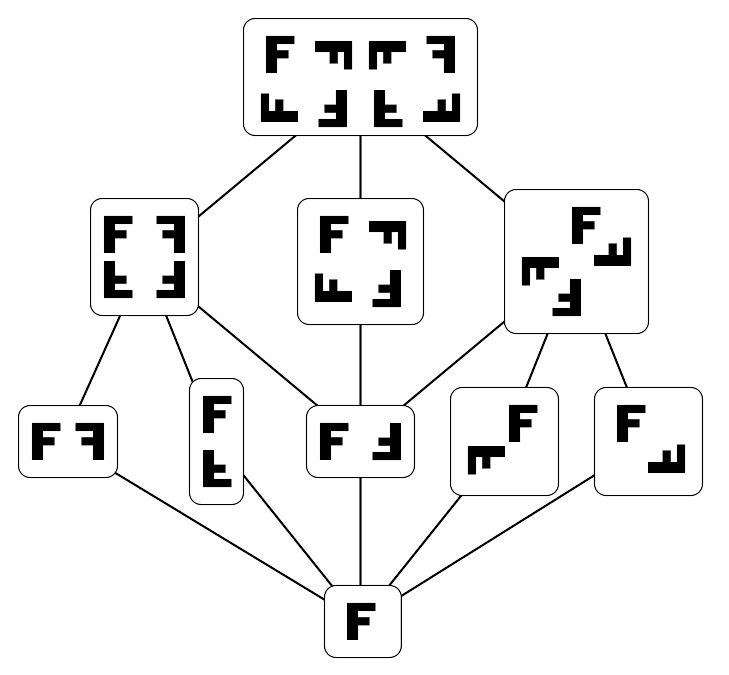
\includegraphics[width=0.25\textwidth]{reticulo-D4}
		\label{fig:reticuloD4dibujo}
		\caption{Retículo de subgrupos de $D_4$ de \cite{d4sub}}
	\end{figure}
	
	\textit{Nos ayudamos de la imágen para sacarlos. La manera de hacerlo sin tener más información que la presentación del grupo es hacerse todos los subgrupos generados por cada elemento y descartar los que son iguales. Luego hacerse todos los subgrupos generados por dos elementos y descartar los que son iguales. Por alguna razón no hace falta probar con los generados por más de dos elementos. Una vez obtenidos estos grupos establecemos las relaciones de inclusión y creamos el diagrama de Hasse.}
\end{ej}

\begin{ej}
	Retículo de subgrupos del grupo de cuaterniones $H$ (figura \ref{fig:reticulocuaterniones})
	
	\begin{figure}[h]
		\centering
		\begin{tikzpicture}
		\node (H) at (0,3) {$H$};
		\node (ab) at (-1.5, 2) {$\langle AB^2\rangle$};
		\node (a) at (0,2) {$\langle A \rangle$};
		\node (b) at (1.5,2) {$\langle B \rangle$};
		\node (b2) at (0,1) {$\{A^2 = B^2\}$};
		\node (e) at (0,0) {$\{e\}$};
		
		\draw (e) -- (b2) -- (a) -- (H);
		\draw (b2) -- (ab) -- (H);
		\draw (b2)-- (b) -- (H);
		\end{tikzpicture}
		\caption{Retículo de subgrupos del grupo de cuaterniones $H$.}
		\label{fig:reticulocuaterniones}
	\end{figure}

Para este ejemplo hemos probado con los posibles subgrupos que podían generar varios elementos.

\begin{itemize}
	\item Siempre se tiene que $\{e\} = \gen{1} < H$
	\item Además, como $H = \gen{A,B}$ tenemos por definición que $\gen{A} < H \land \gen{B} < H$.
	\item De calcular los órdenes de los elementos tenemos que el único con orden 2 es $B^2 = A^2$ por lo tanto su generado $\gen{B^2} = \{1, B^2\} < H$ (ver \autoref{ej:grupocuaterniones} para los órdenes).
	\item Cualquier grupo generado con una $A$ y una $B$ nos genera automáticamente todo $H$ por definición. Luego una posible estrategia es ver si algún otro elemento genera un subgrupo que no contenga a $A$ y a $B$.
	\begin{itemize}
		\item Nos damos cuenta después de muchas cuentas que $\gen{AB^2} = \{1, AB^2, A^2 = B^2, A\} < H$.
	\end{itemize}
\end{itemize}
\end{ej}

El retículo de subgrupos de $D_5$ lo veremos más adelante (para no llenar todo esto de retículos).

\begin{ej}
	
	Sea $G$ abeliano con $|G| = n = rs$, sea $H < G,\ K < G$ con $|H| = r,\ |K| = s$ y $H\cap K = \{e\}$.
	\begin{itemize}
		\item Notemos que como $G$ es abeliano, $H$ y $K$ son subgrupos normales.
		\item Al aplicar el teorema $\ref{thm:cardinalidadproductolibre}$ tenemos que el denominador es $|H\cap K| = 1$ por lo que $|HK| = |H| |K| = rs= n$.
		\item Como $G$ es abeliano:
		\begin{enumerate}
			\item $G = HK$ (porque $HK$ es un subgrupo con el mismo número de elementos que $G$ por el teorema \ref{thm:cardinalidadproductolibre})
			\item La función $f:H\times K \to G,\ (h, k)\mapsto hk$ es un homomorfismo de grupos (nótese que esto no ocurriría si $G$ no fuese abeliano).
		\end{enumerate}
	\end{itemize}
	
	Es más, si se cumple todo lo anterior, $f$ es además un isomorfismo $\implies H\times K \isom G$.
\end{ej}

\begin{ej}
	\label{ej:nohomoentreproducto}
	Consideramos $S_3$, que tiene $|S_3| = 6$ y no es abeliano y los subgrupos $H = \langle (12) \rangle$ y $K = \langle (123) \rangle$ con $|H| = 2$ y $|K| = 3$. Podemos construir la función $f:H\times K \to S_3$ pero no es un homomorfismo de grupos. De hecho, al ser $K \normsub S_3$, el producto $HK$ es un subgrupo y la función $f$ es una biyección, pero aún así no es compatible con la estructura de grupo.
\end{ej}

\begin{ej}
	Consideramos $D_4$ y un grupo $G$ con $a,b \in G$ donde hemos establecido un homomorfismo que definimos con $f(A) = a$ y $f(B) = b$. Ocurre lo siguiente
	\begin{itemize}
		\item El homomorfismo queda totalmente definido ya que todos los elementos de $D_4$ son palabras en $A$ y $B$ y por la estructura de homomorfismo podemos operar tras aplicar la operación a cada letra. Por ejemplo $f(ABA) = aba$.
		\item Es necesario que $o(a) = 2$ y $o(b) = 4$, de lo contrario no se cumpliría la estructura de homomorfismo entre $D_4$ y $G$.
	\end{itemize}
\end{ej}



\begin{ej}
	Veamos un ejemplo (notamos que $(12)^4 = id$)
	\begin{align*}
	f:\Z/4\Z &\to S_3 \\
	\overline{1} &\mapsto (12) \\
	\overline{2} &\mapsto id = (1) \\
	\overline{3} &\mapsto (12) \\
	\overline{4} = \overline{0} &\mapsto id
	\end{align*}
	
	Observamos que $\text{Hom}(\Z/4\Z, S_3) \subset \text{Hom}(\Z, S_3)$ puesto que al tomar $\Z/4\Z$ no podemos tomar cualquier $a$ sino que tenemos que asegurarnos de que $o(a) = o(1)$ (en este caso $o(a) = 2$ pero sigue funcionando porque lo que importa es que $a^{o(1)} = id$).
\end{ej}

Queremos analizar los homomorfismos $f:\ZnZ \to \ZnZ$. Ahora no importa el $\overline{a}$ que elijamos para que $f$ sea homomorfismo porque $\ima f = \langle \overline{a} \rangle$. 

Para que $f$ sea epimorfismo, necesitamos que $\ima f = \langle \overline{a} \rangle = \ZnZ$ es decir que $o(a)$ sea coprimo con $n$.

Concluímos que $\text{Aut}(\ZnZ) \subset \text{Hom}(\ZnZ, \ZnZ)$.



% !TeX root = ../apuntes-ea.tex

\chapter{El teorema de Cauchy}

\section{Consideraciones previas}

\subsection{Conjugación}

Cuando introdujimos los homomorfismos de grupos hicimos especial hincapié en un automorfismo al que llamábamos $\phi_g$ o $\gamma_g$ y que para un $g \in G$ dado se definía como
\begin{align*}
	\phi_g : G &\to G\\
			x &\mapsto gx\inv{g}
\end{align*}

Diremos a partir de ahora que dos elementos son conjugados si cumplen la siguiente definición.

\begin{dfn}[Conjugados]
	\label{dfn:elementosconjugados}
	Sea $G$ un grupo, $a,b \in G$. Diremos que $b$ es conjugado de $a \iff \exists g \in G \mid b = ga\inv{g}$, es decir, si existe un $g\in G$ para el que el automorfismo conjugación $\phi_g$ cumple $\phi_g(a) = b$.
\end{dfn}

Observemos que la conjugación es una relación de equivalencia.

\begin{pro}
	Sea $R$ una relación de equivalencia definida con
	\begin{align*}
		\forall a,b \in G,\quad aRb \iff \exists g \in G \mid b = ga\inv{g}
	\end{align*}
\end{pro}

Probamos las tres propiedades de las relaciones de equivalencia:
\begin{enumerate}
	\item Reflexiva: $\forall a \in G,\ aRa$
	\begin{proof}
		Tomando $g = e$ se tiene $\forall a, a = ea\inv{e} = eae = a$.
	\end{proof}
	\item Simétrica: $\forall a,b \in G,\ aRb \iff bRa$
	\begin{proof}
		Se verifica la doble implicación tomando $g' = \inv{g}$ utilizado en el otro lado:
		\begin{align*}
			aRb \implies \exists g \mid b = ga\inv{g} \iff \inv{g}bg = a \iff g' = \inv{g} \land a = gb\inv{g} \iff bRa
		\end{align*}
		Hacia el otro lado es igual.
	\end{proof}
	\item Transitiva: $\forall a,b,c \in G,\ aRb \land bRc \implies aRc$
	\begin{proof}
		\begin{align*}
		aRb \implies \exists g_1 \mid b = g_1a\inv{g_1} \qquad\land \qquad bRc \implies \exists g_2 \mid c = g_2b\inv{g_2} \\
		c = g_2b\inv{g_2} = g_2g_1a\inv{g_1}\inv{g_2} \implies c = g'a\inv{g'} \text{ con } g' = g_1 g_2 \implies aRc
		\end{align*}
	\end{proof}
\end{enumerate}

\textbf{Nota:} La relación de conjugación solo merece la pena en grupos no abelianos, porque en un grupo abeliano, cualquier par de elementos es conjugado.

\begin{ej}
	En $S_3$ afirmamos lo siguiente:
	\begin{itemize}
		\item que $1$ solo tiene como conjugado a sí mismo,
		\item que $\{(12),(13),(23)\}$ son conjugados entre sí,
		\item y que $\{(123),(132)\}$ también son conjugados entre sí.
	\end{itemize}
	Es decir, que la conjugación nos genera una partición con 3 cajas disjuntas.
\end{ej}

En esta relación de equivalencia, las clases de equivalencia son de la forma $cl(a) = \{ga\inv{g} \mid g \in G\}$ (conjuntos de los elementos que son conjugados de $a$). Queremos saber cuántos elementos hay en cada clase de equivalencia. Para ello introduciremos la noción de centralizador de un elemento y posteriormente daremos un teorema (\autoref{pro:cardinalcajas}) que relaciona el número de elementos del centralizador de un elemento con el número de elementos de la clase de equivalencia de un elemento.

%TODO: definición de clase de equivalencia por la relación de conjugación?


\subsection{Centro de un grupo}

\begin{dfn}[Centro de un grupo]
	\label{dfn:centro}
	Sea $G$ un grupo finito. Definimos el centro de $G$, $Z(G) = \{a \in G \mid \forall g \in G,\ ag = ga\}$.
\end{dfn}

El centro es útil en grupos finitos no abelianos ya que, en grupos abelianos, el centro es todo el grupo como veremos en la 
\autoref{pro:centroigualabeliano}.

\begin{pro}
	\label{pro:centrocerrado}
	Sean $a, b \in Z(G)$. Entonces $ab \in Z(G)$.
\end{pro}

\begin{proof}
	Tenemos que $ag = ga$ y que $bg = gb$. Ahora tenemos que probar que $g(ab) = (ab)g$. Es trivial manipulando $(ab)g = agb = gab$.
\end{proof}

\begin{pro}
	\label{pro:centronormal}
	Sea $G$ un grupo. $Z(G)$ es un subgrupo y además es un subgrupo normal.
\end{pro}

\begin{proof}
	Es un subgrupo porque es cerrado (ver \autoref{pro:centrocerrado}), contiene siempre al neutro (el centro conmuta con todos) y para todo $a \in Z(G)$, se tiene que $\forall b \in G,\ ab = ba \iff ab\inv{a} = b \iff b\inv{a} = \inv{a}b \iff \inv{a} \in Z(G)$.
	
	Es normal porque $\forall g \in G,\ Z(G)g = \{ag \mid a \in G \land \forall b \in G,\ ab = ba\} = \{ga \mid a \in G \land \forall b \in G,\ ab = ba\} = gZ(G)$.
\end{proof}

\begin{pro}
	\label{pro:subcentronormal}
	Si $H < Z(G)$ entonces $H$ es abeliano y normal.
\end{pro}

\begin{proof}
	Es abeliano porque $\forall g,g' \in Z(G),\ gg' = g'g$ y en particular esto se cumple para $g,g' \in G < G$.
	
	Es normal porque $\forall g \in G, gH = \{ga \mid a \in H \land \forall b \in G,\ gb = bg\} = \{ag \mid a \in G \land \forall b \in G,\ bg = gb\} = Hg$.
\end{proof}

\begin{pro}
	Sea $g \in G,\ \phi_g: G \to G$ el isomorfismo definido por $\phi_g(x) = gx\inv{g}$. Entonces
	\begin{align*}
	x \in Z(G) &\iff \forall g \in G, gx = xg \iff gx\inv{g} = x \\
	x \in Z(G) &\iff \forall g \in G,\ \phi_g(x) = x 
	\end{align*}
\end{pro}

\begin{pro}
	\label{pro:centroigualabeliano}
	$G$ es abeliano $\iff G = Z(G)$
\end{pro}

\begin{proof}
	Sea $a \in G \land o(a) = n$. Si $a$ es el único elemento de orden $n$ entonces $n = 2 \land a \in Z(G)$. Probamos primero que $n=2$. Si $a$ es el único elemento de orden $n$ entonces tiene que ocurrir que $a$ y $a^{n-1}$ tienen el mismo orden por lo que $1 = n-1 \implies n = 2$.
\end{proof}

La siguiente proposición es crucial para sacar conclusiones sobre los grupos sabiendo sobre sus órdenes y su centro.

\begin{pro}
	\label{pro:triplecentro}
	Si $G/Z(G)$ es cíclico de orden $n$ entonces $n = 1$. Otra manera de formularlo: Si $G/Z(G)$ es cíclico, entonces $G = Z(G)$. Otra manera más de formularlo: si $G/Z(G)$ es cíclico entonces $G$ es abeliano.
\end{pro}

\begin{proof}
	Supongamos que $G/Z(G) \isom \ZnZ$. Vamos a probar que $n$ tiene que ser 1. Supongmos que $G/Z(G) = \{\overline{\alpha_i}, i = 1, \dots, n\}$ donde $\overline{\alpha_i} = \alpha^i Z(G)$. Fijamos $g \in G$ con $g = \alpha^j h,\ h \in Z(G),\ 0 \leq j < n$ y fijamos $f' \in G$ con $g' = {\alpha^j}' h',\ h' \in Z(G),\ 0 \leq j' < n$. Entonces $gg' = \alpha^j h{\alpha^j}' h' = \alpha^{j+j'}hh' = {\alpha^j}' h' \alpha^j h = gg'$ (podemos conmutar las $h$ con cualquier elemento porque $h \in Z(G)$, por el contrario, los $\alpha$ no necesitamos conmutarlos, solo agruparlos cuando están juntos). Es decir, que $\forall g, g' \in G$ tenemos que $gg' = g'g$ por lo que $G$ es abeliano.
\end{proof}

\subsection{Centralizador de un elemento.}

\begin{dfn}[Centralizador de un elemento]
	\label{dfn:centralizador}
	Sea $a \in G$. Llamamos centralizador de $a$ al conjunto
	\begin{align}
	C(a) = \{g \in G \mid \gamma_g(a) = g a \inv{g} = a\}
	\end{align}
	Se tiene que $\forall a \in G,\ e \in C(a)$, es decir que $C(a)$ no es vacío.
\end{dfn}

\begin{pro}
	$a \in Z(G) \iff C(a) = G \iff [G:C(a)] = 1$
\end{pro}

\begin{proof}
	Es cristalina de las definiciones.
\end{proof}

\begin{pro}
	$C(a)$ es un subgrupo de $G$
\end{pro}

\begin{proof}
	Por el teorema \ref{thm:subconjuntocerrado} solo necesitamos probar la clausura, es decir, tenemos que probar que $\forall g,g' \in G,\ g \in C(a) \land g' \in C(a) \implies gg' \in C(a)$. Sale solo $(gg')a\inv{gg'} = gg'a\inv{(g')}\inv{g} = ga\inv{g} = a \in C(a)$.
\end{proof}

\begin{pro}
	\label{pro:cardinalcajas}
	$|cl(a)| = |\{ga\inv{g} \mid g \in G\}| = [G:C(a)]$ (el número de elementos de una clase de equivalencia es el índice del centralizador de un representante)
\end{pro}

De la proposición anterior se deduce que

\begin{cor}
	$|C(a)| = [G:cl(a)]$
\end{cor}

La prueba de la proposición se ve clara después de ver la prueba del teorema de Cauchy, así que la dejamos para después.


\section{Teorema de Cauchy}

\begin{thm}[de Cauchy]
	\label{thm:cauchy}
	Sea $G$ un grupo finito con $|G| = n$. Si $p$ es primo y $p\divides n$ entonces $G$ contiene un elemento de orden $p$.
\end{thm}

\begin{proof}
	Procedemos por casos:
	\begin{itemize}
		\item Si $G$ es abeliano. Descomponemos $|G| = n = p_1^{\alpha_1}p_2^{\alpha_2}\dots p_s^{\alpha_s}$. Por el teorema \ref{thm:noprobado1}, $G \isom \Z/p_1^{\beta_1}\Z \times \Z/p_2^{\beta_2}\Z \times \dots \times \Z/p_s^{\beta_r}\Z$ donde cada $\alpha_i$ es la suma de algunos $\beta_r \qed$.
		
		\item Si $G$ no es abeliano. Particionamos $G$ con la relación de equivalencia dada anteriormente (definición \ref{dfn:elementosconjugados}), $aRb \iff \exists g \in G \mid ga\inv{g} = b$. Recordemos que cada clase de equivalencia es de la forma $\overline{c} = \{gc\inv{g} \mid g \in G\}$. Observamos que si partimos de $e$, el elemento neutro, $eRb \implies \exists g \mid ge\inv{g} = b$ pero $\forall g \in G,\ ge\inv{g} = e$ por lo que $cl(e)$ tiene un único elemento.
		
		Tomemos ahora una clase de equivalencia, la que contenga a $a \in G$. La clase es $cl(a) = \{ga\inv{g} \mid g \in G\}$. Es claro que $a \in \overline{a}$ por la propiedad reflexiva de $R$, luego por lo menos en $cl(a)$ tiene un elemento.
		
		\begin{align*}
		cl(a) = \{ga\inv{g} \mid g \in G\} = \{a\} &\iff ga\inv{g} = a,\ \forall g \in G \\
		&\iff ga = ag,\ \forall g \in G
		\end{align*}
		\begin{align*}
		|cl(a)| = 1 &\iff \overline{a} = 1 \\
		&\iff a \in Z(G)
		\end{align*}
		
		Supongamos que la partición está dada por subconjuntos $cl(a_1), cl(a_2), \dots, cl(a_s)$. Por ser una partición, cualquier elemento vive en una sola caja, luego para saber cuantos elementos tiene $G$ nos vale con sumar los elementos de cada caja:
		\begin{align*}
		|G| = \sum_{i = 1}^{s} |cl(a_i)| = \sum_{i = 1}^n |\{ga_i\inv{g} \mid g \in G\}|
		\end{align*}
		Ahora bien, por la proposición \ref{pro:cardinalcajas} tenemos que $|cl(a_i)| = [G:C(a_i)]$. Por tanto decir que $|cl(a_i)| = 1 \implies [G:C(a_i)] = 1 \implies G = C(a_i)$.
		
		Ahora vamos a dividir el sumatorio en dos: por un lado las cajas de un solo elemento y luego las cajas de varios elementos:
		\begin{align}
		\label{eq:thmcauchy}
		|G| = |Z(G)| + \sum_{i = r + 1}^{s} [G : C(a_i)] \text{ donde } |Z(G)| = r \text{ y } [G : C(a_i)] \geq 2, \forall i = r+1,\dots, s
		\end{align}
		
		Ahora para probar el teorema de Cauchy procedemos por inducción en $n = |G| = [G:C(a_i)]\cdot |C(a_i)|$.
		
		\begin{enumerate}
			\item Caso $n = 1$. $G = \{e\}$ que es obvio.
			\item Caso $n = 2$. Son grupos cíclicos por lo que $\exists \alpha \in G \mid o(\alpha) = 2$.
			\item Caso $n \implies n+1$. Pueden pasar dos cosas:
			\begin{itemize}
				\item o bien $p \divides |C(a_i)|$ para algún $i = r+1, \dots, s$ entonces, por hipótesis inductiva, $C(a_i)$ contiene algún elemento de orden $p$. Pues ya está: $C(a_i) < G$ porque $\alpha \in C(a_i) \mid o(\alpha) = p \implies \alpha \in G$ también). \qedsymbol
				
				\item o bien $p \not\divides |C(a_i)|,\ \forall i = r+1,\dots,s$. No podemos proceder por inducción. Por hipótesis $|G| = [G:C(a_i)]\cdot |C(a_i)| \land p \divides |G| \implies p \divides [G: C(a_i)],\ \forall i = r+1,\dots, s$.
				
				Como $|G| = |Z(G)| + \sum_{i = r + 1}^{s} [G : C(a_i)]$ y por hipótesis $p \divides |G| \land p \divides [G : C(a_i)], \forall i = r+1,\dots,s \implies p \divides |Z(G)| \implies |Z(G)|$ es múltiplo de $p$. Como $Z(G)$ es abeliano, $\exists \alpha \in Z(G) \mid o(\alpha) = p$. Luego se reduce al caso abeliano y ya estaría \qedhere
			\end{itemize}
		\end{enumerate}
	\end{itemize}
\end{proof}

\begin{ej}
	Sea $G$ tal que $|G| = pq$. Entonces por le teorema de Cauchy $\exists a,b \in G \mid o(a) = p \land o(b) = q$. Como $p$ y $q$ son primos los ordenes de $\langle a \rangle$ y $\langle b \rangle$ son coprimos y por tanto $\langle a \rangle \cap \langle b \rangle = \{e\}$. Por el teorema del orden de conjunto producto libre (\ref{thm:cardinalidadproductolibre}), $|\gen{a} \gen{b}| = pq$. No sabemos si se tendrá que $G = \gen{a}\gen{b}$ ya que al no saber si alguno es normal, no podemos afirmar que el producto libre sea un grupo. Lo que si que sabemos es que $G = \{a^ib^j \mid 0 \leq i < p -1 \land 0 \leq j < q - 1\} = \langle a, b \rangle$.
\end{ej}

\begin{ej}
	Sea $G$ tal que $|G| = 2q$. Análogamente al caso anterior llegamos a que $o(a) = 2$. Como $\langle b \rangle$ tiene índice 2 entonces $\langle b \rangle \normsub G$. Esto nos permite saber como operar con las palabras $a^ib^j$ una vez tenemos un isomorfismo que lleva $a b \inv{a} = b^j$ (tiene que ir a algún $b^j$ porque por ser isomorfismo tiene que llevar elementos de orden $q$ en elementos de orden $q$: los $b \in \langle b \rangle$)
\end{ej}

Dada la relación de equivalencia de conjugación (definición \ref{dfn:elementosconjugados}), definimos $C$ como el conjunto de los representantes de las clases de equivalencia. Entonces podemos decir
\begin{align*}
G = \bigcup_{c_i \in C} \{a \in G \mid a R c_i\}
\end{align*}
Observemos que $d \in Z(G) \iff \{a \in G \mid a R d\} = \{gd\inv{g} \mid g \in G\} = \{d\}$. Y por tanto podemos escribir
\begin{align*}
C = Z(G) \cup (C\setminus Z(G))
\end{align*}
que aunque pareza obvio quiere decir que $C$ se puede expresar como la unión disjunta de las cajas que tienen solo un elemento que se corresponden con elementos que están en el centro y las cajas que tienen más de uno. Y por lo visto en la demostración del teorema de Cauchy tenemos que
\begin{align*}
|G| = \sum_{c_i \in C} | \overline{c_i} | = |Z(G)| + \sum_{i = r + 1}^{s} [G : C(a_i)] \text{ donde } [G : C(a_i)] \geq 2
\end{align*}

\subsection{P-grupos}

Una aplicación inmediata del teorema de Cauchy es la caracterización de los $p$-grupos.

\begin{dfn}[P-grupo]
	Sea $p$ primo. Decimos que $G$ es un p-grupo si $|G| = p^r$.
\end{dfn}

\begin{thm}
	Si $G$ es un p-grupo entonces $Z(G)$ es no trivial (no es el vacío).
\end{thm}

\begin{proof}
	Podemos escribir sin distinguir entre cajas de uno o varios elementos
	\begin{align*}
	|G| = |C(c_i)||[G:C(c_i)]|
	\end{align*}
	es decir que tenemos una factorización de $|G| = p^r$ luego $|C(c_i)|$ y $|[G:C(c_i)]|$ son ambos potencias de $p$. Y aplicando esto a la expresión \ref{eq:thmcauchy} tenemos que
	\begin{align*}
	\underbrace{|G|}_{\text{múltiplo de p}} = |Z(G)| + \sum_{i = r + 1}^{s} \underbrace{[G : C(a_i)]}_{\text{múltiplo de p}} \text{ donde } [G : C(a_i)] \geq 2
	\end{align*}
	por lo que $|Z(g)|$ tiene que ser múltiplo $p$ por lo que $Z(G)$ no puede ser el trivial.
\end{proof}

Véase un ejemplo de aplicación de esta anterior proposición en el ejercicio \nameref{ex:h2.22} y en el ejercicio \nameref{ex:h1.33}

\begin{ej}
	Tenemos que $Z(D_4) = \{1,B^2\}$ y $Z(H) = \{1, B^2\}$ donde $H$ es el grupo de cuateriones (\autoref{ej:grupocuaterniones}) y $D_4$ es el famoso grupo (\autoref{ej:famosogrupod4}).
\end{ej}

\begin{pro}
	\label{pro:primocuadradoabeliano}
	Si $p$ es primo y $|G| = p^2$ entonces $G$ es abeliano.
\end{pro}

\begin{proof}
	Por el la demostración del teorema anterior tenemos que o bien $|Z(G)| = p$ o bien $|Z(G)| = p^2$. Afirmamos que $|Z(G)| \neq p$ ya que si fuera así $|G/Z(G)| = p \implies G/Z(G)$ cíclico pero hemos probado (proposición \ref{pro:triplecentro}) que $G/Z(G)$ no puede ser cíclico. Por lo tanto $|Z(G)| = p^2 \implies Z(G) = G \implies G$ es abeliano.
\end{proof}


\section{Más sobre la conjugación, el centro y los centralizadores.}
Antes de introducir el teorema de Cauchy hablábamos de la conjugación que era una relación de equivalencia que partía un grupo $G$ en cajas. Nos gustaría saber cuántos elementos había en la clase de equivalencia de cada uno de los elementos de $G$ y para eso introducíamos el concepto de centralizador de un elemento: $C(a)$ el conjunto de los elementos de $G$ que no mueven a $a$ por conjugación. La \autoref{pro:cardinalcajas} nos aseguraba que $|cl(a)| = [G:C(a)]$ y dijimos que retrasaríamos la prueba hasta ahora. Pues aquí va.



Sea $\sim$ una relación de equivalencia definida por $a\sim b \iff \exists g \in G \mid ga\inv{g} = b$ para $a,b \in G$. Esta relación da una partición de $G$ en clases de la forma $cl(a) = \{ga\inv{g} \mid g \in G\}$. En el caso abeliano esta relación es la de igualdad, por lo que no nos merece la pena liar este pifostio para saber que $a\sim b \iff a = b$. 

Es muy importante saber cómo contamos los elementos de una clase, es decir, de cuantas formas podemos \textit{mover} el elemento $a$ con $g \in G$. Para ello definimos el centralizador (definición \ref{dfn:centralizador}) como $C(a) = \{h \in G \mid ha\inv{h} = a\} < G$. Queremos probar que $|cl(a)| = [G:C(a)] = r$.

\begin{proof}[Demostración de la \autoref{pro:cardinalcajas}]
	
	Lo probamos tomando clases laterales a la izquierda (por ejemplo) y partiendo $G$ en $r$ cajas. Las cajas son de la forma $\alpha_iC(a),\ i = 1, \dots, r$. Esta partición no tiene que ver con la partición anterior. Observemos que para cualquier $g \in \alpha_i C(a), g = \alpha_i h$, tenemos que $g a \inv{g} = \alpha_i h a \inv{h} \inv{\alpha_i} = \alpha_i a \inv{\alpha_i}$ es decir que los $g \in C(a)$ no se mueven fuera de la caja. Es decir, que si $\alpha_i \neq \alpha_j$ para $i\neq j$ entonces hay $r$ maneras de mover a $g$ y por tanto $|cl(a)| = r$.
	
	Probaremos que en efecto los $\alpha_i$ son distintos.
	
	Sean $g_1, g_2 \in G$. $g_1a\inv{g_1} = g_2a\inv{g_2} \iff (\inv{g_2}g_1)a(\inv{g_1}g_2) = a \iff (\inv{g_2}g_1)a\inv{(\inv{g_2}g_1)} \iff C(a) \inv{g_2}g_1 \in C(a) \iff g_1 \in g_2C(a)$.
	
	Si $G/\sim$ tiene $N$ elementos, tomamos $\{c_1, \dots, c_N\}$ como el conjunto de los representantes, donde $c_i$ es un representante de cada conjunto de la partición. Entonces pordemos expresar
	\begin{align*}
	G = \bigcup_{c_i \in C} = cl(c_i)
	\end{align*}
	donde $|cl(c_i)| = [G:C(c_i)]$. Por tanto decir que $|cl(c_i)| = 1$ es equivalente ($\iff$) a decir que $G = C(c_i) = \{\forall g \in G,\ gc\inv{g} = c\} \iff c \in Z(G)$.
	
	Afirmábamos que
	\begin{align*}
	|G| = \sum_{c_i \in C} |cl(c_i)| = |Z(G)| + \sum_{c_i \in C\setminus Z(G)} [G:C(c_i)]
	\end{align*}
	descomponiendo la suma en las clases con solo un elemento y las clases con más de dos elementos.
\end{proof}



\begin{ej}
	Consideramos $D_3$ (ver \autoref{ej:diedricosordengenerico}). Nos fijamos en que $B \not\in Z(D_3)$ es decir que en $cl(B)$ hay más de un elemento. En particular por lo visto anteriormente $|cl(B)| = [G:C(B)]$. Ahora bien $C(B) = \{1, B, B^2\}$ luego $|cl(B)| = [G:C(B)] = 2$. La pregunta es ¿quién es el compañero de $B$ en su clase? Es fácil, recordamos que $\phi_g (x) = gx\inv{g}$ (el isomorfismo conjugación) es un isomorfismo y que $\{1, B, B^2\}$ es normal, por lo que $o(B) = o(\phi_g(B)) = 2$. Entonces $\phi_g(B) \neq 1$ porque no coinciden los órdenes, de manera que $\phi_g(B) = B^2$ por necesidad. Luego el otro elemento es el $B^2$.
	
	¿Qué pasa con el elemento $A$? Pues ocurre que $A \in C(A)$ y $\{1, A\} \in C(A)$ y en realidad no puede haber más porque si hubiese un tercero, $\{1, A\}$ es un subgrupo de orden 2 $\implies o(\{1, A\})$ no divide a 3 $\implies$ si hubiese más, $C(A) = D_3$ y eso no puede ser $\implies C(A) = \{1, A\} \implies |cl(A)| = [D_3:C(A)] = 6/2 = 3$. Como las clases son disjuntas los tres elementos sobrantes forman la última caja.   
	
	Para conlcuir queda que la relación $\sim$ parte $D_3$ en 3 cajas, a saber:
	\begin{align*}
	D_3 = \{\underbrace{1}, \underbrace{B, B^2}, \underbrace{A, AB, AB^2}\}
	\end{align*}
\end{ej}


\begin{ej}
	\label{ej:clasesd4}
	El caso del famoso grupo $D_4$ (ver ejemplo \ref{ej:famosogrupod4})es mucho más interesante porque $Z(D_4)$ no es trivial. Elegimos por ejemplo el elemento $B^2$. Probar que $\phi_g(B^2) = gB^2\inv{g} = B^2,\ \forall g \in D_4$ es complicado. Pero fijémonos en que $\phi_B(B^2) = BB^2\inv{B} = B^2$ y que $\phi_A(B^2) = AB^2\inv{A} = B^2$. Entonces cualquier palabra en $A$ y en $B$ no mueve a $B^2$, por ejemplo $AB(B^2)\inv{B}\inv{A} = B^2$. Nos convencemos de que $B^2 \in Z(D_4)$. Con esto ya tenemos que $|Z(D_4)| \geq 2$ (puesto que de momento ya sabemos que $1, B^2 \in Z(G)$. Podría ser entonces $|Z(D_4)| = 4, 8$ (probamos los divisores de $|D_4|$). Como $D_4$ no es abeliano, es claro que $|Z(D_4) \neq 8$. Tampoco puede ser $|Z(D_4) \neq 4$ porque si tuviera 4, el cociente $D_4/Z(G)$ tendría orden $2$ y por tanto sería cíclico. Pero ya hemos probado que $G/Z(G)$ no puede ser cíclico (ver proposición \ref{pro:triplecentro}). Luego ya sabemos que $Z(D_4) = \{1, B^2\}$.
	
	Vamos a seguir sacando cajas. Veamos $cl(B)$. Claramente $B \in C(B)$ y por alguna razón que me falta $C(B) = \{1, B, B^2, B^3\}$. Por la fórmula tenemos que $|cl(B)| = [D_4:C(B)] = 2$. Tenemos una vez más que utilizar el isomorfismo de conjugación. Sabemos que $cl(B) = \{ga\inv{g} \mid g \in G\}$. Pero al ser $\phi_g$ isomorfismo y $\langle B \rangle$ normal, tenemos que $\phi_g : \langle b \rangle \to \langle b \rangle$ también es isomorfismo y por tanto lleva elementos de orden $n$ en elementos de orden $n$. Por tanto $\phi_g(B) = gB\inv{g}$ solo puede ser $B^3$ (a parte de $B$). Luego ya tenemos que $cl(B) = \{B, B^3\}$.
	
	¿Qué pasa con $A$? Pues es claro que $C(A) \supset \{1, A, B^2, AB^2\}$ ya que $B^2 \in Z(G)$ por lo que está en todos los $C(c_i)$.
	
	
	Segundo intento.
	
	\begin{enumerate}
		\item Como siempre $cl(e) = \{e\}$
		\item Veamos $cl(B)$. Queremos ver cuántos elementos tiene. Sabemos que $|cl(B)| = [D_4:C(B)]$. Veamos quién es $C(B)$. En primer lugar $B \in C(B) \implies \gen{B} \in C(B)$. Así ya tenemos que $|C(B)| \geq 4$. ¿Puede haber algún elemento más en $C(B)$? No, porque si hubiera uno más, su orden ya sería $|C(B)| = 8$ pues $C(B) < D_4$. Así concluímos que $|cl(B)| = [D_4:C(B)] = 8 / 4 = 2$. Además sabemos que $[D_4:C(B)] = 2 \implies C(B) \normsub D_4 \iff gC(B)\inv{g} = C(B) \forall g \in D_4 \implies gB\inv{g} \in C(B)$. Además como $gx\inv{g}$ es un isomorfismo que lleva elementos de orden $n$ en elementos de orden $n$ obtenemos que $o(gB\inv{g}) = o(B) = 2$. Sabemos que $B \in cl(B) \land cl(B) = \{gB\inv{g} \mid g \in D_4\} \land gB\inv{g} \in C(B) \implies gB\inv{g} = B^3$. Por tanto $cl(B) = \{B, B^3\}$.
		\item Veamos $cl(A)$. Queremos ver cuántos elementos tiene. Sabemos que $|cl(A)| = [D_4:C(A)]$. Veamos quién es $C(A)$. En primer lugar $A \in C(A) \implies \gen{A} \subset C(A)$. Si $B \in C(A)$ entonces $C(A) = G$ pues $B$ y $A$ generan. Esto no puede ser porque $C(A) = G \implies A$ conjuga con todos los demás elementos pero sabemos que $AB \neq BA$. Ocurre lo mismo con $B^3$. Probamos con $B^2$. $B^2AB^2 = BBAB^2 = BAB^3B^2 = BAB = AB^3B = A$ luego $B^2 \in C(A)$. Como $C(A) < D_4$ sabemos que es cerrado y por tanto $AB^2 \in C(A)$. Ya no puede haber más elementos porque si hubiera más, entonces $|C(A)| = 8$ y eso no puede ser. Por tanto $|cl(A)| = [D_4:C(A)] = 8 / 4 = 2$. Sabemos que $A \in cl(A)$. ¿Quién es el otro elemento? Como antes, $[D_4:C(A)] = 2 \implies C(A) \normsub D_4 \iff gC(A)\inv{g} = A$. Como $gx\inv{g}$ es un isomorfismo mantiene el orden y por tanto los conjugados de $A$ pueden ser $B^2$ o $AB^2$ (los únicos de orden 2 en $C(A)$
	\end{enumerate}
\end{ej}

\section{Normalizador de un subconjunto}

Vez pasada tomábamos $a \in G$ y teníamos $cl(a) = \{g a \inv{g} \mid g \in G\} = \{a=a_1, a_2, \dots, a_r\}$ y $C(a) = \{g \in G \mid ha\inv{h} = a \}$. Concluíamos que $|cl(a)| = [G:C(a)]$.

Vamos a generalizar al caso $S \subset G,\ S \neq \emptyset$. Consideramos la familia de subconjuntos siguiente:
\begin{align*}
\{gS\inv{g} \mid g \in G\} = \{S = S_1, S_2, \dots, S_r\}
\end{align*}
que tiene $r$ subconjuntos distintos.

Recordemos que la conjugación dada $\phi_g(x) = gx\inv{g}$ (el isomorfismo conjugación) es un isomorfismo\footnote{A veces tomate frito llama a este isomorfismo $\gamma_g$}, y por tanto una biyección entre subconjuntos $S_i \subset G$. Por tanto $|S| = \phi_g(S)$.

\begin{dfn}[Normalizador de un subconjunto]
	\label{dfn:normalizador}
	Fijado $S \subset G$, definimos el normalizador de $S$:
	\begin{align}
	N(S) = \{g \in G \mid gS\inv{g} = S\}
	\end{align} 
\end{dfn}

Se parece mucho a la definición de centralizador de un elemento (\autoref{dfn:centralizador}). En el caso en que $S = \{a\}$ tenemos que $N(S) = \{g \in G \mid ga\inv{g} = a\} = C(a)$.

Ojo, decir que $gS\inv{g} = S$ no significa que $\forall b_i \in S,\ gb_i\inv{g} = b_i$, sino que $gb_i\inv{g} \in S$ (no mandamos cada elemento a él mismo, sino que todos quedan dentro del subconjunto). Es decir que \textit{$N(S)$ es el conjunto de la totalidad de elementos para los que $\phi_g$ manda el subconjunto $S$ en sí mismo.}

\begin{pro}
	Dado $S \subset G,\ N(S)$ es un subgrupo.
\end{pro}

\begin{proof} Como $G$ es finito, $N(S)$ es subgrupo $\iff S \neq \emptyset \land N(S)$ es cerrado por la operación.
	\begin{itemize}
		\item Es claro que $e \in N(S)$ pues $eS\inv{e} = S$, luego $N(S) \neq \emptyset$.
		\item Tenemos que probar la clausura. Si $h_1S\inv{h_1} = S \land h_2S\inv{h_2} = S$ tenemos que $\underbrace{(h_2S\inv{h_2})}_{\in S}\inv{h_1} = S \implies h_1h_2 \in N(S)$.
	\end{itemize}
\end{proof}

\begin{pro}
	\label{pro:propiedad2Ns}
	$\{gS\inv{g} \mid g \in G\} = \{S = S_1, S_2, \dots, S_r\}$ son $r$ subconjuntos distintos. Es decir que $r = [G: N(S)]$.
\end{pro}

\begin{proof}
	A la izquierda del lector.\footnote{Left to the reader.}
\end{proof}

Supongamos ahora que en vez de ser $S \subset G$, tomamos $S < G$. Recordemos que dado $g\in G$, $\phi_g$ es un isomorfismo por tanto manda elementos de un subgrupo en otro subgrupo (si el subgrupo es normal, manda elementos de un subgrupo en sí mismo). Es por esto que la afirmación equivalente a la proposición anterior sería:

\begin{pro}
	Sea $S < G$. Entonces $\{gS\inv{g} \mid g \in G\} = \{S = S_1, S_2, \dots, S_r\}$ son $r$ subgrupos distintos.
\end{pro}

% TODO aquí había un teorema (el 3 de la página 80 de santorum que no hay quien lo entienda)

\begin{thm}
	Sea $G$ grupo, $H < G$. Entonces $H \normsub N(H)$ y $N(H)$ es el mayor subgrupo de $G$ con esta propiedad, es decir, $H \normsub H' \implies H' < N(H)$.
\end{thm}

\begin{proof}$ $\newline
	\begin{itemize}
		\item Para probar que $N\normsub N(H)$ tiene sentido olivdarse del grupo $G$. Tenemos que $h \in N(H) \iff hH\inv{h} = H, \forall h \in G$. En particular, tenemos que $hH\inv{h} = H,\ \forall h \in N(H) \implies H$ es normal en $N(H)$.
		
		\item Para porbar que $N(H)$ es el mayor subgrupo con esta propiedad demostraremos que si $H < H'$ y $H \normsub H'$ entonces $H' \subseteq N(H)$. La demostración es casi una tautología. Tenemos que $\forall h' \in H',\ h'H\inv{h'} = H \implies \forall h' \in H',\ h' \in N(H) \implies H' \subset N(H)$.
	\end{itemize}
\end{proof}

\begin{cor}
	$H \normsub G \iff N(H) = G$
\end{cor}

\begin{proof}
	Sabemos que $H\normsub H = \{gH\inv{g} \mid g \in G\}$ y dicho conjunto tiene $[G:N(H)] = 1$ elementos, luego $N(H) = G$. En otras palabras, el normalizador de un subgrupo $H < G$ normal es todo el grupo $G$.
\end{proof}

\begin{pro}
	Si $H < G$ entonces\footnote{No sé si la hipotesis aquí es que $H < G$ o que $H \subset G$} $Z(G) < N(H)$
\end{pro}

\begin{proof}
	Por definición de $Z(G)$ tenemos que los elementos $g \in Z(G)$ fijan no solo los elementos dentro de subconjuntos, sino que los fijan uno a uno. Por lo que es claro que $Z(G) < N(H)$. 
\end{proof}

\begin{pro}
	\label{pro:centralizadorsubgruponormalizador}
	Sea $g \in G$. Entonces $C(g) < N(\gen{g})$
\end{pro}

\begin{ej}
	Vamos a empezar por $G = S_3$. En $S_3$ tenemos los subgrupos $\langle (12) \rangle, \langle (13) \rangle, \langle (23) \rangle$ de orden 2 y el subgrupo $\langle (123) \rangle = \{(1), (123), (132)\}$ de orden 3.
	
	\begin{figure}[h]
		\centering
		\begin{tikzpicture}
			\node (neut) at (0,0) {$\{(1)\}$};
			\node (12) at (-2,1) {$\gen{(12)}$};
			\node (13) at (1, 1) {$\gen{(13)}$};
			\node (23) at (3,1) {$\gen{(23)}$};
			\node (123) at (-0.5,1.8) {$\gen{(123)}$};
			\node (s3) at (0,3.5) {$S_3$};
			
			\draw (neut) -- (12) -- (s3);
			\draw (neut) -- (23) -- (s3);
			\draw (neut) -- (13) -- (s3);
			\draw (neut) -- (123) -- (s3);
		\end{tikzpicture}
		\caption{Retículo de subgrupos de $S_3$}
		\label{fig:reticulos3}
	\end{figure}
	\begin{itemize}
		\item En el caso de este último $g\langle (123) \rangle \inv{g} = \langle (123) \rangle$ porque es el único subgrupo de orden 3. Por tanto $\langle (123) \rangle \normsub S_3$ y entonces $N(\langle (123) \rangle) = S_3$.
		\item Sin encambio en el caso de los subgrupos de orden $2$ es posible que $g\langle (12) \rangle \neq \langle (12) \rangle$, porque hay más de un subgrupo de orden 2. Observemos por ejemplo que $(13)(12)\inv{(13)} = (32) = (23)$, luego $\langle (12) \rangle$ no es normal en $S_3$, ya que hemos encontrado $g = (13) \in G$ que lo mueve. Pero ¿quién es el normalizador $N(\langle (12) \rangle)$? Pues ya sabemos que es un subgrupo propio, porque no puede dar todo $S_3$. Evidentemente $\langle (12) \rangle \subset N(\langle (12) \rangle)$. Luego tiene que ser que $N(\langle (12) \rangle) = \langle (12) \rangle$\footnote{No tiene gracia que $\langle (12) \rangle$ sea normal en sí mismo, lo que tiene gracia es que $\langle (12) \rangle$ es el mayor grupo donde $\langle (12) \rangle$ es normal.} 
	\end{itemize}
\end{ej}

%20181011

\begin{ej}
	Seguimos por \nameref{ej:famosogrupod4}). Vimos anteriormente (\autoref{ej:clasesd4}) que $Z(D_4) = \{1, B^2\}$. Tenemos su retículo en \autoref{fig:reticuloD4}. Queremos ver de entre los subgrupos de $D_4$, cuáles son los que conmutan.
	\begin{itemize}
		\item Empecemos por $\langle B \rangle = \{1, B, B^2, B^3\}$. Observamos que $\langle b \rangle$ es normal puesto que tiene índice 2, es decir que $\{g\langle B \rangle \inv{g} \mid g \in G\} = \{\langle B \rangle\}$ y tiene sentido que $[G:N(\langle B \rangle)] = 1$. Es decir que como $\langle B \rangle$ es normal tenemos que $N(\langle B \rangle) = D_4$.
		\item Seguimos por $H = \{1, A, B^2, AB^2\}$. Ocurre lo mismo, luego $N(H) = D_4$.
		\item Con el caso de $\langle B^2 \rangle$ tenemos también que $N(\langle B^2 \rangle) = D_4$ por ser normal.
		\item Agotados los subgrupos normales, nos quedan los más difíciles. Consideramos ahora $\langle A \rangle$. Una vez más nos preguntamos quién es el normalizador de $\langle A \rangle$.
		\begin{enumerate}
			\item Es claro que $\langle A \rangle$ conjugará con otros subgrupos de orden 2.
			\item También es claro que $\langle A \rangle \subset N(\langle A \rangle)$ y que $\langle B^2 \rangle \subset N(\langle A \rangle)$. Luego $N(\langle A \rangle)$ tiene al menos 2 elementos.
			\item También sabemos que $N(\langle A \rangle) \subsetneq G$ puesto que $\langle A \rangle$ no es normal, por lo que no puede tener 8 elementos. Por esto y porque $N(\langle A \rangle) < G$, concluimos que $|N(\langle A \rangle)| = 4$.
			\item ¿Cuáles mueven al $\langle A \rangle$? Sabemos que no puede haber más de dos, pues el normalizador tiene 4 elementos. Pues mirando la presentación nos damos cuenta de que $BA = A\inv{B} \iff BA\inv{B} = AB^2$. Luego nos damos cuenta de que $A$ se mueve a $AB^2$.
			\item Análogamente nos damos cuenta de que $AB$ se mueve a $AB^3$.
			\item Ya tenemos los dos elementos que se mueven.
		\end{enumerate}
	\end{itemize}
\end{ej}

\begin{ej}
	Vamos ahora con el grupo de cuaterniones $H$ descrito en el \autoref{ej:grupocuaterniones}.
	
	
	
	\begin{enumerate}
		\item Nos dibujamos el retículo. Se puede consultar en \autoref{fig:reticulocuaterniones}.
		\item Primeramente nos damos cuenta de que $\langle A \rangle \cap \langle b \rangle \supsetneq \{e\}$ porque $H$ tiene 8 elementos y por la fórmula del producto libre (\autoref{thm:cardinalidadproductolibre}) y porque todo producto directo de subgrupos está contenido en el grupo aunque no sea subgrupo.
		\item Ocurre lo mismo con los demás subgrupos de orden 4 ($\langle A \rangle,\ \langle AB \rangle$). Tiene que tener intersección no vacía. En concreto la intersección es el subgrupo generado $\langle A^2 = B^2 = (AB)^2 \rangle$.
		\item En $H$ todos los subgrupos son normales, por lo que no tienen "órbitas" de modo que es muy aburrido.
	\end{enumerate}
\end{ej}

\begin{ej}
	Consideramos ahora $D_5$ que funciona como el $D_4$ (ver \autoref{ej:diedricosordengenerico} para más información sobre los grupos $D_n$).
	\begin{figure}[h]
		\centering
		\begin{tikzpicture}
		\node (d5) at (0,2) {$D_5$};
		\node (a) at (-3.75, 1) {$\langle A \rangle$};
		\node (ab) at (-2.25, 1) {$\langle AB \rangle$};
		\node (ab2) at (-0.75, 1) {$\langle AB^2 \rangle$};
		\node (ab3) at (0.75, 1) {$\langle AB^3\rangle$};
		\node (ab4) at (2.25, 1) {$\langle AB^4\rangle$};
		\node (b) at (3.75, 1) {$\langle B \rangle$};
		\node (e) at (0,0) {$\{1\}$};
		
		\draw (e) -- (a)   -- (d5);
		\draw (e) -- (ab)  -- (d5);
		\draw (e) -- (ab2) -- (d5);
		\draw (e) -- (ab3) -- (d5);
		\draw (e) -- (ab4) -- (d5);
		\draw (e) -- (b)   -- (d5);
		\end{tikzpicture}
		\caption{Retículo de subgrupos de $D_5$.}
		\label{ej:reticulod5}
	\end{figure}

	\begin{itemize}
		\item Primera observación. Como $o(B) = 5$ que es primo, tenemos que $o(B^k) = 5,\ k = 1, \dots, 4$. Luego cualquier subgrupo generado por $\langle B^k \rangle = \langle B \rangle$. Aquí falta algo. % TODO revisar este ejemplo que está en la página 85 de santorum
		\item Observemos que los subgrupos propios pueden ser de 2 o 5 elementos.
		\item No puede haber subgrupos generados por dos elementos de $D_5$ (por qué?)
		\item Los únicos subgrupos son $\langle B \rangle$ y los generados por $A, AB, AB^2, AB^3, AB^4$.
		\item Afirmamos que $\{gA\inv{g} \mid g \in G\} = \{\langle A \rangle, \langle AB \rangle, \langle AB^2 \rangle, \langle AB^3 \rangle, \langle AB^4 \rangle \}$. Vamos a probarlo.
		
		\begin{enumerate}
			\item Primero nos damos cuenta de que $\{1, A\} \in N(\langle A \rangle)$.
			\item Además tenemos que no puede haber otro grupo por encima de $\langle A \rangle$ y $D_5$ por lo que tenemos que $N(A) = \langle A \rangle$.
			\item Por tanto en la órbita de $A$ tenemos $[D_5:\langle A \rangle] = 5$ grupos.
		\end{enumerate}
		
	\end{itemize}
\end{ej}


% !TeX root = ../apuntes-ea.tex

\chapter{Biyecciones}

\section{El por qué de la notación cíclica}

\begin{dfn}[Conjunto de biyecciones]
	Sea $X$ un conjunto. Definimos
	\begin{align*}
		\biy{X} = \{f: X \to X \mid f \text{ es biyección}\}
	\end{align*}
\end{dfn}

Como coinciden dominio y codominio ($f:X \to X$) si $f$ es inyectiva entonces automáticamente es sobre y por tanto biyectiva.

En general, tiene sentido pensar en $Biy(X)$ aunque $|X| = \infty$. Además, en dicho conjunto viven la biyección identidad y la biyección inversa para cada biyección. Por tanto, tiene sentido pensar en $(Biy(X), \circ)$ como un grupo (la composición de biyecciones da una biyección). Lo escribimos en forma de teorema.

\begin{thm}
	Sea $X$ un conjunto. El par $(\biy{X}, \circ)$ es un grupo.
\end{thm}

Nos concentraremos en el caso en el que $|X| = n < \infty$ que nos da $Biy(X) = S_n$. Ver \autoref{dfn:sn} para una explicación detallada del grupo $S_n$.

Fijamos un conjunto $X$ y un homomorfismo de grupos $\alpha: X \to Biy(X)$. A partir de estos datos definimos una relación de equivalencia que nos da una partición de $X$, es decir, vamos a partir $X$ en conjuntos disjuntos. Veamos un ejemplo particular.

\begin{ej}
	Supongamos $G = X,\ |G| = n$ y consideramos $\rho: G \to \autom{G} \subset Biy(X)$. Definimos la relación en $X = G$
	\begin{align*}
	aRb \iff \exists g \in G \mid \phi_g(a) = b,\ \phi_g(x) = gx\inv{g}
	\end{align*}
	que es la relación de conjugación dada por el isomorfismo de conjugación de toda la vida.
	
	Ahora, en lugar de pensar en $G = X$ pensamos en $X = \{H < G\}$ (los subgrupos de $G$). Para cualquier isomorfismo de grupos $\beta: G \to G$, tenemos que si $H < G$ entonces $\beta(H) < G$.
	
	Lo que hemos hecho aquí es un caso particular de lo que viene ahora.
\end{ej}

Ahora pasamos al caso general.

\begin{pro}
	Sea $\alpha: G \to Biy(X),\ g \mapsto \alpha(g)$ un homomorfismo de grupos\footnote{Ojo: aquí las imágenes de los elementos $g \in G$ son biyecciones $f:G \to G$, por eso tendrá sentido la notación $\alpha(g)(a)$ que significa aplicar la función que nos devuelve $\alpha$ al elemento $a \in G$.}. Definimos la relación de equivalencia $R$ en el conjunto $X$
	\begin{align}
	aRb \iff \exists g \in G \mid \alpha(g)(a) = b
	\end{align}
	Afirmamos que la relación es de equivalencia y que nos divide $X$ en subconjuntos disjuntos (nos particiona $X$).
\end{pro}

\begin{proof}Probamos las 3 propiedades de las relaciones de equivalencia.
	\begin{enumerate}
		\item Reflexiva: $\forall x \in X, a R a$. Por ser $\alpha$ homomorfismo tenemos que $\alpha(e_G) = id_X$ y por tanto $\alpha(e_G)(a) = a$.
		\item Simétrica: $aRb \implies bRa$. Partimos de que $\exists g \in G \mid \alpha(g)(a) = b$. Tomamos $\inv{g} \in G$ y por ser $\alpha$ homomorfismo de grupos tenemos que $\alpha(\inv{g})(b) = \inv{(\alpha(g))}(b) = a$.
		\item Transitiva: $aRb \land bRc \implies aRc$. Partimos de que $\exists g, g' \in G \mid \alpha(g)(a) = b \land \alpha(g')(b) = c$. Tomamos $g'g \in C$ y tenemos que $\alpha(g'g)(a) = \alpha(g')(\alpha(g)(a)) = \alpha(g')(b) = c$ por composición de biyecciones.
	\end{enumerate}
\end{proof}

¿Cómo son las clases que da la partición?

Pues tenemos que para $a \in X$, la clase $cl(a) = \{\alpha(g)(a) \mid g \in G\}$. Definimos $H_a = \{g \in G \mid \alpha(g)(a) = a\}$. Tenemos por lo visto anteriormente que $H_a < G \land |cl(a)| = [G:H_a]$. Entonces tenemos lo siguiente:
\begin{itemize}
	\item En el caso en que $X = G$, es decir, que el conjunto $X$ tiene dentro \textit{elementos} de $G$, tenemos que $H_a = C(a)$ donde $C(a)$ es el centralizador de $a$ (\autoref{dfn:centralizador}).
	\item En el caso en que $X = \{H < G\}$, es decir, que el conjunto $X$ tiene dentro \textit{subgrupos} de $G$, tenemos que $H_a = N(a)$ donde $N(a)$ es el normalizador de $a$ (\autoref{dfn:normalizador}).
\end{itemize}

Vista la definición abstracta, lo que nos interesa de esto es aplicarlo a los grupos $S_n$ de los que hablábamos antes. En particular, ahora daremos una definición formal de ciclo para la notación que introdujimos en la \autoref{sec:notacionciclica}.

\begin{wrapfigure}{l}{0.3\textwidth}
	\begin{tikzpicture}
	\begin{scope}[scale=0.5]
	\node (alpha) at (-2, 0) {$\alpha :=$};
	\node (1) at (0,4) {$1$};
	\node (2) at (0,3) {$2$};
	\node (3) at (0,2) {$3$};
	\node (4) at (0,1) {$4$};
	\node (dots) at (0,-1) {$\vdots$};
	\node (nmenos1) at (0,-2) {$n-1$};
	\node (n) at (0,-3) {$n$};
	
	\node (1p) at (6,4) {$1$};
	\node (2p) at (6,3) {$2$};
	\node (3p) at (6,2) {$3$};
	\node (4p) at (6,1) {$4$};
	\node (5p) at (6,0) {$5$};
	\node (dotsp) at (6,-1) {$\vdots$};
	\node (nmenos1p) at (6,-2) {$n-1$};
	\node (np) at (6,-3) {$n$};
	
	\node (dotsc) at (3, -1) {$\vdots$};
	
	
	\draw (1) -- (2p);
	\draw (2) -- (1p);
	\draw (3) -- (4p);
	\draw (4) -- (5p);
	\draw (nmenos1) -- (np);
	\draw (n) -- (3p);
	\end{scope}
	\end{tikzpicture}
	\caption{La permutación $\alpha$ de $S_n$}
	\label{fig:permalphaejpart}
\end{wrapfigure}

Fijamos $\sigma \in S_n$ y definimos $G = \gen{\sigma}$ el subgrupo generado por $\sigma$ en $S_n$. Definimos ahora el homomorfismo
\begin{align*}
G = \gen{\sigma} & \to S_n = \biy{X},\qquad X = \{1, 2, 3, \dots, n\}
\end{align*}
Las clases $cl(i)$ para $i \in \{1, 2, \dots, n\}$ son de la forma\footnote{Las clases serían de la forma $\alpha(g)(i)$ pero es que en este caso todos los $\alpha(g)$ son elementos de $G = \gen{\sigma}$ y por tanto son de la forma $\sigma^k$.}
\begin{align*}
cl(i) = \{\sigma^k(i) \mid k \in \Z\}
\end{align*}


\begin{ej}
	Consideramos la permutación $\alpha \in S_n$ dada por (ver \autoref{fig:permalphaejpart})
	\begin{align*}
		\alpha = \begin{array}{ccccccc}
		1 & 2 & 3 & 4 & \dots & n-1 & n \\
		2 & 1 & 4 & 5 & \dots & n & 3
		\end{array}
	\end{align*}
	que en la notación cíclica podríamos escribir como $\alpha = (345\dots n)(12)$.
	
	En este caso la clase $cl(1) = \{1, 2\} = cl(2)$ está formada por los elementos que podemos obtener de aplicar $\alpha$ al elemento $1$. Ya se intuye la utilidad de la notación cíclica: la permutación $\alpha$ nunca mezcla elementos de la caja $\{1,2\}$ con elementos de la caja $\{3, 4, 5, \dots, n\}$. Así, también tendremos que $cl(3) = cl(4) = \dots = cl(n) = \{3, 4, 5, \dots, n\}$. Los elementos que hay en estas dos clases coinciden con los elementos que hay en cada uno de los ciclos en los que hemos descompuesto $\alpha$.
\end{ej}

Vemos que si fijamos $\sigma$ se define una partición en $\{1, \dots, n\}$ de subconjuntos disjuntos
\begin{align*}
F_1 \cup F_2 \cup \dots \cup F_n
\end{align*}

Si $r = |F_i| > 1$, $F_i = \{i_0, i_1, \dots, i_r\}$ tal que $\sigma(i_0) = i_1, \sigma(i_1) = i_2, \dots, \sigma(i_r) = i_0$.

\begin{dfn}[Ciclo]
	\label{dfn:ciclo}
	Diremos que $\sigma$ es un ciclo de longitud $r$ si en la partición definida
	\begin{align*}
	F_1 \cup F_2 \cup \dots \cup F_n
	\end{align*}
	todas las cajas $F_j,\ j < r$ tienen un único elemento y $F_r$ tiene $r$ elementos.
\end{dfn}

La definición quiere decir que, en el fondo, un ciclo es un tipo de permutación que al aplicarla sucesivamente sobre el conjunto $X$ lo particiona en varias cajas pero de manera que todas tienen un elemento excepto una, que tiene todos los elementos que se mueven entre ellos por la acción del ciclo. Un ejemplo en el conjunto $X = \{1, 2, 3, \dots, n\}$ sería

\begin{center}
	\begin{tabular}{|c|c|c|c|}
		\hline
		1 & 5 & \dots & \vdots \\\cline{2-4}
		2 & 6 & $\ddots$ & \vdots \\\cline{2-4}
		3 & $\ddots$ & $\ddots$ & \vdots  \\\cline{2-4}
		4 & \dots & \dots & n\\\hline
	\end{tabular}
\end{center}

Observemos que por la notación que hemos elegido, los ciclos tienen la estructura $(\sigma^0(a)\ \sigma^1(a)\ \sigma^2(a) \dots \sigma^s(a))$ donde $\sigma$ es un elemento de $S_n$ y $a$ un elemento de $X$. Dado que si $\sigma^k = Id$ entonces $\sigma^{k + i} = \sigma^i$, si \textit{rotamos} los números que definen el ciclo no estamos haciendo nada. Esto es, el ciclo $(1234) = (2341) = (3412) = (4123)$.

\section{De permutaciones a composiciones de ciclos}

\begin{pro}
	Toda biyección $\alpha \in S_n$ se puede expresar como composición de ciclos disjuntos dos a dos:
	\begin{align*}
		\alpha = \sigma_1 \circ \sigma_2 \circ \dots \circ \sigma_s
	\end{align*}
\end{pro}

\begin{pro}
	La composición de dos ciclos disjuntos conmuta, es decir, si $\sigma_1$ y $\sigma_2$ son ciclos disjuntos (que no comparten ningún elemento entre los paréntesis) entonces $\sigma_1 \circ \sigma_2 = \sigma_2 \circ \sigma_1$
\end{pro}

\begin{cor}
	Toda descomposición de una permutación $\alpha \in S_n$ en ciclos disjuntos $\alpha = \sigma_s \circ \sigma_{s-1} \circ \dots \circ \sigma_2 \circ \sigma_1$ se puede reordenar sin cambiar el resultado.
\end{cor}

\begin{ej}
	Antes de seguir veamos un ejemplo más de cómo una biyección de $S_n$ particiona el conjunto $X = \{1, 2, \dots, n\}$.
	
	Consideramos $\alpha \in S_n$ definida con
	\begin{align*}
		\alpha = \left(\begin{array}{cccccccccc}
		1 & 2 & 3 & 4 & 5 & 6 & 7 & 8 & 9 & 10 \\
		2 & 3 & 1 & 5 & 6 & 4 & 7 & 9 & 8 & 10
		\end{array}\right)
	\end{align*}
	
	La partición que nos da $\alpha$ de $X = \{1, 2, 3, 4, 5, 6, 7, 8, 9 10\}$ es la siguiente:
	\begin{center}
		\begin{tabular}{|c|c|c|c|}
			\hline
			1 & 4 & 7 & \\ \cline{3-3}
			2 & 5 & 8 & 10 \\
			3 & 6 & 9 & \\
			\hline
		\end{tabular}
	
		Partición de $X$ dada por $\alpha = (123)(456)(89)$
	\end{center}
	Esto lo obtenemos de buscar las clases de cada elemento. Empezamos por el que queramos, por ejemplo, el $1$:
	\begin{align*}
		cl(1) = \{\alpha^k(1) \mid k \in \Z\} = \{\alpha^0(1) = 1, \alpha^1(1) = 2, \alpha^2(1) = 3, \alpha^3(1) = 1, \alpha^4(1) = 2, \dots \}
	\end{align*}
	Eliminando duplicidades obtenemos que $cl(1) = \{1,2,3\}$. Análogamente obtenemos $cl(4) = \{4,5,6\},\ cl(7) = \{7\},\ cl(8) = \{8,9\},\ cl(10) = \{10\}$. Lo que hemos hecho es seguir el algoritmo descrito en la \autoref{sec:notacionciclica}, esta vez entendiendo el significado. Obtenemos que $\alpha = (123)(456)(89)$ o cualquier reordenación de los ciclos anteriores, ya que al ser disjuntos, cambiar el orden en el que los rotamos no afecta al resultado.
\end{ej}

\begin{wrapfigure}{l}{0.3\textwidth}
	\centering
	\begin{tikzpicture}
	\node (1) at (0,1) {${1}$};
	\node (2) at (0.866,0.5) {$2$};
	\node (3) at (0.866,-0.5) {$3$};
	\node (4) at (0, -1) {$4$};
	\node (5) at (-0.866, -0.5) {$5$};
	\node (6) at (-0.866,0.5) {$6$};
	
	\draw[->] 	(1) edge (2)
	(2) edge (3)
	(3) edge (4)
	(4) edge (5)
	(5) edge (6)
	(6) edge (1);
	\end{tikzpicture}
	\caption{El ciclo $\sigma = (123456)$}
	\label{fig:ciclo16}
	
	
	\begin{tikzpicture}
	\node (1) at (0,1) {${1}$};
	\node (2) at (0.866,0.5) {$2$};
	\node (3) at (0.866,-0.5) {$3$};
	\node (4) at (0, -1) {$4$};
	\node (5) at (-0.866, -0.5) {$5$};
	\node (6) at (-0.866,0.5) {$6$};
	
	\draw[->] 	(1) edge (3)
	(3) edge (5)
	(5) edge (1)
	(2) edge (4)
	(4) edge (6)
	(6) edge (2);
	\end{tikzpicture}
	\caption{El ciclo $\sigma^2 = (123456)^2$}
	\label{fig:ciclo16cuadrado}
	
	\begin{tikzpicture}
	\node (1) at (0,1) {${1}$};
	\node (2) at (0.866,0.5) {$2$};
	\node (3) at (0.866,-0.5) {$3$};
	\node (4) at (0, -1) {$4$};
	\node (5) at (-0.866, -0.5) {$5$};
	\node (6) at (-0.866,0.5) {$6$};
	
	\draw[->] 	(1) edge[bend left] (4)
	(4) edge[bend left] (1)
	(2) edge[bend left] (5)
	(5) edge[bend left] (2)
	(3) edge[bend left] (6)
	(6) edge[bend left] (3);
	\end{tikzpicture}
	\caption{El ciclo $\sigma^3 = (123456)^3$}
	\label{fig:ciclo16cubo}
\end{wrapfigure}

Veamos ahora cómo se relacionan los órdenes de los ciclos con su longitud.


\begin{ej}
	Consideramos $\sigma = (123456) \in \S_n$. Observamos que $\sigma^6 = Id$ es decir que $\sigma$ tiene orden 6.
	
	De esta manera si nos preguntan por $\sigma^{122} = (123456)^{122} = (123456)^{6\cdot20} \circ (123456)^2 = (123456)^2$ no nos asustamos.
	
	Si nos hubieran dado $\sigma$ con la notación habitual, aparte de que hubiera ocupado mucho, no podríamos haber resuelto esta operación tan rápido.
\end{ej}


\begin{ej}
	Nos preguntamos ahora por las potencias de $\sigma = (123456)$ menores que $6 = o(\sigma)$.
	\begin{itemize}
		\item $\sigma^2$ equivaldría a aplicar $\sigma$ dos veces a cada número $\{1, \dots, 6\}$ (los demás números no nos interesan porque sabemos que $\sigma$ no los mueve). Ayudándonos del dibujo obtenemos que $\sigma^2 = (135)(246)$.
		
		Se verifica que $\sigma^2$ tiene $o(\sigma^2) = 3$ y además si recordamos el \autoref{thm:ordendepotencia} comprobamos que se verifica $o(\sigma^2) = \frac{o(\sigma)}{mcd(o(\sigma), 2)} = \frac{6}{2} = 3$.
		
		\item En cuanto a $\sigma^3$ observamos que al aplicar $\sigma$ 3 veces nos quedan 3 ciclos y que se vuelve a verificar que $o(\sigma^3) =\frac{o(\sigma)}{mcd(o(\sigma), 3)} = \frac{6}{3} = 2$
	\end{itemize}
\end{ej}

Esto nos lleva a enunciar el siguiente teorema

\begin{thm}
	\label{thm:ordenpotenciasciclos}
	Sea $\sigma = (i_1\ i_2\ i_3 \dots i_n)$ un ciclo de longitud $n$. Sea $m \in \Z$ y $d = mcd(n,m)$. Entonces $\sigma^m$ es un producto de $d$ ciclos de longitud $\frac{n}{d}$ y estos son disjuntos dos a dos.
\end{thm}

Poder averiguar los órdenes de ciclos es una herramienta muy potente. Por ejemplo, podemos hacer lo siguiente.

\begin{ex}[H3.8]
	Demuestra que el subgrupo $G < S_4$ generado por los elementos $\sigma = (1432)$ y $\tau = (24)$ es isomorfo a $D_4$.
\end{ex}

\begin{proof}
	Sabemos que $o(\sigma) = 4$ y que $o(\tau) = 2$. Trabajando un poco vemos que
	\begin{align*}
		\gen{\sigma} &= \{\sigma = (1432), \sigma^2 = (13)(24), \sigma^3 = (4321), \sigma^4 = Id\} \\
		\gen{\tau} &= \{\tau = (24), \tau^2 = Id\}
	\end{align*}
	Faltaría ver que $\sigma \tau = \tau \sigma^3$ es decir que $(1432)(24) = (24)(4321)$ (spoiler: es verdad) y ya podríamos identificar $\sigma$ con $B$ y $\tau$ con $A$ para obtener la presentación del famoso grupo $D_4$:
	\begin{align*}
		D_4 \isom G = \gen{\sigma, \tau \mid o(\sigma) = 4 \land o(\tau) = 2 \land \sigma \tau = \tau \sigma^3}
	\end{align*}
\end{proof}

\begin{thm}
	Sea $\alpha$ una permutación expresada como composición de ciclos disjuntos $\alpha = \sigma_1 \circ \sigma_2 \circ \dots \circ \sigma_n$. Entonces el orden de $\alpha$ es el mínimo común múltiplo de los órdenes de cada $\sigma_i$:
	\begin{align*}
		\alpha = \sigma_1 \circ \sigma_2 \circ \dots \circ \sigma_n \text{ disjuntos } \implies o(\alpha) = mcm(\sigma_1, \dots, \sigma_n)
	\end{align*}
\end{thm}

% TODO demostrar esto: dorronsoro página 120

\begin{proof}
	Ver \cite[p.~120]{dor96}.
\end{proof}

\section{Sobre las conjugaciones de una descomposición en ciclos}

Antes de seguir, vamos a introducir dos proposiciones que nos serán de gran ayuda al calcular conjugados de una permutación, por ejemplo, para cuando queramos calcular centralizadores.

\begin{pro}
	Sea $\alpha \in S_n$ una permutación con descomposición en ciclos disjuntos
	\begin{align*}
	\alpha = \left(i_1^{(1)}\ i_2^{(1)}\ \dots\ i_{s_1}^{(1)}\right)\left(i_1^{(2)}\ i_2^{(2)}\ \dots\ i_{s_2}^{(2)}\right)\dots\left(i_1^{(r)}\ i_2^{(r)}\ \dots\ i_{s_r}^{(r)}\right)
	\end{align*}
	y sea $\omega \in S_n$. Entonces el conjugado de $\alpha$ por $\omega$ es $\alpha'$ y se obtiene de
	\begin{align*}
	\alpha' = \omega \alpha \inv{\omega} = \left(\omega(i_1^{(1)})\ \omega(i_2^{(1)})\ \dots\ \omega(i_{s_1}^{(1)})\right)\left(\omega(i_1^{(2)})\ \omega(i_2^{(2)})\ \dots\ \omega(i_{s_2}^{(2)})\right)\dots\left(\omega(i_1^{(r)})\ \omega(i_2^{(r)})\ \dots\ \omega(i_{s_r}^{(r)})\right)
	\end{align*}
\end{pro}

Se ve mejor con un ejemplo:

\begin{ej}
	Sea $\alpha = (123)(45) \in S_5$ y sea $\omega \in S_5$ alguna permutación. Entonces
	\begin{align*}
	\alpha' = \omega\alpha\inv{\omega} = \omega(123)(45)\inv{\omega}= \left(\omega(1)\ \omega(2)\ \omega(3)\right)\left(\omega(4) \omega(5)\right)
	\end{align*}
\end{ej}

También podemos ir en la otra dirección. Es decir, dados $\alpha$ y $\alpha'$ obtener $\omega$:

\begin{pro}
	Sean $\alpha, \alpha' \in S_n$ dos permutaciones cuyas descomposiciones en ciclos disjuntos son del mismo tipo y se denotan por
	\begin{align*}
	\alpha = \left(i_1^{(1)}\ i_2^{(1)}\ \dots\ i_{s_1}^{(1)}\right)\dots\left(i_1^{(r)}\ i_2^{(r)}\ \dots\ i_{s_r}^{(r)}\right) \\
	\alpha' = \left(j_1^{(1)}\ j_2^{(1)}\ \dots\ j_{s_1}^{(1)}\right)\dots\left(j_1^{(r)}\ j_2^{(r)}\ \dots\ j_{s_r}^{(r)}\right)
	\end{align*}
	Entonces $\exists \omega \in S_n$ tal que $\alpha' = \omega \alpha \inv{\omega}$ y $\omega$ se puede construir (en notación no cíclica)
	\begin{align*}
	\omega = \left(\begin{array}{ccccccccc}
	i_1^{(1)}\ &i_2^{(1)}\ &\dots\ &i_{s_1}^{(1)}\ & \dots\ &i_1^{(r)}\ &i_2^{(r)}\ &\dots\ &i_{s_r}^{(r)} \\
	j_1^{(1)}\ &j_2^{(1)}\ &\dots\ &j_{s_1}^{(1)}\ & \dots\ &j_1^{(r)}\ &j_2^{(r)}\ &\dots\ &j_{s_r}^{(r)}
	\end{array}\right)
	\end{align*}
\end{pro}

\begin{ej}
	Sean $\sigma, \sigma' \in S_5$. Busco $\tau \in S_5$ tal que $\sigma'$ sea conjugada de $\sigma$ por $\tau$, es decir, $\tau \in S_n \mid \sigma' = \tau\sigma\inv{\tau}$. Pues utilizamos el método
	\begin{align*}
	\begin{cases}
	\sigma 	&= (123)(45) \\
	\sigma' &= (245)(13)
	\end{cases} \longrightarrow \omega = \left(\begin{array}{ccccc}
	1 & 2 & 3 & 4 & 5 \\
	2 & 4 & 5 & 1 & 3
	\end{array}\right)
	\end{align*}
	o en notación cíclcia: $\omega = (124)(35)$.
\end{ej}

\section{Trasposiciones}

\begin{dfn}[Trasposición]
	Una trasposición es un ciclo de orden 2. Cualquier trasposición tiene orden 2.
\end{dfn}

Las trasposiciones tienen la forma $(a\ b)$ pero observemos que también se pueden escribir como $(b\ a)$ ya que lo que estamos haciendo es \textit{rotar} (o empezar en otro lugar del ciclo).

\begin{pro}
	La inversa de cualquier trasposición es ella misma.
\end{pro}

\begin{thm}
	El grupo $S_n$ está generado por las transposiciones $\sigma \in S_n$.
\end{thm}

Ya sabemos que cualquier permutación se puede expresar como producto de ciclos [disjuntos]. Para probar este teorema probaremos la siguiente proposición:

\begin{pro}
	Cualquier ciclo se puede expresar como composición de trasposiciones.
\end{pro}

La prueba es constructiva y describe la manera de expresar un ciclo como composición de trasposiciones.

\begin{proof}
	Sabemos que un ciclo $\sigma$ se escribe como $\sigma = (\sigma^0(a) = a\ \sigma^1(a)\ \sigma^2(a)\ \dots \ \sigma^s(a))$. Pues vasta con observar que la composición
	\begin{align*}
		\sigma = (a\ \sigma^s(a))(a\ \sigma^{s-1}(a))\dots(a\ \sigma^2(a))(a\ \sigma(a))
	\end{align*}
	tiene el mismo efecto.
\end{proof}

\begin{ej}
	La permutación $\sigma = (1234)$ se puede expresar como $\sigma = (14)(13)(12)$.
\end{ej}

\subsection{Paridad de las trasposiciones}

\begin{thm}
	\label{thm:paridadpermutaciones}
	Si $\sigma \in S_n$ se puede descomponer como un número par de trasposiciones entonces toda expresión en $\sigma$ expresada como una composición de un número par de trasposiciones.
	
	Análogamente para las permutaciones que se pueden expresar como una composición de un número impar de trasposiciones.
\end{thm}

\begin{proof}
	Definimos una función
	\begin{align*}
		S_n &\to GL_n(\N)\\
		\sigma &\mapsto \left(\begin{array}{ccc}
		e_\sigma(1) & \dots & e_\sigma(n) \\
		\vdots & \vdots & \vdots
		\end{array}\right)
	\end{align*}
	Esta función es un homomorfismo de grupos.
	
	Entonces si expresamos $\sigma$ como composición de trasposiciones $\sigma = (i_1^{(1)}\ i_2^{(1)})(i_1^{(2)}\ i_2^{(2)}) \dots (i_1^{(r)}\ i_2^{(r)})$ y aplicamos la función que hemos definido nos queda
	\begin{align*}
		A = \left(\begin{array}{ccc}
		e_\sigma(1) & \dots & e_\sigma(n) \\
		\vdots & \vdots & \vdots
		\end{array}\right) = \underbrace{\left(\begin{array}{ccc}
			i_1^{(1)} & \dots & i_2^{(1)} \\
			\vdots & \vdots & \vdots
			\end{array}\right)}_{\det = -1} \dots \underbrace{\left(\begin{array}{ccc}
			i_1^{(r)} & \dots & i_2^{(r)} \\
			\vdots & \vdots & \vdots
			\end{array}\right)}_{\det = -1}
	\end{align*}
	y entonces
	\begin{align*}
		\det A = (-1)^r = \begin{cases}
		1 &\text{ si r es par} \\
		-1 &\text{ si r es impar}
		\end{cases}
	\end{align*}
\end{proof}

Visto que la paridad de una permutación va a ser invariante por la expresión como composición de trasposiciones que elijamos vamos a darle nombre ya que parece importante

\begin{dfn}[Paridad de una permutación]
	Sea $\sigma \in S_n$.
	\begin{itemize}
		\item Diremos que $\sigma$ es par si se puede descomponer como una composición de un número par de trasposiciones.
		
		\item Diremos que $\sigma$ es impar si se puede descomponer como una composición de un número impar de trasposiciones.
	\end{itemize}
\end{dfn}

En otros textos, esto se define con la \textit{signatura}

\begin{dfn}[Signatura de una permutación]
	Sea $\sigma \in S_n$ una permutación que podemos descomponer como una composición de $r$ trasposiciones: $\sigma = \tau_1 \circ \tau_2 \circ \dots \circ \tau_r$. Llamamos signatura de $\sigma$ al número $(-1)^r$ y lo denotamos por $\text{sig}(\sigma) = (-1)^r$.
\end{dfn}

Es muy interesante la manera en la que hemos demostrado el \autoref{thm:paridadpermutaciones}. El homomorfismo que hemos construido de $S_n$ a $GL_n(\N)$ se puede extender para llegar al determinante:

\begin{align*}
	\varphi : S_n &\to GL_n(\R) &\to (\{-1, 1\}, \cdot) \\
	\sigma &\mapsto A = \left(\begin{array}{ccc}
	e_\sigma(1) & \dots & e_\sigma(n) \\
	\vdots & \vdots & \vdots
	\end{array}\right) &\mapsto \det(A)
\end{align*}

Si consideramos el homomorfismo desde $S_n$ hasta $(\{-1, 1\}, \cdot)$ nos damos cuenta de que hemos definido un homomorfismo de grupos que además es sobreyectivo.

El núcleo de dicho isomorfismo $\ker \varphi = \{\sigma \in S_n \mid \varphi(\sigma) = 1\}$ es un subgrupo por el teorema de correspondencia entre familias de subgrupos bajo un epimorfismo (ver \autoref{thm:correspondenciasubgruposdor96}). Además este subgrupo es normal y de índice 2. Tan importante es que le daremos nombre en la sección \ref{sec:gruposalternados}.

\section{Clases de equivalencia de permutaciones en $S_n$}

\begin{dfn}[Tipo de una permutación]
	Sea $\alpha \in S_n$ una permutación que descomponemos en composición de ciclos disjuntos
	\begin{align*}
		\alpha = \sigma_1 \circ \sigma_2 \circ \dots \circ \sigma_r\text{ donde } o(\sigma_i) = \lambda_i \text{ y además } \lambda_1  \geq \lambda_2 \geq \dots \geq \lambda_r\geq 1 \land \sum_{i=1}^{r} \lambda_i = n
	\end{align*}
	Entonces decimos que $\alpha$ es de tipo o estructura $(\lambda_1, \dots, \lambda_r)$. A veces lo denotamos con $\alpha$ es de tipo $\lambda_1 + \dots + \lambda_r$.
\end{dfn}

\begin{ej}
	En $S_8$ la permutación $\alpha = (123)(45)(67)$ tiene tipo $(3,2,2,1)$ o bien $3+2+2+1$.
\end{ej}

\begin{wrapfigure}{l}{0.3\textwidth}
	\begin{tikzpicture}
	\node (1) at (1,1) {$1$};
	\node (2) at (2,1) {$2$};
	\node (3) at (3,1) {$3$};
	\node (4) at (4,1) {$4$};
	\node (5) at (5,1) {$5$};
	
	\node (1p) at (1,-1) {$1$};
	\node (2p) at (2,-1) {$2$};
	\node (3p) at (3,-1) {$3$};
	\node (4p) at (4,-1) {$4$};
	\node (5p) at (5,-1) {$5$};
	
	\node (w1) at (3,-2) {$\omega(1)$};
	\node (w2) at (4,-2) {$\omega(2)$};
	\node (w3) at (5,-2) {$\omega(3)$};
	
	% flechas de alpha
	\draw[->] 	(1) edge[bend right] (2)
	(2) edge[bend right] (3)
	(3) edge[bend right] (1);
	
	% flechas de omega
	\draw[->,thick] (1) edge (3p)
	(2) edge (4p)
	(3) edge (5p)
	(4.5,0.7) edge (1.5,-0.7);
	
	\draw[=] 	(3p) -- (w1)
	(4p) -- (w2)
	(5p) -- (w3);
	
	\draw[thick] (0.5,1.5) -- (5.5,1.5) -- (5.5,0.5) -- (0.5,0.5) -- cycle;
	
	\begin{scope}[shift={(0,-2)}]
	\draw[thick] (0.5,1.5) -- (5.5,1.5) -- (5.5,0.5) -- (0.5,0.5) -- cycle;
	\end{scope}
	
	% cuadrao del 45		
	\draw[dashed] (3.7,1.3) -- (5.3,1.3) -- (5.3,0.7) -- (3.7,0.7) -- cycle;
	
	
	% cuadrao del 12
	\begin{scope}[shift={(-3,-2)}]
	\draw[dashed] (3.7,1.3) -- (5.3,1.3) -- (5.3,0.7) -- (3.7,0.7) -- cycle;
	\end{scope}
	
	\end{tikzpicture}
\end{wrapfigure}

¿Por qué es interesante esto? Porque los elementos de $cl(\alpha)$ son todas las permutaciones del mismo tipo que $\alpha$. Lo vemos con un ejemplo.



\begin{ej}
	% TODO entender esto
	Consideramos $\alpha \in S_5,\ \alpha = (123)$. Los elementos de la clase de equivalencia son de la forma $cl(\alpha) = \{\omega (123) \inv{\omega} \mid \omega \in S_5\}$. Es decir que, por ejemplo:
	\begin{align*}
		cl((123)(45)) &= \{(i_1\ i_2\ i_3)(i_4\ i_5) \mid \text{totalidad de elementos de tipo } (3,2)\}\\
		cl((12)) &= \{\text{elementos de clase } (2,1,1,1)\}
	\end{align*}
	
	
	Observemos que $\omega (123) \inv{\omega} = (\omega(1)\ \omega(2)\ \omega(3))$. Con $\omega = (12345)$ tenemos
	
	\begin{align*}
		\omega(123)\inv{\omega}(\omega(1)) = \omega(123)\inv{\omega}(3) = \omega(123)(\omega(1)) = \omega(2)\\
		\omega(123)\inv{\omega}(\omega(2)) = \omega(123)\inv{\omega}(2) = \omega(123)(\omega(2)) = \omega(3) \\
		\omega(123)(54)\inv{\omega} = (234)(15)
	\end{align*}
\end{ej}

\begin{ej}¿Cuántos elementos hay en la clase de equivalencia del elemento $(123) \in S_3$?
	
\begin{itemize}
	\item En $S_3$ los posibles tipos son $(3),\ (2,1),\ (1,1,1)$. El elemento $(123)$ que es de tipo $3$. 
	\item Por lo visto anteriormente sabemos que $cl((123)) = \{\text{totalidad elementos de tipo 3 en } S_3\}$. Por tanto, la pregunta en los grupos de permutaciones es ¿cuántos 3-ciclos hay en $S_3$?
	\item Recordemos que $|cl((123))| = [S_3: C((123))]$, luego solo necesitamos saber cuántos elementos hay en $C((123))$.
	\begin{itemize}
		\item Por el teorema de Lagrange (\autoref{thm:lagrange}) sabemos que los posibles órdenes del subgrupo $C((123))$ son $1,2,3,6$ (los divisores de $|S_3| = 6$).
		\item Sabemos que siempre $(123) \in C((123))$. Además $C((123))$ es un grupo, luego por clausura es necesario que $\gen{(123)} \subset S_3$. Esto nos dice que $|C((123))| \geq 3$.
		\item ¿Puede haber algún elemento más? No, porque $C((123))$ es un subgrupo propio. Esto quiere decir que tiene menos elementos que $S_3$ luego $|C((123)) < 6$.
		\item Entonces, $C((123))$ solo puede tener 3 elementos (y por tanto $C((123)) = \gen{(123)}$).
	\end{itemize}
	\item Concluímos que $|cl((123))| = [S_3:C((123))] = \frac{6}{3} = 2$. De hecho, los elementos son $cl(123) = \{(123), (132)\}$.
\end{itemize}
\end{ej}

\subsection{Estudio de un caso: descomposición detallada del grupo $S_4$}
\label{sec:descomposicons4}

A lo largo de los siguientes ejemplos veremos cómo se descompone $S_4$ en clases disjuntas de acuerdo a los tipos de sus permutaciones.

\begin{ej}
	Consideramos el grupo $S_4$. Queremos ver cómo se descompone $S_4$ en clases de equivalencia según los tipos de sus permutaciones.
	
	\begin{itemize}
		\item Los posibles tipos en $S_3$ son $4, 3+1, 2+2, 2+1+1, 1+1+1+1$. Recordemos que por la demostración del Teorema de Cauchy tenemos que
		\begin{align*}
			S_4 = cl((1234)) \cup cl((123)) \cup cl((12)(34)) \cup cl((12)) \cup cl(Id)
		\end{align*}
		Aquí, hemos tomado un representante de cada clase para escribirla más cómodamente. Lo que dice la ecuación de arriba es que $S_4$ está formado por todas las permutaciones de cada posible tipo que se puede dar en $S_4$.
		\item Nos preguntamos, por ejemplo, ¿cuántos elementos hay en $C((1234))$? Para averiguarlo utilizaremos que $[S_4:cl((1234))] = |C((1234))|$. El problema se reduce a averiguar $|cl((1234))|$ puesto que ya sabemos que $|S_4| = 4!$.
		\begin{itemize}
			\item En $cl((1234))$ están todos los 4-ciclos. ¿Cuántos hay? Tenemos que ver de cuántas maneras distintas podemos escribir 4 números $(i_1\ i_2\ i_3\ i_4)$ de manera que todas representen 4-ciclos diferentes.
			\item Como una \textit{rotación} de los números de un ciclo no cambia la permutación que describe (esto es, $(1234) = (2341)$) lo que buscamos es, fijado un número, de cuántas maneras podemos ordenar los demás. Es decir, ¿de cuántas maneras podemos ordenar 3 números distintos? Pues de $3! = 6$ maneras.
			\item Por último nos queda ver qué valores pueden tomar los 4 números que escribimos en el ciclo. Pues tenemos disponibles 4 números para elegir (del 1 al 4) y tenemos que coger 4, así que solo hay una manera, o lo que es lo mismo, hay $\binom{4}{4}$ maneras.
			\item Concluimos que en $cl((1234))$ hay $3! \binom{4}{4} = 6 \cdot 1 = 6$ 4-ciclos, y por tanto en $C((1234))$ hay $[S_4:cl((1234))] = \frac{24}{6} = 4$ elementos.
		\end{itemize}
		\item Ahora nos preguntamos lo mismo pero para los 3-ciclos, es decir, las permutaciones de tipo $3+1$. Procediendo de la misma manera obtenemos que el número de 3 ciclos es
		\begin{align*}
			|cl((123))| = \text{\# elementos a ordenar} \times \text{\# posibles valores } = (3-1)! \times \binom{4}{3} = 2! \cdot \frac{4!}{1!3!} = 8
		\end{align*}
		Con lo cual $|C((123))| = [S_4:cl((123))] = \frac{24}{8} = 3$
	\end{itemize}
\end{ej}

Podríamos seguir con el ejemplo anterior pero le daremos una vuelta más. En vez de pedir solo el orden del subgrupo $C((12)(34))$ como nos tocaría si siguieramos el orden lógico, pedimos los generados de ese subgrupo.

\begin{ej}
	Halla los generadores del subgrupo $C((12)(34)) < S_4$.
	
	\begin{itemize}
		\item Una buena manera de empezar, es preguntarse cuántos elementos hay en $C((12)(34))$ y para ello necesitamos saber cuántos elementos hay en $cl((12)(34))$. Esta vez es un poco más complicado.
		\begin{itemize}
			\item El número de posibles primeras parejas (primeros 2-ciclos) que podemos poner para obtener un elemento de tipo $2+2$ es $1! \times \binom{4}{2} = 6$.
			\item Observemos que al elegir la primera pareja queda determinada la segunda (solo hay 4 elementos para elegir).
			\item Observemos también que al ser ciclos disjuntos, reordenaciones de estas dos parejas no dan permutaciones distintas. Dividimos entre 2.
			\item Queda que $|cl((12)(34))| = 3$
			\item Una manera alternativa de pensar este caso es decir: fijo el 1 como primer elemento de la primera pareja. Para elegir el segundo solo me quedan 3 elementos y la segunda pareja me queda determinada en cuanto lo haga. Así que hay 3 permutaciones de tipo $2+2$.
		\end{itemize}
		\item Finalmente tenemos que $C((12)(34)) = \frac{24}{3} = 8$. Ya sabíamos que $\gen{(12)(34)} \subset C((12)(34))$ pero $o((12)(34)) = 2$ luego con los elementos de $\gen{(12)(34)}$ no tenemos suficientes para llenar $C((12)(34))$.
		
		\item Probamos con otros elementos $\tau$ de $S_4$ a ver si verifican $\tau(12)(34)\inv{\tau} = (12)(34)$:
		\begin{align*}
			\tau_1 = (1234)\qquad &\tau_1(12)(34)\inv{\tau_1} = (1234)(12)(34)\inv{(1234)} = (34)(12) = (12)(34)\\
			\tau_2 = (12)\qquad &\tau_2 (12)(34)\inv{\tau_2} = (12)(12)(34)\inv{(12)} = (34)(12) = (12)(34)
		\end{align*}
		De las ecuaciones anteriores tenemos que $(1234) \in C((12)(34)) \land (12) \in C((12)(34))$. Además, por clausura, $\gen{(1234)} = \{(1234), (12)(34), (4321), Id\} \subset C((12)(34)) \land \gen{(12)} = \{(12), Id\} \subset C((12)(34))$.
		\item Como $|\gen{(1234)}\cap \gen{(12)}| = 1$ tenemos, por el \autoref{thm:cardinalidadproductolibre}, que $|\gen{(1234)}\gen{(12)}| = |\gen{(1234), (12)}| = 4 \cdot 2 = 8 = |C((12)(34))| \implies C((12)(34)) = \gen{(1234), (12)}$ 
	\end{itemize}
\end{ej}

\begin{ej}
	Halla los generadores del subgrupo centralizador del elemento $(12)$ en $S_4$
	
	\begin{itemize}
		\item $|C((12)) = [S_4:cl((12))]$. Obtenemos $cl((12))$ de la manera habitual: número de 2-ciclos = $(2-1)! \times \binom{4}{2} = 6$. Por tanto $|C((12)) = 24/6 = 4$.
		
		\item Sabemos que $\gen{(12)} \subset C((12))$ luego necesitamos otros dos elementos para rellenar $C((12))$.
		\item Pues vamos a probar a ver qué pasa con $(34)$:
		\begin{align*}
			(34)(12)\inv{(34)} = (12)(34)\inv{(34)} = (12) \implies (34) \in C((12)) \implies \gen{(34)} \subset C((12))
		\end{align*}
		\item Como en el ejemplo anterior aplicamos el \autoref{thm:cardinalidadproductolibre} y obtenemos que $|\gen{(12)}\gen{34}| = |\gen{(12), (34)}| = \frac{|\gen{(12)}||\gen{(34)}|}{|\gen{(12)} \cap \gen{(34)}|} = \frac{2\cdot2}{1} \implies C((12)) = \gen{(12), (34)}$
	\end{itemize}
\end{ej}

Recapitulando comprobamos que $S_4$ se descompone en
\begin{itemize}
	\item 6 4-ciclos (tipo $4$),
	\item 8 3-ciclos (tipo $3+1$),
	\item 3 2-ciclos $+$ 2-ciclos (tipo $2+2$),
	\item 6 2-ciclos (tipo $2+1+1$), y
	\item 1 identidad o 1-ciclo (tipo $1+1+1+1$).
\end{itemize}
En total suman 24 elementos.

\section{Clases de equivalencia de subgrupos en $S_n$}

Ahora haremos lo mismo que hemos hecho para permutaciones pero con subgrupos. Recordemos que el normalizador es lo mismo que el centralizador pero aplicado a subgrupos: el normalizador de un subgrupo son las permutaciones que mandan a un subgrupo en sí mismo mientras que en el caso del centralizador eran los elementos que mandan un elemento en sí mismo.

Conviene recordad la definición \ref{dfn:normalizador} y la \autoref{pro:centralizadorsubgruponormalizador}.

\begin{ej}
	Entender y copiar ejemplo pág 100 santorum
\end{ej}

\section{[Sub]grupos alternados}
\label{sec:gruposalternados}

Recordemos que existía un homomorfismo de grupos $S_n  \to (\{-1, 1\}, \cdot)$ y que defiamos la paridad de una permutación $\sigma \in S_n$ como par si $\sigma \mapsto 1$ y como impar si $\sigma \mapsto -1$. Esto tenía sentido porque una permutación par se descomponía siempre en un número par de transposiciones y ocurría lo mismo con las permutaciones impares.

Pues resulta que nos interesa mucho el conjunto formado por las trasposiciones de orden par. Esto conjunto es en realidad un subgrupo (recordar que la paridad se mantiene si operamos con trasposicones de la misma paridad) y además veremos que es un subgrupo normal de $S_n$.

\begin{dfn}[Grupo alternado]
	Sea $\varphi: S_n \to ({-1, 1}, \cdot)$ el homomorfismo de grupos definido arriba. Definimos el grupo alternado o alternante $A_n$ como
	\begin{align*}
	A_n = \ker \varphi = \{\sigma \in S_n \mid \sigma \text{ es par}\}
	\end{align*}
\end{dfn}

Recogemos los resultados que hemos dejado caer antes de la definición:

\begin{pro}
	$A_n \normsub S_n$ y además $[S_n : A_n] = 2$
\end{pro}

\begin{cor}
	Todo grupo $S_n$ tiene un subgrupo normal de orden $2$.
\end{cor}

Hay dos resultados más que aún no entiendo para qué sirven:

\begin{pro}
	\begin{align*}
		S_n / A_n \isom (\{-1, 1\}, \cdot)
	\end{align*}
\end{pro}

\begin{pro}
	Todo subgrupo normal de $S_n$ se puede expresar como unión de cajas.
\end{pro}

Pasado esto seguimos con nuestras vidas. Veamos ejemplos.

\begin{ej}
	Consideramos $|S_5| = 5! = 120$. Haciendo lo mismo que hicimos para $S_4$ en la sección \ref{sec:descomposicons4} obtenemos lo siguiente:
	\begin{table}[h]
		\centering
		{\renewcommand{\arraystretch}{1.3}
		\begin{tabular}{|l|l|l|}
			\hline
			\textbf{tipo $5$}       & $|cl((12345))| = 4! \binom{5}{5} = 24$   & $C((12345)) = \gen{(12345)} \isom \Z/5\Z$       \\ \hline
			\textbf{tipo $4+1$}     & $|cl((1234))| = 3! \binom{5}{4} = 30$    & $C((1234)) = \gen{(1234)} \isom \Z/4\Z$         \\ \hline
			\textbf{tipo $3+2$}     & $|cl((123)(45))| = 2! \binom{5}{2} = 20$ & $C((123)(45)) = \gen{(123),(45)} \isom \Z/6\Z$  \\ \hline
			\textbf{tipo $3+1+1$}   & $|cl((123))| = 2! \binom{5}{2} = 20$     & $C((123)) = \gen{(123),(45)} \isom \Z/6\Z$      \\ \hline
			\textbf{tipo $2+2+1$}   & $|cl((12)(34))| = 15$                    & $C((12)(34)) = \gen{(1234),(13)} \isom D_4$     \\ \hline
			\textbf{tipo $2+1+1+1$} & $|cl((12))| = 1! \binom{5}{2} = 10$      & $C((12)) = \gen{(12345)} \isom H \times \Z/2\Z$ \\ \hline
			\textbf{tipo $1+1+1+1$} & $|cl((1) = Id)| = 1$                     & $C(Id) = S_5$                                   \\ \hline
		\end{tabular}}
		\caption{Descomposición de $S_5$ en clases. Nota: aquí $H \isom S_3$ o bien $H = \{\sigma \in S_5 \mid \sigma(1) = 1 \land \sigma(2) = 2\}$}
		\label{fig:descomposicons5}
	\end{table}

	¿Cuáles son los tipos que estarían en $A_5$? Pues aquellos que se puedan descomponer en un número par de trasposiciones. A saber: tipo $5$, tipo $3+1+1$, tipo $2+2+1$, tipo $2+1+1+1$. Por tanto en $|A_5| = 24 + 20 + 15 + 1 = 60 \implies [S_5:A_5] = 2 \implies A_5 \normsub S_5$.
\end{ej}

\begin{obs}
	En $S_n$ siembre hay un subgrupo isomorfo a $D_n$.
	
	Lo construimos buscando un elemento $B \in S_n$ de orden $n$ (pista, el elemento $(123\dots n)$ siempre vale) y otro elemento $A \in S_n$ de orden dos tal que $BA = A\inv{B}$. Con esto llegamos a la presentación de $D_n$. Ver \autoref{ej:diedricosordengenerico} para más detalles sobre esta presentación.
\end{obs}

\section{Grupos simples}

\begin{dfn}[Grupo simple]
	\label{dfn:simple}
	Sea $G$ un grupo, decimos que $G$ es un grupo simple si los únicos grupos normales son $G$ y el grupo neutro $\{e\}.$
\end{dfn}

A continuación demostraremos que el grupo alternante $A_n$, es simple para $n\geq 5$. La demostración de este resultado requiere distintas proposiciones.
\begin{pro}
	Sea $G$ un grupo. Si $G$ es finito y abeliano $\implies\ G$ es simple.
\end{pro}
%TODO: demostracion de la proposición.
\begin{pro}
	Sea $A_n$ un grupo alternante, $A_n$ es generado por 3-ciclos para $n\geq 3$.
\end{pro}
\begin{proof}
	Sea $\sigma \in A_n$, entonces $\sigma = (i_1^1\ i_2^1)(i_1^2\ i_2^2)\ldots(i_1^{2n}\ i_2^{2n})$ una composición de un número par de composiciones. Vamos a ver que para cualquier par de transposiciones $(i\ j)(k\ l)$ podemos expresarla como un $3-ciclo$.
	\begin{align*}
	(i\ j)(k\ l) &= (i\ k\ j)(i\ k\ l)\ &si\ los\ elementos\ son\ diferentes.\\
	(i\ j)(i\ l) &= (i\ l\ j)\ &si\ tienen\ un\ elemento\ en\ comun.
	\end{align*}
	Por tanto, como $\forall \sigma \in A_n$ puede ser expresado como un $3-ciclo$ o una composición de estos, $A_n$ está generado por los ciclos de longitud 3.
\end{proof}
\begin{pro}
	\label{pro:alternante3ciclos}
	Sea $A_n$ el grupo alternante de un conjunto de $n$ elementos, $A_n$ es generado por 3-ciclos de la forma $(s\ t\ i)$ con $s,t\in \{1\ldots n\}$ fijos e $i\in\{1\ldots n\}\setminus\{s,t\}$
\end{pro}
\begin{proof}
	Cada 3-ciclo es el producto de 3-ciclos del tipo $(s\ t\ i)$ con $s,t$ fijos e $i$ variable, pues:
	\begin{align*}
	(s\ a\ t) &= (s\ t\ a)^2\\
	(s\ a\ b) &= (s\ t\ b)(s\ t\ a)^2\\
	(t\ a\ b) &= (s\ t\ b)^2(s\ t\ a)\\
	(a\ b\ c) &= (s\ t\ a)^2(s\ t\ c)(s\ t\ b)^2(s\ t\ a)
	\end{align*}
	Entonces, como $A_n$ está generado por 3-ciclos, $A_n$ está generado por ciclos de la forma $(s\ t\ i)$
\end{proof}
\begin{thm}[Igualdad entre subgrupos y grupos alternantes]
	\label{thm:subequalsalternate}
	Si un subgrupo normal $H$ de $A_n$ contiene un 3-ciclo $\implies H = A_n$
\end{thm}
\begin{proof}
	Supongamos que $H$ es no trivial y contiene un 3-ciclo de la forma $(s\ t\ a)$. Usando la normalidad de $H$ vemos que:
	\[
	[(s\ t)(a\ i)](s\ t\ a)^2[(s\ t)(a\ k)]^{-1} = (s\ t\ i)
	\]
	está en $H$. Luego, $H$ debe contener todos los ciclos $(s\ t\ i)$ para $1 \geq i \geq n$. Por la \autoref{pro:alternante3ciclos}, estos 3-ciclos generan $A_n$; luego $H = A_n$.
\end{proof}
\begin{pro}
	\label{pro:3cicloinsubgralter}
	Para $n\geq 5$, todo $H \normsub A_n$ contiene un 3-ciclo.
\end{pro}
\begin{proof}
	Sea $e \not \eq \sigma \in H$, existen varias posibles estructuras de ciclos para $\sigma$.
	\begin{itemize}
		\item $\sigma$ es un 3-ciclo.
		\item $\sigma$ es el producto de ciclos disjuntos, $\sigma = \tau(a_1\ a_2 \cdots a_r)\in H$, con $r\geq 3$.
		\item $\sigma$ es el producto de ciclos disjuntos, $\sigma = \tau(a_1\ a_2\ a_3)(a_4\ a_5\ a_6)$.
		\item $\sigma = \tau(a_1\ a_2\ a_3)$, donde $\tau$ es el producto de 2-ciclos disjuntos.
		\item $\sigma = \tau(a_1\ a_2)(a_3\ a_4)$, donde $\tau$ es el producto de un número par de 2-ciclos disjuntos.
	\end{itemize}
	La demostración sigue con el desarrollo de cada uno de los casos, utilizando la normalidad de $H$ para ver que en todos los casos se llega a que $H$ contiene un 3-ciclo.
\end{proof}
\begin{thm}[Simplicidad del grupo alternante]
	Sea $(A_n, \circ)$ el grupo alternante de un conjunto de $n$ elementos. $A_n$ es simple $\forall n \geq 5$.
\end{thm}
\begin{proof}
	Sea $H$ un subgrupo normal no trivial de $A_n$, por la  \autoref{pro:3cicloinsubgralter}, $H$ contiene un 3-ciclo. Por el  \autoref{thm:subequalsalternate}, $H = A_n$; por tanto, $A_n$ no contienen ningún subgrupo normal que sea propio y no trivial para $n\geq 5$.
\end{proof}



% !TeX root = ../apuntes-ea.tex

\chapter{Teoremas de Sylow}

\section{Nuevas estructuras de grupo en el producto directo}

Sean $G_1, G_2$ grupos, queremos definir nuevas estructuras de grupo en el producto $G_1 \times G_2$.
Para ello comenzaremos definiendo una operación $\ast_\alpha$. Fijamos un homomorfismo de grupos $\alpha:G_2 \longrightarrow Aut(G_1)$, con $Aut(G_1)$ el grupo de automorfismos de $G_1$.\\\\
Sean $(a,b),(c,d) \in G_1\times G_2$, definimos $\ast_\alpha$ como:
\[
(a,b)\ast_\alpha(c,d) = (a\cdot\alpha(b)\cdot c, b\cdot d).
\]
Donde $b\in G_2,\ \alpha(b) \in G_1$ y $\alpha(b)\cdot c \in G_1$.\\\\
Vamos a ver que $(G_1 \times G_2, \ast_\alpha)$ es un grupo.
\begin{thm}[Grupo producto semidirecto]
	$(G_1 \times G_2, \ast_\alpha)$ es un grupo.
\end{thm}
Vamos a demostrar cada una de las propiedades del grupo:
\begin{itemize}
	\item Asociatividad.
	\begin{proof}
		\begin{align*}
		(a\cdot\alpha(b)\cdot c, bd) \ast_\alpha (h,f) &= (a\cdot\alpha(b)\cdot c\cdot \alpha(bd)\cdot h, b\cdot d\cdot h)\\
		(a,b)\ast_\alpha(c\cdot\alpha(d)\cdot h, df) &= (a\cdot\alpha(b)\cdot c\cdot \alpha(d)\cdot h, b\cdot d\cdot h)
		\end{align*}
		Entonces, falta ver que $\alpha(d)\cdot h = \alpha(bd)\cdot h$. Definimos el isomorfismo de grupo:
		\begin{align*}
		\alpha(b) : G_1 &\longrightarrow G_1\\
		c &\longmapsto \alpha(b)\cdot c\\
		\alpha(d)\cdot h &\longmapsto \alpha(b)\cdot(\alpha(d)\cdot h) = \alpha(bd) \cdot h.
		\end{align*}
		Por tanto, son iguales y la operación es asociativa.
	\end{proof}	
	\item Existencia del elemento neutro.
	\begin{proof}
		Sean $e_1$ y $e_2$ elementos neutros de $G_1$ y $G_2$ respectivamente. Recordamos que por el argumento anterior $\alpha(b)\cdot e_1 = e_1$.
		\begin{align*}
		(a,b) \ast_\alpha (e_1, e_2) = (a \cdot \alpha(b) \cdot e_1, b \cdot e_2) = (a,b)
		\end{align*}
	\end{proof}
	\item Existencia del inverso.
	\begin{proof}
		Hemos de hallar $(c,d) \mid (a,b)\ast_\alpha(c,d) = (e_1,e_2)$.  Entonces, hemos de hallar $c$ y $d$ tal que:
		\begin{align*}
		a \cdot \alpha(b) \cdot c &= e_1\\
		b \cdot d &= e_2
		\end{align*}
		Es fácil ver que $\exists d$ y $d = b^{-1}$. Como $\alpha(b)$ es un isomorfismo $\implies \exists (\alpha(b))^{-1}$, entonces, $c = \alpha(b^{-1}) \cdot a^{-1} = a^{-1}$, por tanto $\exists c$ y $c = a^{-1}$.
	\end{proof}
	
\end{itemize}
Por tanto, el par $(G_1 \times G_2, \ast_\alpha)$ tiene estructura de grupo.\\

Vamos a ver ahora ciertas relaciones del producto cruz con la operación que acabamos de definir. Para abreviar, al par $(G_1 \times G_2, \ast_\alpha)$ lo denominaremos por $G_1 \times_\alpha G_2$.\\\\
Sean $G_1, G_2$ grupos finitos, definimos:
\begin{align*}
\underline{G_1} &= \{(a, e_2) \mid a \in G_1\}\\
\underline{G_2} &= \{(e_1, b) \mid a \in G_2\}
\end{align*}
Es fácil ver que $\underline{G_1} < G_1 \times_\alpha G_2$ y $\underline{G_2} < G_1 \times_\alpha G_2$. Además,
\begin{align*}
|\underline{G_1}\cdot \underline{G_2}| &= \frac{|\underline{G_1}|\cdot |\underline{G_2}|}{|\underline{G_1} \cap \underline{G_2}|} = \frac{|\underline{G_1}|\cdot |\underline{G_2}|}{1} = |G_1|\cdot |G_2| = |G_1 \times_\alpha G_2|\\
\underline{G_1} \cap \underline{G_2} &= {(e_1, e_2)}
\end{align*}
Y podemos probar que $\underline{G_1}$ es normal, sean $g_1 \in G_1$ y $g_2 \in G_2$:
\begin{align*}
(g_1, g_2) \ast_\alpha (a, e_2) \ast_\alpha (g_1, g_2)^{-1} = (g_1,g_2)\ast_\alpha(\ldots, e_2\cdot g_2^{-1}) = (\ldots, e_2).
\end{align*}
\begin{cor}
	\label{cor:propiedadesgrupdirecto}
	Por lo que acabamos de ver:
	\begin{itemize}
		\item $\hat{G_1}$ y $\hat{G_2}$ son subgrupos.
		\item $\hat{G_1}$ es normal.
		\item $\underline{G_1} \cap \underline{G_2} = \{(e_1,e_2)\}$
		\item $\underline{G_1} \cdot \underline{G_2} = G_1 \times_\alpha G_2$
	\end{itemize}
	Si ahora tomamos $G_1 = N, G_2 = H$ con $N \normsub G, H < G$, entonces:
	\begin{itemize}
		\item $H \cap N = \{e\}$
		\item $H \cdot N = G$
		\item $\alpha: H \longrightarrow Aut(N)$
		\item $G \cong H \times_\alpha N$
	\end{itemize}
\end{cor}
En particular, podemos definir:
\begin{align*}
\phi : H &\longrightarrow Aut(N)\\
h &\longmapsto \gamma_h\mid_N(n) = h\cdot n\cdot h^{-1}
\end{align*}
\begin{ej}
	Sea el famoso grupo $D_4 = \{1,B,B^2,B^3,A,AB,AB^2,AB^3\}$ (ver ejemplo \ref{ej:famosogrupod4}). Tomamos $N = \langle B \rangle =\{1,B,B^2,B^3\},\ H = \langle A \rangle =\{1,A\}$. Entonces:
	\begin{align*}
	\phi: H &\longrightarrow \autom{N}\\
	A &\longmapsto ABA^{-1} = B^3
	\end{align*}
	Entonces como hemos visto: $D_4 \cong \{1,A\} \ast_\phi \{1,B,B^2,B^3\}$.
\end{ej}

\section{Producto semidirecto}

% --------------------
De \cite{dor96}



% ---------------------

Sea $G$ un grupo. Sea $N \normsub G$, $H < G$, $N \cap H = \{e\}$ y $NH = G$ (recordemos que por ser $N$ normal, $NH$ es grupo). Entonces $G \isom N \times H$.

Veamos quién es ese isomorfismo $\gamma : G \to N \times H$. Recordemos que considerando dos grupos $G_1, G_2$ y su producto directo $G_1 \times G_2$ existe un $\alpha : G_2 \to Aut(G_1)$. Veremos quien es este $\alpha$ para $H$ y $N$, es decir, quién es $\alpha: H \to Aut(N)$.

Construye $\alpha$ a partir de 4 isomorfismos.

\begin{proof}$ $\newline
	\begin{itemize}
		\item Comenzamos por definir una función $j: N\times H \to G,\ (n, h) \mapsto nh$. Es función está bien definida por teoría de conjuntos pero no es un homomorfismo de grupos\footnote{Ojo con por qué no es homomorfismo. Si tomamos $(n,h),(n', h') \in N \times H$ tenemos que $j((n,h)(n',h')) = nn'hh'$. Podríamos pensar que como $N$ es normal, podemos conmutarlo y obtener $nn'hh' = nhn'h' = j((n,h))j((n',h'))$. \textbf{Pero esto está mal.} Lo que significa ser normal es que para $h \in H$, se tiene que $nh = hn''$ para algún $n'' \in N$.}\footnote{Si los grupos son abelianos entonces sí es claro que es un homomorfismo. Lo que vamos a hacer es ver que dando una estructura especial, sí que es un homomorfismo de grupos incluso para grupos no abelianos}.
		\item Recordemos que por el teorema \ref{thm:cardinalidadproductolibre} tenemos que $|G| = |N||H| = |N \times H|$ por ser $N \cap H = \{e\}$.
		\item Volviendo a lo de la estructura especial. Dar una estructura especial es dar una operación para $N \times H$.
		\begin{itemize}
			\item Sea $A$ un conjunto. Es claro que si tenemos una biyección $\phi : A \to G$ podemos dotar a $A$ de alguna estructura para que sea un grupo.
			\item Para dotar a $A$ de estructura tenemos que definir la operación. Forzamos que para cada $a, a' \in A$ para los que se tiene $\phi(g) = a, \phi(g') = a'$ la operación sea $a a'  = \phi(gg')$.
			\item En este caso nuestro $A$ es $N \times H$. En lugar de utilizar la operación habitual del producto directo definimos otra operación. Para llegar a ella nos fijamos en $(n,h)(n',h') \mapsto nhn'h' = nhn'\inv{h}hh' = n(hn'\inv{h})hh' = nn'hh'$ (intercalamos el neutro, que es legal).
			\item Redefinimos la operación en $N \times H$ para que cuadre con este resultado. Llamaremos al nuevo grupo con la nueva operación $N \times_\phi H$: para $(n,h), (n',h')$ definimos $(n,h)\cdot (n',h') = (n(hn'\inv{h}), hh')$.
			\item Comprobamos que en este caso $j$ es un homomorfismo de grupos:
			\begin{align*}
			j : N \times_\phi H &\to G \\
			(n,h) &\mapsto nh \\
			(n',h') &\mapsto n'h' \\
			(n,h)\cdot(n',h') &\mapsto n(hn'\inv{h})hh' = nn'hh'
			\end{align*}
		\end{itemize} 
	\end{itemize}
\end{proof}

Es muy interesante por que es muy natural llegar a situaciones de esta manera. ¡Y les voy a dar una!\footnote{Sugerencia: leelo con voz de tomatito.}

\begin{ej}
	Sea $|G| = p \cdot q$ y supongamos $p < q$ primos. Por el teorema de Lagrange (\ref{thm:lagrange}) tenemos que existe un subgrupo $H_p < G$ con $|H_p| = p$ y análogamente $\exists H_q \mid |H_q| = q$. A primera vista podríamos pensar que puede haber varios grupos de orden $q$. Pues no.
\end{ej}

\begin{proof}
	Supongamos hay dos grupos $H, H'$ de orden $q$ distintos. La intersección tiene que dar un subgrupo y si los dos grupos tienen un número primo de elementos entonces la intersección solo puede ser el neutro, $H \cap H' = \{e\}$. Entonces por el teorema \ref{thm:cardinalidadproductolibre} tenemos que $|HH'| = q^2 > p\cdot q$ lo que es imposible. Luego sabemos que a lo sumo hay un grupo de orden $q$.
\end{proof}

(Sigue el ejemplo) Supongamos que ese único grupo de orden $q$ se llama $N$. Entonces $\phi_g(N) = N$ ya que un isomorfismo tiene que mandar un subgrupo de $q$ elementos en otro subgrupo de $q$ elementos y $N$ es el único. Por tanto $N \normsub G$. Aplicando el teorema de antes, tenemos que $G \isom N \times H$.

\begin{ej}
	Veamos un ejemplo con más pinta de problema. Demostrar que todo grupo de orden $77$ es cíclico.
\end{ej}

\begin{proof}
	Comenzamos por observar que $77 = 7 \cdot 11$. Por el teorema de Lagrange (\ref{thm:lagrange}) tenemos que existen $H, N < G \mid |H| = 7,\ |N| = 11$ y por lo visto en el ejemplo anterior, $N \normsub H$. Como antes llegamos a que $H \cap N = \{e\}$ y a que $|H N| = pq$. Para aplicar el teorema anterior vemos qué estructura tiene que tener $N \times_\phi H$, con $\phi:H\longrightarrow Aut(N)$.
	\\\\
	Vemos que $Aut(N) = Aut(\mathbb{Z}/11\mathbb{Z}) = \mathcal{U}(\mathbb{Z}/11\mathbb{Z}) = \mathbb{Z}/10\mathbb{Z}$, es decir, un grupo cíclico de 10 elementos.
	\\\\
	Entonces, $\phi$ es de la forma: $H = \mathbb{Z}/7\mathbb{Z} \longrightarrow Aut(\mathbb{Z}/11\mathbb{Z})$, por tanto, solo podemos definir el homomorfismo de grupos trivial. Esto hace que $N \times_\phi H$ es igual a $\mathbb{Z}/7\mathbb{Z} \times \mathbb{Z}/11\mathbb{Z}$.\\\\Por el corolario \ref{cor:propiedadesgrupdirecto} sabemos que $G \cong N \times_\phi H \implies G\cong \mathbb{Z}/7\mathbb{Z} \times \mathbb{Z}/11\mathbb{Z}$ que es cíclico por ser producto de cíclicos de órdenes coprimos.
\end{proof}

% 20181031

\section{Teoremas de Sylow}

Son muchos teoremas para grupos finitos en los que el orden se puede expresar como
\begin{align}
	|G| = p^s m,\ mcd(p, m) = 1, s \geq 1
\end{align}
Veremos y discutiremos 3 de ellos. Sirven sobre todo para contar cosas.

\begin{dfn}[P-subgrupo de Sylow]
	Dado $G$ con $|G| = p^sm$ con $mcd(p,m) = 1,\ s \geq 1$, un p-subgrupo de Sylow de $G$ es un subgrupo $P < G$ con $|P| = p^s$.
\end{dfn}

\begin{thm}
	[Primero de Sylow]
	\label{thm:sylow1}
	Sea $G$ un grupo tal que $|G| = p^s m,\ mcd(p, m) = 1, s \geq 1,\ p$ primo. Entonces existe un p-subgrupo de Sylow $H_1 < G$ con $|H_1| = p^s$.\footnote{Este teorema es el recíproco de algo que ya sabíamos. Podíamos afirmar que si $P < G$ y $|P| = p^s$ entonces $p^s$ dividía a $|G|$. Lo que dice el primer teorema de Sylow es que el recíproco es cierto.}
\end{thm}

El teorema de Cauchy (\ref{thm:cauchy}) es una versión más débil de este primer teorema de Sylow.

\begin{thm}[Segundo de Sylow]
	\label{thm:sylow2}
	Sea $G$ grupo con $|G| = p^s m, mcd(p, m) = 1, s \geq 1$. Sea $P$ un p-subgrupo de Sylow fijado. Si $Q$ es un p-subgrupo de Sylow de $G$ entonces $\exists g \in G \mid Q \subset gP\inv{g}$.
\end{thm}

\begin{thm}[Tercero de Sylow]
	\label{thm:sylow3}
	Sea $F = \{g P \inv{g} \mid g \in G \} = \{P = P_{1}, \dots, P_{n_p}\}$ el conjunto de p-subgrupos de Sylow de $G$. Entonces $n_p$ divide a $m$ y $n_p \equiv 1 \mod p$.
\end{thm}

Hemos hecho mucho hincapié en los subgrupos normales y tenemos que si $N \normsub G$ entonces existe $\pi:G \to G/N$ homomorfismo de grupos\footnote{Por teoría de conjuntos tenemos que $\pi$ es una función que existe y está bien definida, pero aquí interesa que además es homomorfismo.}. Además teníamos que $|G| = |G/N| \cdot |N|$.

También establecíamos una biyección entre los submódulos de $G$ que contienen a $N$ y los submódulos de $G/N$. Si $K$ es uno de ellos entonces $N \normsub G \implies N \normsub K$,
\begin{align*}
	K/N = \overline{K} \subset K/N \\
	|K| = |\overline{K}||N|
\end{align*}

Vamos a discutir el teorema. Recordemos que dado $G$ el centro $Z(G)$ es el conjunto de los elementos que conmutan con todos (ver definición \ref{dfn:centro}). Recordamos además las proposiciones \ref{pro:centronormal} y \ref{pro:subcentronormal} que nos dicen que el centro es normal y que cualquier subgrupo del centro es abeliano y normal. El centro está bien pero tampoco es para tanto: suele ser muy pequeño. WTF.

% TODO restate theorems

Aquí en medio ha desvariado bastante, remontándose hasta el teorema \ref{thm:correspondenciasubgrupos}.

\begin{proof}[Demostración del teorema de Sylow]
	Procedemos por inducción [fuerte] en $|G|$.
	\begin{itemize}
		\item Si $|G| = 1$ no hay mucho que probar porque son grupos muy tontos.
		\item Suponemos que\footnote{[La clase en silencio]. \textit{Orlando: Se pueden callar por favor.} [El silencio se hace más hueco]. \textit{Orlando: No hagan ruiditos. Me cuesta concentrarme} [agita las manos]. [Sigue la demostración.]} el teorema es válido para $|G| < n$. Distinguimos los siguientes casos:
		\begin{enumerate}
			\item $|Z(G)| = 0$
			\item $|Z(G)| \neq 0$. Entonces $Z(G)$ es un grupo abeliano no trivial. Es decir que $Z(G) \isom \Z/n_1\Z \times \dots \times \Z/n_l\Z$. Como $p$ divide a $|Z(G)|$ podemos suponer que $p$ divide a $n_1$. Entonces $\overline{(n_1/p)} \in \Z/n_1\Z$ y por tanto
			\begin{align*}
				(\overline{\left(\frac{n_1}{p}\right)}, \overline{0}, \dots, \overline{0}) \text{ tiene orden } p
			\end{align*}
			Es decir que tenemos un $H < Z(G)$ con $|H| = p$.
			
			Teníamos de antes que $|G/H| |H| = |G|$. Por inducción existe $\overline{K} < G/H$ de orden $p^{s-1}$. Aplicamos $|K| = |\overline{K}||H|$ y como $|H| = p,\ |\overline{K}| = p^{s-1}$ tenemos que $|H| = p^s$.
		\end{enumerate}
	\end{itemize}

	Lo hemos probado para una hipótesis en concreto pero falta algo (no sé el qué). Seguimos con la demostración.
	\begin{align*}
		|G| = |Z(G)| + [G:C(a_{s+1})] + \dots  + [G:C(a_r)]
	\end{align*}
	$|G|$ es no nulo módulo $p$ y $|Z(G)$ es nulo módulo $p$, por lo que necesariamente tiene que ocurrir que alguno de los $[G:C(a_i)]$ sea no nulo módulo $p$. Supongamos que es el primero, es decir, supongamos que $[G:C(a_{s+1})]$ es no nulo módulo $p$. Además tenemos que
	\begin{align*}
		\underbrace{|G|}_{p^sm} = \underbrace{|C(a)|}_{p^sm'}\cdot \underbrace{[G:C(a)]}_{\text{ no divisible por p}}
	\end{align*}
	Como $[G:C(a)] \geq 2,\ |C(a)| = p^sm' < |G|$ por inducción el subgrupo $C(a_{s+1})$ tiene un subgrupo de orden $p^s$.
\end{proof}

% 20181105

\begin{ej}
	Supongamos $|G| = 2^2 \cdot 11 \cdot 13$. Por el teorema de Sylow tenemos que existen subgrupos $P_2, P_{11}, P_{13} < G$ con órdenes $|P_2| = 2^2,\ |P_{11}| = 11,\ |P_{13}| = 13$. Sin embargo no podemos garantizar que exista un $Q$ con orden $|Q| = 2^2 \cdot 13$. Si ocurriera esto sería buenísimo porque existiría un $P < G$ con $P \cap Q = \{e\}$ y por tanto $P\cdot Q = G$ y automáticamente $G \isom P \times_{\phi} Q$. Esto no ocurre porque en general no sabemos si $P_2$ y $P_13$ son normales y por tanto no podemos garantizar que $Q = P_2 \cdot P_13$ sea siquiera un grupo.
	
	Lo interesante del ejemplo anterior es que si tenemos $G$ descompuesto como producto directo de dos grupos y uno de ellos es normal, entonces tenemos automáticamente un producto semidirecto. Sin embargo, si tenemos $G$ descompuesto en 3 grupos, no basta con que uno sea normal, sino que tienen que ser normales 2. Supongamos $G$ se descompone en $P,Q,R$. Necesitamos que $P$ sea normal para que $P\cdot Q$ sea grupo. Y necesitamos que $R$ sea normal para que $(P\cdot Q) \cdot R$ sea también un grupo y podamos dar un producto semidirecto.
\end{ej}



Resultado muy fuerte que hay que saber probar.

\begin{thm}
	\label{thm:interseccionneutroconmutan}
	Sea $G$ un grupo, $H_1, H_2 \normsub G \land H_1 \cap H_2 = \{e\}$. Entonces $\forall h_1 \in H_1,\ h_2 \in H_2$ se tiene que $h_1 h_2 = h_2 h_1$.
\end{thm}

\begin{proof}
	Probaremos que $h_1 h_2 \inv{h_1} \inv{h_2} = e$. Para ello probaremos que $h_1 h_2 \inv{h_1} = h_2$. Sabemos que por ser $H_2 \normsub G$ tenemos que $h_1 H_2 \inv{h_1} = H_2$. Es decir, que $h_1 h_2 \inv{h_1} \in H_2$. Si multiplicamos a la derecha por $\inv{h_2} \in H_2$ nos sigue quedando un elemento de $H_2$: $h_1 h_2 \inv{h_1} \inv{h_2} \in H_2$. Para $H_1$ tenemos lo mismo: $h_2 h_1 \inv{h_2} \inv{h_1} \in H_1$. Por alguna razón estos dos elementos son el mismo y como pertenece a ambos subgrupos entonces pertenece a la intersección y por tanto $h_1 h_2 \inv{h_1} \inv{h_2} = e$.
\end{proof}

\begin{ej}
	Consideramos $D_4$ que es un p-grupo pues $|D_4| = 2^3$. En este caso el centro no es el trivial: $Z(D_4) = \{1, B^2\}$.
\end{ej}

\begin{ej}
	Consideramos $H$ (el grupo de cuaterniones, ejemplo \ref{ej:grupocuaterniones}, y su retículo, figura \ref{fig:ig:reticulocuaterniones}) que también es un p-grupo pues $|H| = 2^3$. El retículo de este grupo es extraño y volvemos a tener que $Z(H) = \{1, B^2\}$.
\end{ej}

\begin{ej}
	Si $G$ es un p-grupo con $|G| = p^s$ entonces $G$ tiene subgrupos de orden $1, p, p^2, \dots, p^s$.
\end{ej}

\begin{proof}
	Procedemos por inducción en $s$. Para $s = 1$ es trivial: el subgrupo es el propio $G$.
	
	Supongamos que $|Z(G)| = p^{s'}$ con $s' \leq s$. Sabemos que $Z(G) \normsub G$ y además todo subgrupo de $Z(G)$ es normal en $G$. $\exists \alpha \in Z(G) \mid o(\alpha) = p$. Tenemos que $\langle \alpha \rangle < Z(G)$ y por tanto $\langle \alpha \rangle \normsub G$. Consideramos ahora $G \to G/\langle \alpha \rangle$. Tenemos que $|G/\langle \alpha \rangle| = p^{s-1}$
\end{proof}

\begin{ej}[de aplicación de los teoremas de Sylow]
	Sea $G$ con $|G| = 3\cdot 5$.
	\begin{itemize}
		\item Tenemos por el primer teorema de Sylow (\ref{thm:sylow1}) que existen $P_3, P_5 < G$ con $|P_3| = 3,\ |P_5| = 5$ (aplicamos el teorema dos veces primero cogiendo $p = 3$ y luego $p = 5$).
		\item Tenemos también que $P_3 \cap P_5 = \{e\}$ ya que los elementos de $P_3$ tienen orden que divide a 3 y los elementos de $P_5$ orden que divide a 5, por tanto, los elementos de la intersección tienen que tener orden que divida a 3 y a 5 por lo que solo puede ser el neutro.
		\item Como $P_3 \cap P_5 = \{e\}$ sabemos por el teorema \ref{thm:cardinalidadproductolibre} que $P_3 P_5$ tiene 15 elementos. Si fuéramos capaces de probar que alguno de ellos es normal tendríamos un producto semidirecto.
		\begin{itemize}
			\item Aplicamos el tercer teorema de Sylow (\ref{thm:sylow3}) para averiguar quién es $n_3$ (el número de 3-subgrupos de Sylow en $G$). Tomamos $|G| = 3^1 \cdot 5$ (cogemos $p = 3,\ m = 5$). Entonces $n_3 \in \{1, 5\}$ pues $n_3$ tiene que dividir a $m = 5$. Además $n_3 \equiv 1 \mod 3 \implies n_3 \in \{1, 4, 7, \dots\}$. Concluimos que $n_3 = 1$.
			\item De aquí concluímos que el único conjugado de $P_3$ es $P_3$ (solo hay un 3-subgrupo de Sylow en 3, es decir, $\{g P \inv{g} \mid g \in G\} = \{P\} \implies gP\inv{g} = P,\ \forall g \in G \implies gP = Pg,\ \forall g$) luego $P_3 \normsub G$.\footnote{Orlando: \textit{Esto es buenísimo!} [Se alegra muchísimo de lo que acaba de probar.]}
			\item Hacemos lo mismo con $n_5$ y obtenemos que $n_5 = 1$ y concluímos que $P_5 \normsub G$.
		\end{itemize}
		\item No solo uno de ellos es normal, sino que los dos son normales. Tenemos un producto semidirecto y concluímos que $G \isom \Z/3\Z \times \Z/5\Z$.
	\end{itemize}
\end{ej}

\begin{ej}
	Hacemos lo mismo con un grupo $G$ que tiene $|G| = 2\cdot 7$.
	\begin{itemize}
		\item Del primer teorema de Sylow (\ref{thm:sylow1}) tenemos que $\exists P_2, P_7 < G$ con órdenes $|P_2| = 2,\ |P_7| = 7$.
		\item Es claro que $P_7$ tiene que ser normal (de dibujarlo) pero aún así supongamos que no sabemos contar y somos creyentes de los teoremas de Sylow, veamos que $P_7$ es normal.
		\begin{itemize}
			\item Obtenemos $n_7$ del tercer teorema:
			\begin{align*}
				\begin{cases}
				n_7 \text{ divide a } 2 \\
				n_7 \equiv 1 \mod 7
				\end{cases} \implies n_7 = 1
			\end{align*}
			\item Análogamente obtenemos que $n_2 = 1$.
		\end{itemize}
		\item Volvemos a tener dos subgrupos normales y tenemos que $|P_2 \cdot P_7| = 2 \cdot 7$ (con un razonamiento análogo al de antes) de lo que obtenemos un producto semidirecto y por tanto $G \isom \Z/2\Z \times \Z/7\Z$.
	\end{itemize}
\end{ej}

\begin{ej}
	Consideramos el grupo $S_4$ que tiene orden $|S_4| = 4! = 4\cdot 3 \cdot 2 = 2^3 \cdot 3$.
	\begin{itemize}
		\item Del primer teorema de Sylow obtenemos que $\exists P_2, P_3 < S_4$ con $|P_2| = 8,\ |P_3| = 3$.
		\item ¿Será $S_4$ un producto semidirecto? ¿Será $P_2$ o $P_3$ un subgrupo normal?
		\begin{itemize}
			\item Veamos quien es $n_3$. Por el tercer teorema de Sylow (\ref{thm:sylow3}) tenemos que $n_3$ divide a $m = 8$ y que $n_3 \equiv 1 \mod p = 3$. Con estas condiciones tenemos que $n_3$ puede ser o bien 1 o bien 4.
			
			Recordemos que $\sigma \in S_4 \land o(\sigma) = 3 \iff \sigma$ es un ciclo de longitud 3. Y recordemos que en $S_4$ había 8 ciclos de longitud 3. Entonces tenemos que $n_3$ no puede ser 1 ya que en tal caso $P_3 \normsub S_4$ y por tanto en $S_4$ habría solo 2 ciclos de orden 3 resulta que hay ocho. Concluimos que $n_3 = 4$.\footnote{Efectivamente, de entre los 8 ciclos de longitud 3 que hay en $S_4$ salen 4 parejas que viven cada una en uno de los conjugados de $P_3$.}
			\item Veamos quien es $n_2 = \{gP_2\inv{g} \mid P\} = \{P_2 = P_2^{(1)}, \dots, P_2^{(n_2)}\}$. Por el tercer teorema de Sylow (\ref{thm:sylow3}) tenemos que $n_2$ divide a $m = 3$ y que $n_2 \equiv 1 \mod p = 2$. Con estas condiciones tenemos que $n_2$ puede ser o bien 1 o bien 3.
			
			Para $n_2 = 1$ tendríamos que $P_2 \normsub S_4$ y por tanto todos los elementos de orden par tendrían que vivir en $P_2$. De orden 2 hay 6 elementos y de orden 4 hay otros 6, es decir, que en $P_2$ que es un grupo de orden 8, viven al menos $6 + 6 = 12$ con lo cual llegamos a una contradicción. Por lo que necesariamente $n_2 = 3$.
		\end{itemize}
		\item Pues no, ninguno de los p-subgrupos de Sylow que encontramos es normal.
		\item No hemos conseguido un producto semidirecto, pero vamos a probar que $P_2 \isom D_4$ (y por extensión todos sus conjugados porque tenemos el isomorfismo de conjugación entre ellos). Para eso, haremos una presentación de $P_2$ análoga a la de $D_4$ (ver ejemplo \ref{ej:famosogrupod4}).
		\begin{itemize}
			\item Tomamos $A = (13), B = (1234)$. ¿Por qué? Por el contexto geométrico de $D_4$ que se puede ver en el ejemplo \ref{ej:famosogrupod4}. Recordemos que la $A$ es la simetría y $B$ es el giro.
			\item Vemos que todo funciona y que la presentación queda igual que la de $D_4$.
		\end{itemize}
	\end{itemize}
\end{ej}


% 20181106 teoría


% 20181107 teoría

Cogemos un grupo de Sylow $|G| = p^sm mcd(m,p) = 1, s \geq 1$. Tenemos para el $F$ del segundo tercer teorema de Sylow que $|F| = |F_1| + |F_2| + \dots + |F_l|$ donde cada $F_j = \{qP_{i_j}\inv{q} \mid q \in Q\}$ y $|F_j| = [Q:N_Q(P_{i_j})]$.

\begin{pro}
	Si $Q$ es un p-subgrupo de Sylow y $P'$ es un p-subgrupo de Sylow entonces el normalizador de $P'$ en $Q$ es
	\begin{align*}
		N_Q(P') = P' \cap Q
	\end{align*}
\end{pro}

De aquí obtenemos que $|F_j| = [Q:N_Q(P_{i_j})] = [Q:Q \cap P_{i_j}]$. Como $Q, P_{i_j}$ son p-subgrupos tienen órdenes que son potencias de $p$ por lo que $|F_j$ es cociente de potencias de $p$ y por tanto es potencia de $p$.

\begin{obs}[para la prueba del tercer teorema de Sylow]
	$n_p \equiv 1 \mod p$
\end{obs}

\begin{proof}
	En particular, tomamos $P = Q$. En este caso, la clase de $P$, $F_1 = \{pP\inv{p} \mid p \in Q = P\} = \{P\}$. $|F_2| = [Q:N_Q(P_{i_2})] = [P:P \cap P_{i_2}] = p_{r_2}$ porque $P$ y $P_{i_2}$ no son iguales.
\end{proof}

\begin{obs}Si $Q$ es un p-subgrupo de Sylow de $G$ entonces $Q \subset gP\inv{g}$ para algún $g \in G$.
\end{obs}

\begin{proof}
	Procedemos por refutación: supongamos que $Q \not \subset F$. Recordemos que 
	\begin{align*}
		|F| = |F_1| + |F_2| + \dots + |F_s| \qquad |F_k| = [Q:Q\cap P_{i_j}]
	\end{align*}
	Si afirmamos que $Q \not \subset Q$ entonces $|F_j|$ tiene que ser un múltiplo de $p$ ya que al hacer la intersección $Q \cap P_{i_j}$ obtenemos un conjunto propio. De este modo, $|F| = \sum |F_j|$ también es un múltiplo de $p$. La contradicción llega con la observación anterior, ya que $|F| \equiv 1 \mod p$.
\end{proof}

Lo interesante de verdad es el corolario que obtenemos de esta observación:

\begin{cor}
	$F$ es el conjunto de todos los subgrupos de Sylow de $G$.
\end{cor}

\begin{obs}
	Por último probaremos que $n_p \divides m$.
\end{obs}

\begin{proof}
	$F = \{g P \inv{g} \mid g \in G\}$ y tenemos que $|F| = [G:N_G(F)] \land |G| = p^s m \land P \subset N(P)$. Además
	\begin{align*}
		\underbrace{|G|}_{p^sm} = \underbrace{|P|}_{p^s}\underbrace{[G:P]}_{m}
	\end{align*}
	Ahora $P \subset N(P)$ y también $|G| = |N(P)[G:N(P)]$.
\end{proof}

\begin{ej}
	Consideramos $|S_5| = 5! = 5\cdot 4!$ tomamos $p = 5, m = 4!, s = 1$.
	\begin{itemize}
		\item Por el primer teorema tenemos que existen subgrupos de orden $p^s = 5$. Esto ya lo sabíamos. 
		\item De hecho hasta sabíamos que había $4! = 24$ ciclos de longitud 5. Como $p = 5$ es un número primo, los subgrupos de orden 5 no tienen elementos en común. Cada subgrupo tendrá 4 elementos y como hay 24 ciclos de orden 5 habrá 6 subgrupos de orden 5.
	\end{itemize}
\end{ej}

% 20181108

\begin{ej}
	\label{ej:clasificacionsylow}
	Sea $G$ un grupo, $H < G, N < G$ subgrupos. Recordemos que si $H\cap N = \{e\}, HN = G \land N \normsub G$ entonces existe un producto semidirecto para el que $G \isom H \times_\phi N$. Si $|G| = p^a q^b$ con $p \neq q$ primos, entonces existen $P_p, P_q < G$ con $|P_p| = a, |P_q| = b$. Además se tiene que $P_p \cap P_q = \{e\}, |P_pP_q| = |P_p||P_q|$ y por tanto $P_pP_q = G$.
	
	Realizamos un estudio sistemático de los grupos dado el orden similar al del teorema \ref{thm:clasificacionfinitos} pero utilizando los teoremas de Sylow
	\begin{itemize}
		\item Si $|G| = 1$ no tiene interés estudiarlo.
		\item Si $|G| = 2, 3$ entonces $G \isom \Z/2\Z$ o $G\isom \Z/3\Z$.
		\item Si $|G| = 4 = 2^2$ entonces $G$ es abeliano. Lo demostramos en la proposición \ref{pro:primocuadradoabeliano} para todo grupo de orden $p^2$ con $p$ primo.
		\item Si $|G| = 5$ entonces $G \isom \Z/5\Z$.
		\item Si $|G| = 6 = 2\cdot 3$ entonces $G \isom \Z/2\Z \times \Z/3\Z$ o $G \isom D_3$. Sabemos por Sylow que existen $P_2, P_3 \normsub G$ con $|P_2| = 2, |P_3| = 3$. Además del tercer teorema de Sylow obtenemos $n_3 = 1$, es decir que en $F_3$ tenemos solo un grupo. Para $n_2$ solo tenemos que $n_2 = 1, 3$. Ahora bien, como $n_3 = 1$ tenemos que $P_3 < G$. Por tanto, existe un producto semidirecto para el que $G \isom P_3 \times_\phi P_2  =?\ \Z/3\Z \times \Z/2\Z$.\footnote{Por convención ponemos el normal primero, para poder aplicar directamente la construcción sin liarnos.}
		
		Veamos que de este producto semidirecto nos salen dos estructuras. En primer lugar vemos quiénes son $N$ y $H$. En este caso el grupo normal es $P_3$ por lo que $N = P_3$ y $H = P_2$. Veamos los automorfismos interiores $Int:H \to Aut(\Z/3\Z) = (\{\overline{1}, \overline{2}\}, \cdot) = \uds{Z/3\Z}$. Como $Aut(\Z/3\Z)$ tiene dos elementos, obtenemos dos estructuras
		\begin{itemize}
			\item Si tomamos que $e_H \mapsto e_{Aut(Z/3\Z)} = \overline{1}$ entonces encontramos que $G \isom \Z/3\Z \times \Z/2\Z$.
			\item Si tomamos que $e_H \mapsto \overline{2}$ ocurre que $G \isom D_3$. Vamos a verlo.
			
			Supongamos que $P_3 = \langle a \rangle, o(a) = 3$. Si para algún $h\in H$ definimos la conjugación $hx\inv{h}$ para $x \in G$ tenemos que como $P_3 \normsub G$ entonces $hP_3\inv{h} = P_3$. Ahora supongamos que $H = P_2 = \langle b \rangle, o(b) = 2$. Entonces para un $b$, con el automorfismo seleccionado $a \mapsto ba\inv{b} = a^2 \implies ab = ba^2$ y llegamos a la presentación de $D_3$ (con las a's y las b's cambiadas.)
		\end{itemize}
		
		\item Si $|G| = 7$ entonces $G \isom \Z/7\Z$.
		\item Si $|G| = 8$ Sylow dice poco. Lo vimos en algún sitio %TODO cita requerida
		\item Si $|G| = 9$ tampoco tenemos mucho que decir
		\item Si $|G| = 10 = 2\cdot 5$. Como de costumbre sabemos que existen $P_2, P_5 < G$ con los ordenes correspondientes. Por el tercer teorema llegamos a que $n_5 = 1$ y por tanto a que $P_5 \normsub G$. Para $P_2$ no tenemos nada, pero solo por ser $P_5$ normal existe un producto semidirecto para el que $G \isom P_5 \times P_2 \isom \Z/5\Z \times_\phi \Z/2\Z$. Como en el caso de $|G| = 6$ obtendremos dos estructuras.
		
		Tomamos $N = P_5, H = P_2$. Tenemos que definir morfismos $Int: \Z/2\Z \to Auto(\Z/5\Z) = (\{\overline{1}, \overline{2}, \overline{3}, \overline{4}\}, \cdot ) = \uds{\Z/5\Z}$. Para ver cuantos morfismos salen veamos el orden de los elementos de $Aut(\Z/5\Z)$: Los elementos $\{\overline{1}, \overline{2}, \overline{3}, \overline{4}\}$ tienen órdenes $1,4,4,2$ respectivamente. En $\Z/2\Z = \{\overline{0}, \overline{1}\}$ tenemos dos posibilidades\footnote{Estamos abusando un poco de la notación de clases, ir con cuidado.} Un automorfismo viene dado por donde enviamos el generador de $\Z/2\Z$ en este caso el $\overline{1}$.
		\begin{itemize}
			\item Si $\overline{1} \mapsto \overline{1}$ obtenemos el homomorfismo trivial y por tanto la estructura dada por la presentación $o(a) = 5, o(b) = 2, ba\inv{b} = a \implies G \isom \Z/2\Z \times \Z/5\Z$ abeliano.
			\item Si $\overline{1} \mapsto \overline{4}$ la estructura que obtenemos es $o(a) = 5, o(b) = 2, ba\inv{b} = a^4 = a^{-1}$. Esta presentación es la del grupo $D_5$.
		\end{itemize}
	\item Si $|G| = 11$ pasa la historia de los primos.
	\item Si $|G| = 12 = 2^2 \cdot 3$. Entonces del tercero de Sylow tenemos $n_3 = 1, 4$ y $n_2 = 1, 3$. Tristeza.\footnote{Orlando: \textit{Sylow nunca dice toda la verdad, se puede hilar más fino.}}
	
	Ahora se le ocurre afirmar que no puede ocurrir que $n_2 = 3 \land n_3 = 4$ simultáneamente.
	
	Supongamos que $n_3 = 4$ entonces habría 4 subgrupos de orden 3 y por tanto habría $2 \cdot 4$ elementos de orden 3 (el neutro tiene orden 1). Ya tenemos 9 elementos bajo control. Para controlar los 12 nos faltan 3 elementos que llamaremos $a,b,c$ y que podrían formar un grupo con el neutro: $\{e, a, b, c\}$. Efectivamente esto dice Sylow, que hay un subgrupo de orden 4 ($a,b,c$ no pueden tener orden 3 porque si no no podrían pertenecer a un grupo de orden 4). Como ya hemos agotado los elementos, no es posible que haya más subgrupos de orden 4, por lo que necesariamente $n_2 = 1$.
	\item Así podemos seguir hasta $|G| = 29$ ya que cualquier orden menor que 30 es producto de como máximo dos primos.
	\end{itemize}
\end{ej}

\begin{ej}
	Sea $G$ abeliano y $|G| = 20 = 2^2\cdot 5$.
	\begin{itemize}
		\item Por el primer teorema de Sylow tenemos que $\exists P_4 < G, |P_4| = 4$.
		\item Por el segundo teorema, tenemos que todo subgrupo de orden 4 está en $F_4 = \{gP_4\inv{g} \mid g \in G\}$. Como $G$ es abeliano, $F_4$ solo tiene un elemento luego $P_4$ es el único subgrupo de orden 4.
		\item Análogamente concluímos que $P_5 < G$ es el único subgrupo de orden 5.
	\end{itemize}
\end{ej}

\begin{ej}
	Estudiamos el grupo $G = \langle a, b \rangle$ con presentación $o(b) = 4,\ o(a) = 3, ba\inv{b} = a^2$.
	
	Pendiente, posible ejercicio de examen.
\end{ej}


\begin{ej}
	Sea $|G| = 30$. Entonces $G$ no es un grupo simple.
	\begin{proof}
		Recordemos que $G$ es simple si sus únicos subgrupos normales son $G$ y $\{e\}$ (ver definición \ref{dfn:simple}).
		
		Tenemos que $|G| = 30 * 2 \cdot 3 \cdot 5$. Por el primer teorema de Sylow tenemos que $\exists P_5$ con $|P_5| = 5$. Además por el tercer teorema tenemos que $n_5 = 1, 6$. Análogamente tenemos $|P_3| = 3$ y $n_3 = 1, 10$.
		
		Supongamos que $n_5 = 6, n_3 = 10$. Sean $S_1, \dots S_6$ los 6 subgrupos de orden 5. Como 5 es primo entonces cada $S_i$ es cíclico de orden 5 y necesariamente $S_i \cap S_j = \{e\}$, porque si $S_i$ y $S_j$ compartieran algún elemento, entonces serían el mismo grupo pero hemos supuesto que había 6 subgrupos de orden 5. Cada $S_i = \{1, a, a^2, a^3, a^4\}$ por ser $5$ primo $\implies S_i$ cíclico, es decir, que tenemos $4 \cdot 6 = 24$ elementos distintos de orden 5 (en cada grupo tenemos el neutro que tiene orden 1 y otros cuatro que deben tener orden 5 por ser $S_i$ cíclico). Sean ahora $H_1, \dots, H_{10}$ los subgrupos de orden 3. Aplicando el mismo argumento, $H_i \cap H_j = \{e\},\ H_i = \{e, b, b^2\} \implies$ hay $2 \cdot 10 = 20$ elementos distintos de orden 3. Con esto llegaríamos a que en $G$ hay al menos $20 + 24 = 44 > 30$ elementos por lo que llegamos a una contradicción. Es decir, que necesariamente tiene que ocurrir que o $n_3 = 1$ o $n_5 = 1$, por lo que existe un subgrupo normal distinto de $G$ o $\{e\} \implies G$ no puede ser simple.
	\end{proof}
\end{ej}

\begin{ej}
	Sea $|G| = 48$. Entonces o bien $G$ tiene un subgrupo de orden 8 o bien $G$ tiene un subgrupo de orden 16.
	
	\begin{proof}
		Tenemos $|G| = 2^4 \cdot 3$. Por el primer teorema de Sylow tenemos que $\exists P_2,\ |P_2| = 2^4$ y por el tercer teorema tenemos que $n_2 = 1, 3$.
		
		ESTO TIENE UNAS LAGUNAS...
		\begin{itemize}
			\item Supongamos que $n_2 = 3$. Entonces $F_3 = \{gP_3 \inv{g} \mid g \in G\} = \{P_{2_1} = P_2, P_{2_2}, P_{2_3}\}$. Probaremos que algún elemento de $F_3$ tiene un subgrupo normal, es decir, $\exists H \normsub P_{2_i}$ para algún $i = 1, 2, 3$.
			\begin{itemize}
				\item Consideramos la intersección $P_{2_2} \cap P_{2_3}$. Tenemos que $|P_{2_2} \cap P_{2_3}| = 1, 2, 4, 8$. Supongamos que $|P_{2_2} \cap P_{2_3}| = 4$. Entonces $|P_{2_2} \cdot P_{2_3}| = \frac{|P_{2_2}||P_{2_3}|}{|P_{2_2} \cap P_{2_3}|} = \frac{16 \cdot 16}{4} = 48 = |G|$. Esto no puede ocurrir, tiene que haber algún elemento de orden $3$ y en $P_{2_i}$ no puede haber ningúno. Por tanto concluímos que $|P_{2_2} \cap P_{2_3}| > 4 \implies |P_{2_2} \cap P_{2_3}| = 8$.\footnote{Ojo aquí, lo que está haciendo es aplicar el teorema \ref{thm:cardinalidadproductolibre} con mucho arte. Podía haber probado con $|P_{2_2} \cap P_{2_3}| = 2$ pero en realidad no le hace falta, ya que $|P_{2_i}| = 16$ es fijo y por tanto la única manera de cambiar $|P_{2_2} \cdot P_{2_3}$ es tocando el denominador. De ahí concluye que $|P_{2_2} \cap P_{2_3}| > 4$.}
				\item Es claro que $P_{2_2} \cap P_{2_3} < P_{2_2}$. Por alguna razón tenemos que $P_{2_2} \cap P_{2_3} \normsub P_{2_2}$ y $P_{2_2} \cap P_{2_3} \normsub P_{2_3}$. Recordemos que $P_{2_2} \cap P_{2_3} \normsub G \iff N(P_{2_2} \cap P_{2_3}) = G$ y que el normalizador $N(H)$ siempre contiene a $H$ y es el menor grupo en el que $H \normsub N(H)$. Entonces $P_{2_2} \normsub N(P_{2_2} \cap P_{2_3}) \implies \forall g \in G, g(P_{2_2} \cap P_{2_3})\inv{g} = P_{2_2} \cap P_{2_3}$. En particular $\forall g \in P_2,\ g \in N(P_{2_2} \cap P_{2_3}) \land \forall g \in P_{2_3},\ g \in N(P_{2_2} \cap P_{2_3})$.
			\end{itemize}
		\end{itemize}
	\end{proof}
\end{ej}

\begin{ej}
	Consideramos $|S_4| = 4! = 2^3 \cdot 3$. Podemos hacer el mismo argumento que antes para los subgrupos de orden 3.
\end{ej}

\begin{pro}
	Sea $G$ un grupo, $H \normsub G, K \normsub G$ y $H \cap K = \{e\}$. Entonces $\forall h, k,\ h \in H, k \in K \implies hk = kh$.
\end{pro}

\begin{thm}
	Sea $G$ un grupo finito, $H \normsub G$ y $K \normsub G$. Entonces son equivalentes
	\begin{enumerate}
		\item $H \cap K = \{e\} \land HK = G$
		\item la función $H \times K \to G,\ (h, k) \mapsto hk$ es un isomorfismo de grupos
	\end{enumerate}
\end{thm}

\begin{proof}$ $\newline
	\begin{itemize}
		\item $1 \implies 2$. Lo primero decir que la función $H\times K \to G$ existe por teoría de conjuntos. Tenemos por el teorema \ref{thm:cardinalidadproductolibre} que $|HK| = |H||K|$. Con esto tenemos que la función es sobreyectiva porque $|H||K| = |G|$. Además es claro que la función es inyectiva. Además como $H\cap K = \{e\} \land H \normsub G \land K \normsub G$ tenemos que la función es un homomorfismo de grupos. Concluimos que la función es un isomorfismo de grupos.
		\item $2 \implies 1$. Sea $H \times e = \{(h, e) \mid h \in H\}$. Es claro que $H < H \times K$: es subgrupo porque es finito y es cerrado. Análogamente sea $e \times K = \{(e, k) \mid k \in K\}$ y $e \times K < H \times K$.
		
		Veamos ahora que $H \times e$, y por extensión, $e \times K$ son subgrupos normales en $H \times K$. Tenemos que probar que $\forall (a,b) \in H \times K,\ (a,b)(H \times e)\inv{(a,b)} = (H \times e)$. Sea $h \in H$, entonces
		\begin{align*}
			(a,b)(h, e)\inv{(a,b)} = (\underbrace{ah\inv{a}}_{\in H}, \underbrace{be\inv{b}}_{=e}) \in H \times e \implies H \times e \normsub H \times K
		\end{align*}
		Análogamente lo tenemos para $e \times K$.
		
		Además, es claro que $(H \times e) \cap (e \times K) = \{(e,e)\}$ que es el neutro de $H \times K$ y por el isomorfismo de la hipótesis $(e, e) \mapsto e \implies (H \times e) \cap (e \times K) \mapsto H \cap K = \{e\}$. 
		
		Por último tenemos que $(H \times e) \cdot (e \times K) = H \times K \isom G$ por hipótesis. Además, podemos obtener cualquier elemento de $HK$ con el mismo isomorfismo: $\forall h \in H, k \in K, (h, e)\cdot(e, k) \mapsto hk \in HK \implies HK = G$.
	\end{itemize}
\end{proof}

\begin{cor}
	Sea $G$ un grupo finito, $H \normsub G$ y $K \normsub G, N \normsub G$. Entonces son equivalentes
	\begin{enumerate}
		\item $H \times K \times N \to G,\ (h,k,n) \mapsto hkn$ es un isomorfismo de grupos.
		\item $H\cap (KN) = K \cap (HN) = N \cap (HK) = \{e\}$ y $HKN = G$.
	\end{enumerate}
\end{cor}

\begin{proof}
	Es análoga a la del teorema anterior.
\end{proof}

\begin{cor}
	Dados $H, K, N$ subgrupos normales de $G$ entonces $\forall g \in G$ existe una única operación para la que $g = hkn$ y dicha operación es el isomorfismo $H\times K \times N \to G$.
\end{cor}

% falta día 15 de noviembre

\begin{thm}
	Sea $G$ un grupo abeliano finito. Entonces $G$ es suma directa de sus p-subgrupos de Sylow.
\end{thm}

\begin{ej}
	Consideramos $G = \Z/12\Z$ que tiene $|G| = 2^2\cdot 3$. Se tiene que
	\begin{align*}
		P_2 = \{\overline{0}, \overline{3}, \overline{6}, \overline{9}\}\qquad P_3 = \{\overline{0}, \overline{4}, \overline{8}\} \qquad \Z/12\Z = P_2 \oplus P_3
	\end{align*}
\end{ej}

Sea ahora $G$ un p-grupo abeliano finito, es decir que $G$ es abeliano y que $|G| = p^r$. Es inmediato que $\forall g \in G,\ o(g) = p^s$ con $s \leq r$. Si tomamos $n \in \Z$ y utilizamos notación aditiva ($ng$ significa $g$ operado consigo mismo $n$ veces) tenemos que
\begin{align*}
	\alpha_n : G &\to G \\
	g &\mapsto ng
\end{align*}
es un homomorfismo de grupos (cuando $G$ es abeliano). Si ahora tomamos $p \in \Z$ con $p$ primo, tenemos que $\alpha_p(g) \mapsto pg$. Por el teorema de Lagrange (\ref{thm:lagrange}) tenemos que si $|G| = n \land p \divides n$ entonces $\exists \alpha \in G \mid o(\alpha) = p$. Como $|G| = p^r$ entonces $\alpha_p:G \to G$ no es inyectiva y por tanto $\emptyset \subsetneq \ker \alpha_p < G$. Vamos a profundizar en el subgrupo $\ker \alpha_p$. Este subgrupo es
\begin{align*}
	\ker \alpha_p = \{g \in G \mid o(g) \divides p\} = \{g \in G \mid o(g) = 1 \lor o(g) = p\}
\end{align*}
ya que $p$ es primo.


\begin{ej}
	Consideramos $G = \Z/p^r\Z$.
	\begin{align*}
		\Z/p^r\Z \to &\Z/p^r\Z \\
		\overline{0} \mapsto & \overline{1} \\
		\vdots & \mapsto \vdots \\
		\overline{p^{r-1}} & \mapsto \overline{0} \\
		\overline{p^r-1} &
	\end{align*}
\end{ej}

\begin{ej}
	Consideramos $G = \Z/p^r\Z \oplus \Z/p^s\Z$. Observemos que $G$ nunca va a ser cíclico porque $mcd(p^r, p^s) > 1$ (nunca serán coprimos). Definamos aquí el producto por $p$.
	\begin{align*}
		\alpha_p : G &\to G \\
		(\overline{a}, \overline{b}) \mapsto (p\overline{a}, p \overline{b}) \\
	\end{align*}
	
	En este caso es necesario que $\ker \alpha_p = \{(\overline{a}, \overline{b}) \mid p\overline{a} = \overline{0} \land p \overline{b} = \overline{0}\} = \langle \overline{p^{r-1}}\rangle \oplus \langle \overline{p^{s-1}} \rangle$ donde $\langle \overline{p^{r-1}}\rangle \isom \Z/p^r\Z$ y $\langle \overline{p^{s-1}}\rangle \isom \Z/p^s\Z$. En este caso (en el que el p-grupo no es cíclico) se observa que hay más de 1 subgrupo de orden $p$.
\end{ej}

¿Será verdad que esta observación caracteriza a los grupos cíclicos?

\begin{thm}[de alguien 1]
	Sea $G$ un p-subgrupo abeliano. Entonces $G$ es cíclico si y solo si tiene un único subgrupo de orden $p$.
\end{thm}

\begin{proof}
	Consideramos $\alpha_p : G \to G$. $\ker \alpha_p$ consiste en $\overline{0}$ y todos los elementos de orden $p$. Sea $N$ el único subgrupo de orden $p$. Por tanto $\ker \alpha_p = N$.
	
	La imagen $\ima \alpha_p$ es un subgrupo de $G$ y sabemos (por los teoremas de isomorfía) que $\ima \alpha_p \isom G / N$. Pongamos que $|G| = p^r$, por hipótesis, $\ker \alpha_o = N \land |N| = p$. En particular, tenemos que $\ima \alpha_p$ es un p-grupo abeliano de orden $|\ima \alpha_p \isom G/N| = \frac{p^r}{p} = p^{r-1}$.  Como $p \divides |\ima \alpha_p|$ tiene que existir un elemento de orden $p$ en $\ima \alpha_p$ y por tanto $N < \ima \alpha_p < G$. Es único porque si hubiera dos subgrupos de orden $p$ en $\ima \alpha_g$, también los habría en $G$ y hemos partido de lo contrario. Aplicando inducción podemos suponer que el criterio es válido para $\ima \alpha_p$ y por tanto podemos suponer que $\ima \alpha_p$ es cíclico.
	
	Sea $\overline{g} \in \ima \alpha_p$ que genera el subgrupo $\ima \alpha_p$. Entonces $\overline{g} \in G/N \isom \ima \alpha_p$. Fijamos un elemento $g \in G$ cuya imagen en $G / N$ sea $\overline{g}$. Recordemos que hay una correspondencia (\ref{thm:correspondenciasubgrupos}) entre los subgrupos de $G$ que contienen a $N$ y los subgrupos de $G/N$. Por tanto tenemos un elemento $g \in G$ que genera un subgrupo y quisiéramos ver que $\langle g \rangle = G$. Si demostramos que $N < \langle g \rangle$ entonces $\langle g \rangle = G$ por la correspondencia mencionada. Esta última afirmación ($N < \langle g \rangle = G'$) es válida porque $G'$ es un p-grupo $\implies G'$ contiene un elemento de orden $p \implies N < G' = \langle g \rangle$. Luego $\langle g \rangle = G$.
\end{proof}

% !TeX root = ../apuntes-ea.tex

\chapter{Grupos abelianos}

En este capítulo utilizamos notación aditiva, la habitual para hablar de grupos abelianos. Recordemos que además de escribir $a+b$ para la operación de dos elementos y $r\cdot a$ para denotar el elemento $a$ operado con sí mismo $r$ veces, escribiremos $G \oplus H$ para el producto directo (suma directa en este caso) y $G + H$ para el producto libre (suma libre en este caso).

\begin{dfn}[Suma directa]
	\label{dfn:sumadirecta}
	Sean $(G_1, +), \dots, (G_n, +)$ grupos (abelianos) cuya operación es la suma\footnote{Lo importante es que es la misma operación para todos y que utilizamos la notación aditiva, lo que \textit{suma} signifique en realidad nos importa poco} entonces denotamos por suma directa al producto directo de todos ellos:
	\begin{align*}
	\bigoplus_{i=1}^n (G_i, +) = \left(\bigoplus_{i=1}^n G_i, \oplus\right) = (G_1 \times \dots \times G_n, \oplus)
	\end{align*}
	donde $\oplus: (\bigoplus_{i=1}^n G_i) \times (\bigoplus_{i=1}^n G_i) \to \bigoplus_{i=1}^n G_i$ se define con $g \oplus g' = (g_1 + g'_1, \dots, g_n + g'_n)$.\footnote{Aquí el $\times$ que aparece se refiere al producto cartesiano, no al producto directo.}
\end{dfn}

Es importante no confundirlas en lo que sigue.

\begin{dfn}[\textit{Suma} libre de grupos]\footnote{Lo de suma libre me lo he inventado completamente.}
	\label{dfn:sumalibre}
	Sean $S,T$ subconjuntos del grupo $G$ (abeliano). Definimos $S+T = \{s+ t \mid s \in S \land t \in T\}$.
\end{dfn}

El objetivo de este capítulo es completar las proposiciones que teníamos sobre grupos abelianos para dar un teorema de clasificación válido para todo grupo abeliano finito. Con esto nos quitamos otra gran familia de grupos (ya nos habíamos quitado los cíclicos).

\section{Descomposición en suma directa}

\begin{pro}
	\label{pro:abelianosumadirecta}
	Sea $G$ un grupo abeliano, $H, K < G$. Entonces son equivalentes:
	\begin{enumerate}
		\item $H+K = G \land H \cap K = \{\0\}$
		\item \begin{align*}
			f:H\oplus K &\to G\\
			(h,k) &\mapsto h+k
		\end{align*}
		es un isomorfismo de grupos
	\end{enumerate}
\end{pro}

\begin{obs}
	Esta proposición también es cierta para 3 subgrupos (o más) siempre que cumplan que la intersección de un subgrupo con la suma libre de los demás sea nula:
	\begin{align*}
		K,H, N < G \text{ abeliano } \land H + K + N = G \land \begin{cases}
		H \cap (K+N) = \{\0\} \\
		K \cap (H+N) = \{\0\} \\
		N \cap (K+H) = \{\0\}
		\end{cases} \implies G \isom H \oplus K \oplus N
	\end{align*}
\end{obs}

Esto nos viene muy bien ya que los teoremas de Sylow justo nos proporcionan subgrupos cuya intersección es vacía: los p-grupos de Sylow, lo que nos lleva a una observación/teorema.

\begin{thm}
	Todo grupo abeliano es suma directa de sus p-subgrupos de Sylow.
\end{thm}

\begin{ej}
	Sea $G$ un grupo abeliano de orden $n = p_1^{\alpha_1}p_2^{\alpha_2}p_3^{\alpha_3}$. Por Sylow tenemos
	que $\exists P_1, P_2, P_3 < G$ tales que $|P_1| = p_1^{\alpha_1},\ |P_2| = p_2^{\alpha_2},\ |P_3| = p_3^{\alpha_3}$. Sabiendo que la intersección de subgrupos es un subgrupo y por tanto $|P_1 \cap P_2|$ tiene que dividir a $|P_1|$ y a $|P_2|$ que son primos tenemos que $|P_1\cap P_2| = 1 \implies P_1 \cap P_2 = \{\0\}$. Lo mismo ocurre con las demás combinaciones de p-subgrupos de Sylow por lo que concluímos que $G \isom P_1 \oplus P_2 \oplus P_3$.
\end{ej}

\begin{obs}
	Los elementos que viven en los p-subgrupos de Sylow son aquellos cuyo orden es una potencia de $p_i$:
	\begin{align*}
		P_i = \{g\in G \mid o(g)\text{ es una potencia de } p_i\}
	\end{align*}
\end{obs}

\begin{ej}
	Una manera de ver esto es definiendo para un $n \in \N$ fijo
	\begin{align*}
		G &\to G \\
		a &\mapsto n\cdot a
	\end{align*}
	tenemos que es un homomorfismo de grupos cuando $G$ es abeliano. En nuestro caso cogiendo $n = p_i^{\alpha_i}$ tenemos que $a \mapsto p_i^{\alpha_i} a = 0 \iff o(a) \divides p_i^{\alpha_i}$. Por ejemplo para $G = \Z/10\Z$ tenemos que $\exists P_2, P_5 < \Z/10\Z$ donde
	\begin{align*}
		P_2 &= \ker(\text{multiplicación por 2}) = \{\overline{0}, \overline{5}\} &\isom \Z/2\Z \\
		P_5 &= \ker(\text{multiplicación por 5}) = \{\overline{0}, \overline{2}, \overline{4}, \overline{6}, \overline{8}\} &\isom \Z/5\Z
	\end{align*}
	Y se dan las hipótesis de la \autoref{pro:abelianosumadirecta} por lo que concluímos que $\Z/10\Z = P_2 \oplus P_5 \isom \Z/2\Z \oplus \Z/5\Z$
\end{ej}

\begin{ej}
	Consideramos $G = \Z/12\Z$. Por Sylow tenemos $\exists P_2, P_3 < \Z/12\Z$ tales que
	\begin{align*}
		P_2 &= \{\overline{0}, \overline{3}, \overline{6}, \overline{9}\} &= \text{elementos cuyos órdenes son potencia de } 2 &\isom \Z/4\Z\\
		P_3 &= \{\overline{0}, \overline{4}, \overline{8}\} &= \text{elementos cuyos órdenes son una potencia de } 3 &\isom \Z/3\Z
	\end{align*}
	Y por tanto $\Z/12\Z \isom P_2 \oplus P_3 \isom \Z/4\Z \oplus \Z/3\Z$.
\end{ej}

\begin{obs}
	Esta descomposición es unívoca (salvo reordenaciones de los sumandos): en grupos abelianos los p-subgrupos de Sylow son únicos ya que al ser todos normales los $n_i = 1$.
\end{obs}

\section{P-grupos abelianos finitos}

\begin{wrapfigure}{l}{0.4\textwidth}
	\begin{tikzpicture}
	\begin{scope}[scale=.7]
	\node (G) at (0,4) {$G \isom \Z/p^r\Z$};
	\node (G2) at (6,4) {$\Z/p^r\Z$};
	\node (0) at (0,3) {$\overline{0}$};
	\node (0b) at (6,3) {$\overline{0}$};
	\node (1) at (0,2) {$\overline{1}$};
	\node (1b) at (6,2) {$\overline{1}$};
	\node (dots) at (0,1) {$\vdots$};
	\node (dots2) at (6,1) {$\vdots$};
	\node (p1) at (6,0) {$\overline{p}$};
	\node (prm1) at (0,0) {$\overline{p^{r-1}}$};
	\node (pr) at (0,-1) {$\overline{p^r - 1}$};
	\draw[->] (G) -- (G2) node[above, pos=.5] {$\alpha_p$};
	\draw[->] (1) -- (p1);
	\draw[->] (prm1) -- (0b);
	\end{scope}
	
	\end{tikzpicture}
	\caption{El homomorfismo de grupos $\alpha_p$.}
	\label{fig:homomorfismoalphap}
\end{wrapfigure}

Sea $G$ un grupo abeliano con $|G| = p^r,\ r \in \N \implies \forall g \in G,\ o(g) = p^s$ con $s \leq r$. Recordemos que si $n \in \Z$ la función $\alpha_n :G \to G,\ a \mapsto n\cdot a$ es un homomorfismo de grupos cuando $G$ es abeliano.

Para este caso nos interesa tomar $n = p$ y observar que $\alpha_p(a) = p\cdot a$ no es inyectiva por ser $|G| = p^r$.
% TODO por qué?


\begin{pro}
	El homomorfismo de grupos $\alpha_p:G \to G$ para un $G$ p-grupo abeliano finito tiene núcleo no trivial. Es decir, $\{\0\} \subsetneq \ker \alpha_p < G$
\end{pro}

\begin{proof}
	 Por el \autoref{thm:lagrange} $|G| = n \land p \divides n \implies \exists \alpha \in G \mid o(\alpha) = p$ (aquí $p$ es primo). De modo que 
	 \begin{align*}
	 	\ker \alpha_p = \{g \in G \mid o(g) \divides p \} \supset \{0, \alpha \mid o(\alpha) = p\} \supsetneq \{\0\}
	 \end{align*}
\end{proof}

\begin{obs}El elemento $p^{r-1}$ tiene orden $p$ y genera el único subgrupo de orden $p$.
\end{obs}

\begin{obs}
	$\ima \alpha_p = \gen{\alpha(\overline{1})} = \gen{\overline{p}} \isom \Z/p^{r-1}\Z$.
\end{obs}

Si ahora consideramos $G \isom \Z/p^r\Z \oplus \Z/p^s\Z$ (que no es cíclico porque $mcd(p^r, p^s) \geq p > 1$) veamos que lo anterior no se cumple. Sean $\overline{a} \in \Z/p^r\Z,\ \overline{\overline{b}} \in \Z/p^s\Z$.

\begin{align*}
	\alpha_p : G &\to G \\
	(\overline{a}, \overline{\overline{b}}) &\mapsto (p\overline{a}, p\overline{\overline{b}}) \\
\end{align*}
\begin{align*}
	\ker \alpha_p = \{(\overline{a}, \overline{\overline{b}}) \in G \mid p \overline{a} = \0 \land p\overline{\overline{b}} = \0\} \\
	\ker \alpha_p = \gen{\overline{p^{r-1}}} \oplus \gen{\overline{p^{s-1}}} \isom \Z/p\Z \oplus \Z/p\Z
\end{align*}

En este caso, hay más de un subgrupo de orden $p$. Por ejemplo
\begin{align*}
	\gen{(\overline{0}, \overline{1})} &\subset \Z/p\Z \oplus \Z/p\Z\text{ y tiene orden } p \\
	\gen{(\overline{1}, \overline{0})} &\subset \Z/p\Z \oplus \Z/p\Z\text{ y tiene orden } p
\end{align*}
Esta lista no es exhaustiva, hay más...

\section{Teorema de estructura de grupos abelianos finitos}

Previamente a dar el teorema gordo, veremos algunos resultados.

\begin{pro}
	Sea $G$ un p-grupo abeliano. Entonces $G$ es cíclcio $\iff$ tiene un único subgrupo de orden $p$.
\end{pro}

\begin{proof}
	Pendiente de los apuntes de Santorum página 146 % TODO
\end{proof}

\begin{pro}
	Sea $G$ un p-grupo abeliano con $|G| = p^r$. Sea $L$ un subgrupo cíclico de orden máximo\footnote{Esto significa que $|L|$ es el mayor divisor de $|G|$ para el que $L$ es cíclcio. Se tendrá que si $G$ ya es cíclico entonces $L = G$ y $H = \{\0\}$.} en $G$. Entonces $\exists H < G$ tal que $G \isom L \oplus H$.
\end{pro}

\begin{proof}
	Santorum pág 197 % TODO
\end{proof}

\begin{pro}[de estructura de p-grupos abelianos]
	Sea $G$ un p-grupo abeliano finito. Entonces $G$ es suma directa de subgrupos cíclicos:
	\begin{align}
		G \isom L_1 \oplus L_2 \oplus \dots \oplus L_q,\qquad L_i < G\text{ cíclico }
	\end{align}
\end{pro}

\begin{cor}
	Si $L_i = \Z/p_i\Z$ y reordenamos los índices para obtener
	\begin{align}
		\label{eq:secuenciaintrinseca}
		p^{r_1} \geq p^{r_2} \geq \dots \geq p^{r_q}
	\end{align}
	entonces la secuencia \ref{eq:secuenciaintrinseca} es intrínseca a $G$.
\end{cor}

\begin{proof}
	Santorum pág 149
\end{proof}

\begin{dfn}[Expresión característica]
	Sea $G$ un p-grupo abeliano que se descompone en $G \isom L_1 \oplus \dots \oplus L_q$ con $L_i \isom \Z/p^{r_i}\Z$. La expresión característica de $G$ es la desigualdad que resulta de reordenar los índices para que se cumpla
	\begin{align}
		\label{eq:eqcaracteristica}
		p^{r_1} \geq p^{r_2} \geq \dots \geq p^{r_q}
	\end{align}
\end{dfn}

\begin{ej}
	Sea $G = \uds{\Z/12\Z} = (\{\overline{1}, \overline{5}, \overline{7}, \overline{11}\}, \cdot)$. Observemos que $G$ contiene 3 elementos de orden 2. Esto nos recuerda a una presentación de $\Z/2\Z \oplus \Z/2\Z$ y concluimos que $G \isom \Z/2\Z \oplus \Z/2\Z$ y por tanto la expresión característica es $2^1 \geq 2^1$.
\end{ej}

\begin{ej}
	Sea $G = \uds{\Z/60\Z}$. Se pide comprobar que $G$ es un $p$-grupo y dar su expresión característica.
\end{ej}

\begin{proof}[Solución]
	Observemos que $\Z/60\Z \isom \Z/12\Z \oplus \Z/5\Z$ ya que $mcd(12, 5) = 1$ y observemos que\footnote{Aquí estamos medio adelantando la \autoref{pro:udsproductodirectoanillos} que se probará cuando se introduzcan formalmente las unidades que son un concepto de anillos.}
	\begin{align*}
		\uds{\Z/60\Z} &= \{(a,b) \in \Z/60\Z \mid o(a) = 12 \land o(b) = 5\} \\
		a &\in \uds{\Z/12\Z} = \{\overline{1}, \overline{5}, \overline{7}, \overline{11}\} \isom \Z/2\Z \oplus \Z/2\Z \\
		b &\in \uds{\Z/5\Z} = \{\overline{1}, \overline{2}, \overline{3}, \overline{4}\} \isom \Z/4\Z \\
		\implies& \uds{\Z/60\Z} = \Z/2\Z \oplus \Z/2\Z \oplus \Z/4\Z
	\end{align*}
	y por tanto la secuencia asociada es $2^2 \geq 2^1 \geq 2^1$.
\end{proof}

Con esto y sabiendo que la descomposición en p-grupos de un grupo abeliano es única estamos a nada de enunciar el teorema de estructura pero antes veamos un ejemplo de aplicación de los resultados anteriores.

\begin{ej}
	Sea $G = \Z/p\Z \oplus \Z/p\Z$. Nos preguntamos cuántos subgrupos de orden $p$ contiene $G$.
\end{ej}

\begin{proof}[Solución]
	Observemos que $|G| = p^2$ y que los elementos de $G$ solo pueden tener orden 1 u orden $p$. Es decir que en $G$ hay
	\begin{align*}
		p^2-1 &\text{ elementos de orden } p \\
		1 &\text{ elemento de orden } 1 \text{ (el neutro) }
	\end{align*}
	Por tanto tenemos que $\forall a \in G,\ \0 \neq a$ hay un $H < G,\ H = \gen{a}$ con $|H| = p$. Además $H$ contiene 1 elemento de orden 1 (el neutro) y $p-1$ elementos de orden $p$. Además, recordemos que los elementos $a$ de orden $p$ solo pertenecen a uno de los subgrupos $H$ ya que en cuanto pertenezcan a dos, los dos subgrupos son necesariamente el mismo. Por tanto el número de subgrupos de orden $p$ se obtiene de repartir los elementos de orden $p$:
	\begin{align*}
		 \frac{p^2-1}{p-1} = \frac{(p-1)(p+1)}{(p-1)} = p+1 \text{ subgrupos de orden } p
	\end{align*}
\end{proof}

\begin{thm}[de estructura de grupos abelianos finitos]
	Todo grupo abeliano es isomorfo a una suma directa de p-grupos cíclicos. 
\end{thm}

\part{Anillos}

% !TeX root = ../apuntes-ea.tex

\chapter{Anillos}


\begin{dfn}[Anillo]
	Un anillo es una terna $(A, +, \cdot)$ donde $+$ es una operación a la que llamamos suma, $\cdot$ es otra operación a la que llamamos producto y se verifican las siguientes propiedades
	\begin{enumerate}
		\item El par $(A, +)$ es un grupo abeliano
		\item El producto $\cdot$ es asociativo
		\item Se cumplen las propiedades distributivas:
		\begin{align}
			\forall a, b , c \in A,\ a\cdot (b + c) = a\cdot b + a \cdot c \\
			\forall a, b , c \in A,\ (a + b) \cdot c = a\cdot c + b \cdot c
		\end{align}
	\end{enumerate}
\end{dfn}

Con la operación $+$ tenemos las siguientes propiedades
\begin{enumerate}
	\item Asociatividad: $(a+b)+c = a+(b+c)$
	\item Elemento neutro aditivo: $\exists 0 \in A \mid 0+a = a$
	\item Elemento inverso aditivo: $\forall a \in A, \exists -a \in A \mid a + (-a) = 0$
	\item Conmutatividad aditiva: $\forall a, b \in A,\ a+b = b+a$
\end{enumerate}

Con la operación $\cdot$ tenemos las siguientes propiedades
\begin{enumerate}
	\item Asociatividad: $a\cdot (b \cdot c) = (a \cdot b) \cdot c$
	\item Elemento neutro multiplicativo: $\exists 1 \in A \mid a\cdot 1 = 1 \cdot a = a$
	\item No siempre existe inverso multiplicativo: $\inv{a} \mid a\cdot \inv{a} = 1$
	\item No siembre se da la conmutatividad multiplicativa: $a \cdot b = b\cdot a$
\end{enumerate}

\begin{dfn}[Unidades en anillos]
	Dado $(A, +, \cdot)$ anillo. El grupo de unidades es
	\begin{align}
		\uds{A} = (\{a \in A \mid \exists \inv{a} \in A,\ a\cdot \inv{a} = 1\}, \cdot)
	\end{align}
	Los elementos del grupo de unidades se llaman elementos invertibles.
\end{dfn}

\begin{ej}
	Las matrices cuadradas $2\times 2$ con coeficientes reales: $(M_{2\times 2}(\R), +, \cdot)$ es un anillo. Tiene unidades $\uds{A} = (GL_2(\R), \cdot)$
\end{ej}

\begin{ej}
	Los numeros enteros $(\Z, +, \cdot)$ es un anillo y tienen unidades $\uds{\Z} = (\{-1, 1\}, \cdot)$
\end{ej}

\begin{pro}
	Sea $-1$ el inverso aditivo del neutro multiplicativo $1$. Entonces $\forall a \in A$ el inverso aditivo es $-a = -1 \cdot a$ y se tiene $-1\cdot a + a = 0$.
\end{pro}

\begin{pro}
	Sea $A$ un anillo. El neutro aditivo $0$ verifica $0 \not\in \uds{A}$
\end{pro}

\begin{dfn}[Anillo conmutativo]
	Sea $A$ un anillo. $A$ es un anillo conmutativo $\iff \forall a, b \in A,\ a\cdot b = b \cdot a$.
\end{dfn}

\begin{pro}[Propiedad cancelativa]
	Sea $a \in \uds{A}$. Entonces $\forall b,c$ se tiene $b, c \in A \implies a\cdot b = a\cdot c \implies b = c$
\end{pro}

\begin{dfn}[Divisor de 0]
	Sea $(A, +, \cdot)$ un anillo. Diremos que $a \in A$ es divisor de $0 \iff a \neq 0 \land \exists 0 \neq b \in A \mid a\cdot b = 0$
\end{dfn}

\begin{ej}
	En $\Z/8\Z$ el elemento $\overline{2}$ tiene dimensión 0.
\end{ej}

\begin{pro}
	Sea $A$ un anillo. $\forall a \in A$ no divisor de 0 $\implies$ se cumple la propiedad cancelativa.
\end{pro}

\begin{proof}
	$ab = ac \implies b = c \iff ab + (-ac) = a(b -c) = 0$
\end{proof}

\begin{dfn}[Dominio de integridad]
	Un anillo que no tiene elementos divisores de 0 se llama dominio de integridad (DI).
\end{dfn}

\begin{ej}
	\begin{itemize}
		\item $\Z$ es un dominio de integridad ya que todo $a \in \Z, a \neq 0$ tiene un inverso multiplicativo $\inv{a}$.
		\item $\Z/p\Z$ con $p$ primo es un dominio de integridad.
		\item $\Z/n\Z$ con $n$ no primo no es un dominio de integridad ya que si $\overline n = ab$ con $a \neq n \land b \neq n$ se tiene $\overline{a} \cdot \overline{b} = \overline{n} = \overline{0}$ con $\overline{a} \neq 0 \land \overline{b} \neq 0$.
	\end{itemize}
\end{ej}

% -------------

\begin{thm}
	Dado el anillo $A$ y un ideal propio $I$
	\begin{align*}
		\pi: A \to A/I,\qquad I \subset \inv{\pi}(\overline{J}) \subset A,\qquad \overline{0} \in \overline{J} \subset A / I
	\end{align*}
	
	existe una identificación entre el retículo de ideales $A / I$ con el subretículo de ideales de $A$ que contienen a $I$. 
	
	Es decir, si $J$ es un ideale en $A/I$ entonces $\inv{\pi}(\overline{J})$ es un ideal en $A$ que contiene al ideal $I$.
\end{thm}


El ideal cero de $A/I$ tiene contraimagen $\inv{\pi}(\{0\}) = I$. Si $\overline{J}$ es un ideal en $A/I$
\begin{align*}
	\pi : A \to A/I \to (A/I) / \overline{J}
\end{align*}

es un homomorfismo de anillos (la composición de homomorfismos de anillos es un homomorfismo de anillos). $\inv{\pi}(\overline{J}) = \ker$ de la composición.

% --------------------

\begin{thm}
	Sea $\alpha: A \to B$ un homomorfismo de anillos.
	\begin{itemize}
		\item $\ker \alpha$ es un ideal
		\item $\ima \alpha$ es un subanillo
		\item $\alpha$ es sobreyectivo $\iff \ima \alpha = B$
		\item $\alpha$ es inyectivo $\iff \ker \alpha = \{0\}$
	\end{itemize}
\end{thm}

\begin{dfn}
	Un homomorfismo de anillos $\alpha: A \to B$ es un isomorfismo cuando es una biyección. En este caso decimos que $A$ y $B$ son isomorfos y lo notamos con $A \isom B$.
\end{dfn}

\begin{pro}
	Si $\alpha: A \to B$ es un homomorfismo de anillos y una biyección de conjuntos entonces $\inv{\alpha}:B \to A$ es nuevamente un homomorfismo de anillos.
\end{pro}

\subsubsection{Homomorfismos de anillos e ideales}

\begin{thm}
	Sea $\alpha: A \to B$ un homorfismo de anillos. Entonces
	\begin{enumerate}
		\item Si $J \subset B$ es un ideal en $B$ entonces $\inv{\alpha}(J)$ es un ideal en $A$.
		\item Si $\alpha$ es sobreyectiva entonces la imagen $\alpha(I)$ de un ideal $I \subset A$ es un ideal en $B$
	\end{enumerate}
\end{thm}

\begin{proof}
	\begin{figure}[h]
		\centering
		\begin{tikzpicture}
		\node (A) at (0,0) {$A$};
		\node (B) at (4,0) {$B$};
		\node (BJ) at (4, -3) {$B / J$};
		
		\draw[-{Latex[length=2mm]}] (A) -- (B) node[pos=.5, above] {$\alpha$};
		\draw[-{Latex[length=2mm]}] (B) -- (BJ) node[pos=.5, left]{$\pi$};
		\draw[-{Latex[length=2mm]}] (A) -- (BJ) node[pos=.5, below] {$\pi \circ \alpha$};
		\end{tikzpicture}
	\end{figure}
	\begin{enumerate}
		\item $\inv{\alpha}(J) = \ker(\pi \circ \alpha)$ y por tanto es un ideal.
		\item Probamos las propiedades de los ideales:
		\begin{enumerate}
			\item $\alpha(0) = 0 \in \alpha(I)$
			\item Sean $b_1, b_2 \in \alpha(I)$ tenemos que ver que $b_1 + b_2 \in \alpha(I)$. Sean $a_1, a_2 \in I$ tales que $b_1 = \alpha(a_1) \land b_2 = \alpha(a_2)$. Por ser $\alpha$ h. de anillos tenemos que $b_1 + b_2 = \alpha(a_1 + a_2) = \alpha(a_1) + \alpha(a_2)$.
			\item Sean $b \in B,\ b' \in \alpha(I)$. Tenemos que probar que $bb' \in \alpha(I)$. Sabemos que $b' \in \alpha(I) \iff b' = \alpha(a),\ a \in I$. Como $b \in B$ y $\alpha$ es sobre tiene que existir $d \in I \mid \alpha(d) = b$. Por tanto $\alpha(d\cdot a) = b \cdot b' \implies bb' \in \alpha(I)$.
		\end{enumerate}
	\end{enumerate}
\end{proof}

Fijado $I \subset A$ consideramos $\pi:A \to A/I$ que es un homomorfismo de anillos sobreyectivo.

\begin{enumerate}
	\item Si $\overline{J} \subset A /I$ es un ideal en $A / I$ entonces $\inv{\pi}(\overline{J})$ es un ideal en $A$ que contiene a $I$.
	\item Si $J$ es un ideal en $A$ entonces $\pi(J)$ es un ideal en $A/J$ y $J \subseteq \inv{\pi}(\pi(J))$ (es claro porque si $j \in J$ entonces $\pi(j) \in \pi(J)$).
	\begin{enumerate}
		\item Además, si $I \subseteq J$ entonces $J = \inv{\pi}(\pi(J))$.
		\begin{proof}
			Si $\delta \in \inv{\pi}(\pi(J)) \implies \delta \in J$. Además, $\delta \in \inv{\pi}(\pi(J)) \iff \pi(\delta) \in \pi(J) \iff \pi(\delta) = \pi(d_1),\ d_1 \in J \iff \delta - d_1 \in \ker \pi = I$. Tomamos
			\begin{align*}
				\delta = \underbrace{(\delta - j_i)}_{\in I} + \underbrace{j_i}_{\in J} \in J
			\end{align*}
			porque $I \subset J$.
		\end{proof}
	\end{enumerate}
\end{enumerate}


La siguiente proposición nos llevará al primer teorema de la isomorfía.
\begin{pro}
	Sea $\varphi: A \to B$ un homomorfismo de anillos con $\ker \varphi$ ideal en $A$. Sea $I$ un ideal en $A$ con $I \subset \ker \varphi$.
	\begin{itemize}
		\item Existe un único homomorfismo de anillos $\overline{\varphi}: A / I \to B$ tal que $\varphi = \overline{\varphi} \circ \pi$.
		\begin{figure}[h]
			\centering
			\begin{tikzpicture}
			\node (A) at (0,0) {$A$};
			\node (B) at (4,0) {$B$};
			\node (AI) at (0, -3) {$A / I$};
			
			\draw[-{Latex[length=2mm]}] (A) -- (B) node[pos=.5, above] {$\varphi$};
			\draw[-{Latex[length=2mm]}] (A) -- (AI) node[pos=.5, left]{$\pi$};
			\draw[-{Latex[length=2mm]}] (AI) -- (B) node[pos=.5, below] {$\overline{\varphi}$};
			\end{tikzpicture}
		\end{figure}
		\begin{proof}
			Definimos $\overline{\varphi}(\overline{a}) = \varphi(a)$. Aunque choque (porque el $\overline{a}$ puede venir de muchos $a$) aseguramos que $\overline{\varphi}$ está bien definida. Veamos por qué. Sabemos que $a'$ y $a$ definen el mismo elemento en $A / I \iff a' - a \in I$. Sopongamos que $I \subset \ker \varphi$. Entonces $\varphi(a - a') = 0 \iff \varphi(a) - \varphi(a') = 0 \implies \overline{\varphi}$ está bien definida como función.
			
			Veamos ahora que en efecto se cumple que $\overline{\varphi}$ es un homomorfismo de anillos, es decir que $\overline{\varphi}(\overline{a} + \overline{b}) = \overline{\varphi}(\overline{a}) + \overline{\varphi}(\overline{b})$. Recordando la definición que hemos dado de $\varphi$ y la propiedad $\overline{a} + \overline{b} = \overline{a + b}$ es claro que $\overline{\varphi}(\overline{a} + \overline{b}) = \overline{\varphi}(\overline{a +b}) = \varphi(a + b) = \varphi(a) + \varphi(b) = \overline{\varphi}(\overline{a}) + \overline{\varphi}(\overline{b})$. Es análogo para el producto ya que $\overline{a} \cdot \overline{b} = \overline{a \cdot b}$.
		\end{proof}
		\item $\ker \overline{\varphi} = \ker \varphi / I$
		\begin{proof}
			Sea $\overline{a} \in A / I$. Entonces $\overline{a} \in \ker \overline{\varphi} \iff \overline{\varphi}(\overline{a}) = 0 \iff \varphi(a) = 0 \iff a \in \ker \varphi$.
		\end{proof}
	\end{itemize}
\end{pro}

\begin{thm}[Primer teorema de la isomorfía (anillos)]
	Si $\alpha: A \to B$ es un homomorfismo de anillos sobreyectivo entonces $B \isom A / \ker \alpha$.
\end{thm}

	\begin{figure}[h]
	\centering
	\begin{tikzpicture}
	\node (A) at (0,0) {$A$};
	\node (B) at (4,0) {$B$};
	\node (AI) at (0, -3) {$A / \ker \alpha$};
	
	\draw[-{Latex[length=2mm]}] (A) -- (B) node[pos=.5, above] {$\alpha$};
	\draw[-{Latex[length=2mm]}] (A) -- (AI) node[pos=.5, left]{$\pi$};
	\draw[-{Latex[length=2mm]}] (AI) -- (B) node[pos=.5, below] {$\overline{\alpha}$};
	\end{tikzpicture}
\end{figure}

\begin{proof}
	Nos apoyamos en la proposición anterior tomando $I = \ker \alpha$. Como $\alpha$ y $\pi$ son sobreyectivas tenemos que $\overline{\alpha}$ es sobreyectiva. Aplicando el segundo resultado de la proposición anterior tenemos que $\ker \overline{\alpha} = \ker \alpha / \ker \alpha = \{ 0\} \implies \overline{\alpha}$ es inyectiva. Concluimos que $\overline{\alpha}$ es un isomorfismo de anillos y por tanto $B \isom A / \ker \alpha$.
\end{proof}






% !TeX root = ../apuntes-ea.tex

\chapter{Homomorfismos de anillos}

\section{Extensión desde los homomorfismos de grupos.}

Solo necesitamos definir qué tiene que pasar con la segunda operación. Si lo hacemos bien, todas las propiedades se mantienen.

\begin{dfn}[Homomorfismo de anillos]
	Sean $(A, +, \cdot), (B, \oplus, \odot)$ anillos y sea $\varphi: A \to B$. Decimos que $\varphi$ es un homomorfismo de anillos si
	\begin{enumerate}
		\item $\varphi(a_1+a_2) = \varphi(a_1) \oplus \varphi(a_2)$
		\item $\varphi(a_1 \cdot a_2) = \varphi(a_1)\odot\varphi(a_2)$
		\item $\varphi(\1_A) = \1_B$
	\end{enumerate}
\end{dfn}

\begin{obs}
	Dado $\varphi:A \to B$ homomorfismo de anillos, $\ima \varphi \subset B$ siempre es un subanillo de $B$.
\end{obs}

\begin{pro}[Inyectividad/sobreyectividad en homomorfismos de anillos]
	Sea $\varphi: A \to B$ un homomorfismo de anillos.
	\begin{itemize}
		\item $\varphi$ inyectivo $\iff \ker \varphi = \{\0\}$
		\item $\varphi$ sobre $\iff \ima \varphi = B$
	\end{itemize}
\end{pro}

\begin{pro}
	El homomorfismo de anillos $\varphi: A \to B$ es una biyección de conjuntos $\iff \ker \varphi = \{\0\} \land \ima \varphi = B$.
\end{pro}

\begin{obs}
	Si $\varphi:A \to B$ homomorfismo de anillos es una biyección de conjuntos entonces $\inv{\varphi}:B \to A$ también es un homomorfismo de anilos.
\end{obs}

\begin{dfn}[Isomorfismo de anillos]
	Diremos que un homomorfismo de anillos $\varphi:A \to B$ es un isomorfismo de anillos $\iff \exists \inv{\varphi} : B \to A$ tal que
	\begin{align*}
	\varphi \circ \inv{\varphi} = Id_B \land \inv{\varphi} \circ \varphi = Id_A
	\end{align*}
\end{dfn}

\begin{pro}
	Sea $\varphi:A \to B$ un homomorfismo de anillos. Entonces $\varphi$ es un isomorfismo de anillos $\iff \ker \varphi = \{\0\} \land \ima \varphi = B$.
\end{pro}

\section{Homomorfismos de anillos y divisores de $\0$}

\begin{ej}
	Sea $s \in A,\ s\neq \0$. Fijado $s$, definimos $\alpha_s : A \to A, a \mapsto a\cdot s$. Observemos:
	\begin{enumerate}
		\item $\alpha_s$ es un homomorfismo de grupos
		\item $\alpha_s$ es inyectivo $\iff \ker \alpha_s = \{ \0 \}$
		\begin{itemize}
			\item $\ker \alpha_s = \{\0\} \iff s$ no es divisor de $\0$
			\item $\ker \alpha_s \neq \{\0\} \iff s$ es divisor de $\0$
		\end{itemize}
		\item $\ima \alpha_s = \gen{\{s\}}$
		\begin{itemize}
			\item $s \in \uds{A} \iff \gen{s}$ (ver \autoref{pro:inunidadesiffgenerado}), por tanto $\alpha_s$ es sobre $\iff \ima \alpha_s = A \iff \gen{s} = A \iff s \in \uds{A}$.
		\end{itemize}
		
	\end{enumerate}
\end{ej}

Este ejemplo nos permite dar el siguiente teorema:

\begin{thm}
	Sea $(A, +, \cdot)$ un anillo finito y sea $a \in A \setminus \{\0\}$. Entonces, o bien $a \in \uds{A}$, o bien $a$ es un divisor de $\0$. Por tanto escribimos
	\begin{align*}
	A \setminus \{\0\} = \uds{A} \bigcup_{\text{disjunta}} \{a \in A \mid a \text{ divisor de }\0\}
	\end{align*}
\end{thm}

\begin{proof}
	Fijo $s \in A \setminus \{\0\}$. Como $A$ es finito $\alpha_s$ inyectiva $\iff \alpha_s$ sobreyectiva $\iff \alpha_s$ biyectiva. Entonces, fijándonos en el ejemplo anterior, tenemos
	\begin{itemize}
		\item Si $s \in \uds{A}$ entonces $\alpha_s$ inyectiva\footnote{Esto es porque $\forall a,b \in A, \alpha_s(a) = \alpha_s(b) \iff sa = sb \iff \inv{s}sa = \inv{s}sb \iff a = b \implies \alpha_s$ inyectiva. Ver ejercicio \autoref{ex:h5.4} para más detalles en la demostración de este teorema.} $\implies \ker \alpha_s = \{\0\} \implies s$ no es un divisor de $0$.
		\item Si $s \notin \uds{A}$ entonces $\alpha_s$ no es sobre $\implies \alpha_s$ no inyectiva $\implies \ker \alpha_s \neq \{\0\} \implies s$ es un divisor de $\0$.
	\end{itemize}
\end{proof}

\begin{ej}
	Sea $A = \Z/8\Z \times \Z/10\Z$. ¿Cuántos divisores de $\0$ tiene $A$?
\end{ej}

\begin{proof}
	Sabemos que $|A| = 80 \implies A \setminus \{\0\}$ tiene 79 elementos. Además, por la \autoref{pro:udsproductodirectoanillos}, sabemos que $\uds{A} = \uds{\Z/8\Z} \times \uds{\Z/10\Z} \implies |\uds{A}| = 4 \times 4 = 16$. Luego hay $79 - 16 = 63$ divisores de $\0$ en $A$.
\end{proof}

\section{Homomorfismos de anillos e ideales}

\subsection{Relación de equivalencia inducida por los ideales}

\begin{dfn}[Relación de equivalencia por ideales]
	Sea $I \subset A$ un ideal. Definimos la relación de equivalencia $a_1 R a_2 \iff a_1 - a_2 \in I$.
\end{dfn}

\begin{pro}
	$R$ es efectivamente una relación de equivalencia
\end{pro}

\begin{proof}Probamos las 3 propiedades de las relaciones de equivalencia:
	\begin{enumerate}
		\item Reflexiva: $\forall a_1 \in A,\ a_1 - a_1 = \0 \in I \implies a_1Ra_1$
		\item Simétrica: $\forall a_1, a_2 \in A$ con $a_1 R a_2$ tenemos que $a_2 - a_1 = -(a_1 - a_2) \in I \implies a_2 R a_1$
		\item Transitiva: $a_1Ra_2 \land a_2Ra_3 \implies (a_1 - a_2) \in I \land (a_2 - a_3) \in I \implies ((a_1 - a_2) - (a_2 - a_3) \in I \implies (a_1 - a_3) \in I \implies a_1 R a_3$
	\end{enumerate}
\end{proof}

¿Cómo son las clases de equivalencia que viven en el conjunto cociente $A/I$? Pues son de la forma $\overline{a} = a + I = \{a + i_i \mid i_i \in I\}$. Podemos dotar de estructura de anillo a este conjunto cociente. Las operaciones que definimos son las naturales:

\begin{dfn}[Estructura de anillo del cociente]
	Sea $(A, +, \cdot)$ un anillo, $I \subset A$ un ideal. La relación de equivalencia $a_1 R a_2 \iff a_1 - a_2 \in I$ define una partición en clases de equivalencia $\overline{a} \in A/I$. Definimos las operaciones $\#$ y $\bullet$
	
	\begin{align}
	\overline{a} \# \overline{b} = a + i_i + b + i_j = a+b + \underbrace{i_i + i_j}_{\in I} = \overline{a+b} \\
	\overline{a}\bullet\overline{b} = (a+i_i)(b+i_i) = ab + \underbrace{a i_i + b i_j + i_i i_j}_{\in I} = \overline{a \cdot b}
	\end{align}
	De este modo $(A/I, \#, \bullet)$ es un anillo y $\pi: A \to A/I$ definido con $a \mapsto \pi(a) = \overline{a}$ es un homomorfismo de anillos.
\end{dfn}

Hemos esperado a dar esto hasta ahora para poder dar la definición correcta del homomorfismo de anillos $\pi$ que aparece al crear el cociente.

\begin{pro}
	Lo que dice la definición es verdad: $(A/I, \#, \bullet)$ es un anillo y $\pi$ un homomorfismo de anillos.
\end{pro}

\begin{pro}
	La función $\pi: A \to A/I$ que da las clases de equivalencia es un epimorfismo de grupos (es sobreyectivo) y además $\ker \pi = I$.
\end{pro}

\begin{pro}
	$P \subset A$ ideal primo $\iff A/P$ es un dominio de integridad
\end{pro}

\begin{figure}[h]
	\centering
	\begin{tikzpicture}
	% TODO: poner puntitos en los nodos
	\node (a) at (-0.3,1) {$a$};
	\node (b) at (0.8,0.9) {$b$};
	\node (ab) at (1.2, .3) {$ab$};
	\node (P) at (0,0) {$P$};
	\node (A) at (0.5,2) {$A$};
	
	\draw (P) ellipse (.7 and .6);
	\draw (0.5,0.3) ellipse (1.5 and 1.3);
	
	\begin{scope}[shift={(4,0)}]
	\node (AP) at (0, 2) {$A/P$};
	\node (abp) at (-.6, 0) {$\overline{ab} \neq 0$};
	\node (ap) at (0, .8) {$\overline{a} \neq 0$};
	\node (bp) at (0.3,-.6) {$\overline{b} \neq 0$};
	\draw (0,0) ellipse (1.5 and 1.5);
	\end{scope}
	\draw[->] (A) -- (AP);
	\end{tikzpicture}
\end{figure}

\begin{proof}
	Sabemos que
	\begin{align*}
	a \notin P &\iff \overline{a} \neq \overline{\0} \text{ en } A/P \\
	b \notin P &\iff \overline{b} \neq \overline{\0} \text{ en } A/P \\
	a\cdot b \notin P &\iff \overline{a\cdot b} = \overline{a}\cdot \overline{b} \neq \overline{\0} \text{ en } A/P
	\end{align*}
	Luego es claro que $P$ ideal primo $\iff$ el producto de elementos no nulos es no nulo en $A/P \iff A/P$ es un DI (dominio de integridad).
\end{proof}


\subsection{Retículo de ideales}

% TODO
\begin{dfn}[Retículo de ideales]
	Estaría bien tener una definición de esto.
\end{dfn}


\begin{ej}
	En $(\Z/8\Z, +, \cdot)$ el retículo de ideales coincide con los subgrupos de $(\Z/8\Z, +)$:
	\begin{align*}
	\{\overline{0}\} \subset \gen{\overline{4}} = \{\overline{0}, \overline{4}\} \subset \gen{\overline{2}} = \{\overline{0}, \overline{2}, \overline{4}, \overline{6}\} \subset \Z/8\Z
	\end{align*}
\end{ej}

\subsection{Correspondencia entre ideales por un epimorfismo de anillos}

Ahora damos un teorema análogo al de correspondencia que dimos para subgrupos (\autoref{thm:correspondenciasubgrupos}).

\begin{thm}[de correspondencia entre ideales]
	Sean $A$ y $B$ anillos y sea $\alpha: A \to B$ un homomorfismo de anillos.
	\begin{enumerate}
		\item Si $J \subset B$ es un ideal entonces $\alpha^{-1}(J)$ es un ideal en $A$.
		\item Si $I \subset A$ es un ideal y además $\alpha$ es sobreyectivo entonces la imagen $\alpha(I)$ es un ideal en $B$.
	\end{enumerate}
\end{thm}

\begin{proof}[Demostración de 1]
	\begin{figure}[h]
		\centering
		\begin{tikzpicture}
		\node (A) at (0,0) {$A$};
		\node (B) at (2,0) {$B \supset J$};
		\node (BJ) at (2,-2) {$B/J$};
		
		\draw[->] (A) -- (B) node[pos=.5, above] {$\alpha$};
		\draw[->] (B) -- (BJ) node[pos=.5,right] {$\pi$};
		\draw[->] (A) -- (BJ) node[pos=.5,below] {$\pi \circ \alpha$};
		\end{tikzpicture}
	\end{figure}
	Observar que $\alpha^{-1}(J) = \ker (\pi \circ \alpha)$ y por tanto es un ideal.
\end{proof}

\begin{proof}[Demostración de 2]
	Probamos las 3 propiedades de los ideales (definición de Orlando, \autoref{dfn:idealorlando}).
	\begin{enumerate}
		\item $\0 \in I \land \alpha$ h. de anillos $\implies \alpha(\0) = \0 \in \alpha(I)$
		\item Sean $\alpha(b_1), \alpha(b_2) \in \alpha(I)$. Entonces $\exists a_1, a_2 \in I \mid b_1 = \alpha(a_1) \land b_2 = \alpha(a_2)$. Por tanto $b_1 + b_2 = \alpha(a_1 + a_2) = \alpha(a_1) + \alpha(a_2) \in I \implies b_1 + b_2 \in \alpha(I)$.
		\item Sea $b \in B$. Como $\alpha$ es sobre, $\exists a \in A \mid \alpha(a) \in B$. Sea $b' \in \alpha(I) \implies \exists a' \in I \mid b' = \alpha(a')$. Entonces $bb' = \alpha(a) \alpha(a') = \alpha(aa') \in \alpha(I)$ porque $aa' \in I$.
	\end{enumerate}
\end{proof}

\begin{pro}
	\label{pro:correspondenciaideales2}
	Sea $(A, +, \cdot)$ un anillo, $I \subsetneq A$ un ideal propio de $A$. Sea $\pi: A \to A/I$ la función sobreyectiva que da las clases de equivalencia para cada elemento $a \in A \mapsto \overline{a}$ que tiene $\ker \pi = I$. Se tiene
	\begin{enumerate}
		\item Si $\overline{J}$ es un ideal en $A/I$ entonces $\inv{\pi}(\overline{J})$ es un ideal en $A$ que contiene a $I$
		\item Si $J$ es un ideal en $A$ entonces $\pi(J)$ es un ideal en $A/I$ y $J \subset \inv{\pi}(\pi(J))$.
		\begin{itemize}
			\item Si además $I \subset J$ entonces hay igualdad $J = \inv{\pi}(\pi(J))$.
		\end{itemize}
	\end{enumerate}
\end{pro}

\begin{proof}
	Si $\overline{J}$ es un ideal en $A/I$.
	
	\begin{figure}[h]
		\centering
		\begin{tikzpicture}
		\node (A) at (0,0) {$A$};
		\node (AI) at (2,0) {$A/I \supset \overline{J}$};
		\node (AIJ) at (2,-2) {$\frac{A/I}{\overline{J}}$};
		
		\draw[->] (A) -- (AI) node[pos=.5, above] {$\pi$};
		\draw[->] (AI) -- (AIJ) node[pos=.5,right] {$\pi'$};
		\end{tikzpicture}
	\end{figure}
	La composición $\pi' \circ \pi$ es un homomorfismo de anillos y además $\ker (\pi' \circ \pi) = \inv{\pi}(\overline{J})$
\end{proof}

\begin{obs}
	El ideal $\{\overline{\0}\}$ de $A/I$ tiene contraimagen $\inv{\pi}(\{\overline{\0}\}) = I$.
\end{obs}

\begin{ej}
	Buscamos el retículo de ideales del grupo $\Z/8\Z$. Por la \autoref{pro:correspondenciaideales2} tenemos que los ideales $\overline{J}$ de $\Z/8\Z$ están en correspondencia con los ideales $J$ en a que contengan a $8\Z$ (Aquí $A = \Z,\ I = 8\Z$).
	
	\begin{figure}[h]
		\centering
		\begin{tikzpicture}
			% end nZ
			\node (z) at (-3,2) {$\Z = \gen{1}$};
			\node (2z) at (-3,1) {$2\Z = \gen{2}$};
			\node (4z) at (-3,0) {$4\Z = \gen{4}$};
			\node (8z) at (-3,-1) {$8\Z = \gen{8}$};
			
			\draw (8z) -- (4z);
			\draw (4z) -- (2z);
			\draw (2z) -- (z);
			
			% en Z/nZ
			\node (z8) at (0,2) {$\gen{\overline{1}} = \Z/8\Z$};
			\node (z4) at (0,1) {$\gen{\overline{2}} = \{\overline{\0}, \overline{2}, \overline{4}, \overline{4}\}$};
			\node (z2) at (0,0) {$\gen{\overline{4}} = \{\overline{\0}, \overline{4}\}$};
			\node (e) at (0,-1) {$\gen{\overline{8}} = \{\overline{\0}\}$};
			
			\draw (e) -- (z2);
			\draw (z2) -- (z4);
			\draw (z4) -- (z8);
			
			% las correspondencias
			\draw (z)  edge[->, blue] (z8);
			\draw (2z) edge[->, blue] (z4);
			\draw (4z) edge[->, blue] (z2);
			\draw (8z) edge[->, blue] (e);
		\end{tikzpicture}
		\caption{Retículo de ideales del anillo $\Z/12\Z$ en correspondencia con los ideales de $\Z$ que contienen a $12\Z$.}
	\end{figure}

	Obtenemos cada ideal de $\Z/12\Z$ aplicando $\pi$ a cada ideal de $\Z$ que contiene a $12\Z$, esto es, cogiendo cada uno de sus elementos y tomando su clase. Para simplificar el dibujo, hemos puesto los ideales con generadores pero se puede hacer a mano. También se puede hacer directamente tomando la imagen del generador de un ideal de $\Z$ que contiene a $12\Z$.
\end{ej}


\begin{ej}
	Buscamos el retículo de ideales de $\Z/12\Z$. Aplicanto la \autoref{pro:correspondenciaideales2} tomando $A = \Z, I = 12\Z$, sabemos que los ideales del retículo de $\Z/12\Z$ están en correspondencia con los del retículo de $\Z$ que contienen al $12\Z$.
	
	\begin{figure}[h]
		\centering
		\begin{tikzpicture}
			\node (z) at (0,0) {$\Z$};
			\node (2z) at (-1, -1) {$2\Z$};
			\node (3z) at (1,-1) {$3\Z$};
			\node (4z) at (-2, -2) {$4\Z$};
			\node (6z) at (0,-2) {$6\Z$};
			\node (12z) at (-1, -3) {$12\Z$};
			
			\draw (12z) -- (4z) -- (2z) -- (z);
			\draw (12z) -- (6z) -- (3z) -- (z);
			\draw (6z) -- (2z);
			
			\begin{scope}[shift={(6,-2)}]
			\node (zp) at (0,0) {$\gen{\overline{1}} = \Z/12\Z$};
			\node (2zp) at (-1, -1) {$\gen{\overline{2}}$};
			\node (3zp) at (1,-1) {$\gen{\overline{3}}$};
			\node (4zp) at (-2, -2) {$\gen{\overline{4}}$};
			\node (6zp) at (0,-2) {$\gen{\overline{6}}$};
			\node (12zp) at (-1, -3) {$\gen{\overline{12}} = \{\0\}$};
			
			\draw (12zp) -- (4zp) -- (2zp) -- (zp);
			\draw (12zp) -- (6zp) -- (3zp) -- (zp);
			\draw (6zp) -- (2zp);
			\end{scope}
			
			\draw (z) edge[->, blue, bend left] (zp);
			\draw (2z) edge[->, blue, bend left] (2zp);
			\draw (3z) edge[->, blue, bend right] (3zp);
			\draw (4z) edge[->, blue, bend left] (4zp);
			\draw (6z) edge[->, blue, bend right] (6zp);
			\draw (12z) edge[->, blue, bend right] (12zp);
		\end{tikzpicture}
		\caption{Los ideales de $\Z/12\Z$ en correspondencia con los ideales de $\Z$ que contienen a $12\Z$.}
	\end{figure}
\end{ej}

Como cabría esperar...

\begin{pro}
	En $\Z/n\Z$ hay un ideal por cada divisor positivo de $n$. Además dos ideales $\pi(n\Z)$ y $\pi(m\Z)$ cumplen
	\begin{align*}
		\left(n\Z \subset m\Z \iff m \text{ divide a } n\right) \implies \left(\pi(n\Z) \subset \pi(m\Z) \iff m \text{ divide a } n\right)
	\end{align*}
\end{pro}

\begin{ej}[Retículo de ideales de $(\Z, +, \cdot)$]
	
	Sabemos que los ideales de $\Z$ son de la forma $n\Z = 0\Z, 1\Z, 2\Z, 3\Z, 4\Z, \dots$ para $n = 0,1,2,3,\dots$ Observemos que podemos construir el retículo sabiendo que $n\Z \subset m\Z \iff n \in m\Z\iff m \divides n$. Así nos va quedando el retículo:
	
	\begin{figure}[h]
		\centering
		% TODO sombrear los que contienen al 6
		\begin{tikzpicture}
		\node (z) at (0,1) {$\Z$};
		\node (2z) at (-2,0) {$2\Z$};
		\node (3z) at (-1,0) {$3\Z$};
		\node (5z) at (0,0) {$5\Z$};
		\node (7z) at (1,0) {$7\Z$};
		\node (dots) at (2,0) {$\dots$};
		\node[right] (prims) at (3,0) {$\longleftarrow$ todos los primos en esta fila...};
		
		\node (mmdots) at (-3.5,-1) {$\dots$};
		\node (10z) at (-2.5,-1) {$10\Z$};
		\node (6z) at (-1.5,-1) {$6\Z$};
		\node (15z) at (-0.5,-1) {$15\Z$};
		\node (35z) at (0.5,-1) {$35\Z$};
		\node (21z) at (1.5, -1) {$21\Z$};
		\node at (2.5, -1) {$\dots$};
		
		\node (4z) at (-2,-2) {$4\Z$};
		\node (9z) at (-1, -2) {$9\Z$};
		\node (25z) at (0,-2) {$25\Z$};
		\node (49z) at (1, -2) {$49\Z$};
		\node at (2,-2) {$\dots$};
		\node[right] (pprims) at (3,-2) {$\longleftarrow$ los cuadrados de primos en esta fila...};
		
		\draw 	(4z) -- (2z)
		(2z) -- (z);
		\draw 	(9z) -- (3z)
		(3z) -- (z);
		\draw 	(25z) -- (5z)
		(5z) -- (z);
		\draw 	(49z) -- (7z)
		(7z) -- (z);
		\draw	(10z) -- (2z)
		(10z) -- (5z);
		\draw 	(6z) -- (2z)
		(6z) -- (3z);
		\draw	(15z) -- (3z)
		(3z) -- (z);
		\draw	(35z) -- (5z)
		(35z) -- (7z);
		\draw	(21z) -- (3z)
		(21z) -- (7z);
		\end{tikzpicture}
		\caption{Retículo de ideales de $(\Z, +, \cdot)$.}
	\end{figure}
\end{ej}

\begin{obs}
	Ya hemos visto que los ideales maximales de $\Z$ son los de la forma $p\Z$ con $p$ primo. Es natural entonces que $\Z/n\Z$ tenga tantos ideales maximales como divisores primos tenga $n$. Observemos que no importa la multiplicidad ya que los ideales que se corresponden con $p^r,\ r > 1$ no están en la primera fila, sino que están incluidos en ideales que sí están en la primera fila.
\end{obs}

Mira tu por donde...

\begin{pro}
	Sea $(A, +, \cdot)$ un anillo. Son equivalentes:
	\begin{enumerate}
		\item $A$ es un cuerpo.
		\item El retículo de ideales es el trivial, es decir, que solo tiene como ideales a $\{\0\}$ y a sí mismo.
	\end{enumerate}
\end{pro}

\section{Primer teorema de isomorfía para anillos}

\begin{thm}[Primer teorema de la isomorfía para anillos]
	Sea $\alpha: A \to B$ homomorfismo de anillos sobreyectivo. Entonces $B$ es isomorfo a $A/\ker\alpha$.
\end{thm}

El resultado que acabamos de dar a veces se llama Teorema Fundamental de Isomorfismos de Anillos \cite{dor96}. Lo hemos llamado Primer Teorema de la Isomorfía para anillos porque es lo mismo cambiando grupo por anillo y subgrupo normal por ideal.

\begin{figure}[h]
	\centering
	\begin{tikzpicture}
	\node (A) at (0,0) {$A$};
	\node (B) at (2,0) {$B$};
	\node (Aker) at (0, -2) {$A/\ker \alpha$};
	
	\draw[->] (A) -- (B) node[pos=.5, above] {$\alpha$};
	\draw[->] (A) -- (Aker) node[pos=.5,left] {$\pi$};
	\draw[->] (Aker) -- (B) node[pos=.5, below] {$\qquad\exists!\ \overline{\alpha}$};
	\end{tikzpicture}
\end{figure}

Para probarlo nos ayudamos del siguiente Lema:

\begin{lm}
	Sea $\varphi: A \to B$ homomorfismo de anillos. Sea $I$ un ideal en $A$ tal que $I \subset \ker \varphi$.
	\begin{figure}[h]
		\centering
		\begin{tikzpicture}
		\node (A) at (0,0) {$A$};
		\node (B) at (2,0) {$B$};
		\node (AI) at (0, -2) {$A/I$};
		
		\draw[->] (A) -- (B) node[pos=.5, above] {$\varphi$};
		\draw[->] (A) -- (AI) node[pos=.5,left] {$\pi$};
		\draw[->] (AI) -- (B) node[pos=.5, below] {$\qquad\exists!\ \overline{\varphi}$};
		\end{tikzpicture}
	\end{figure}
	Entonces:
	\begin{enumerate}
		\item $\exists !\ \overline{\varphi} : A / \ker \varphi \to B$ tal que $\varphi = \overline{\varphi} \circ \pi$
		\item $\ker \overline{\varphi} = \frac{\ker \varphi}{I}$
	\end{enumerate}
\end{lm}

\begin{proof}[Demostración de 1]
	Recordemos que $\pi:A \to A/I$ (la proyección que lleva cada elemento a su clase) es sobre. Tenemos que demostrar que $\varphi = \overline{\varphi} \circ \pi$, es decir que $\forall a \in A, \varphi(a) = \overline{\varphi}(\pi(a))= \overline{\varphi}(\overline{a})$ está bien definida. Recordemos que $\overline{a} = \overline{a'} \iff a - a' \in I$. Como $I \subset \ker \varphi \implies \varphi(a - a') = 0 \iff \varphi(a) = \varphi(a')$.
\end{proof}

\begin{proof}[Demostración de 2]
	Sea $\overline{a} \in A/I$
	\begin{align*}
		\overline{a} \in \ker \overline{\varphi} \iff \overline{\varphi}(\overline{a}) = \0_B \iff \varphi(a) = 0 \iff a \in \ker \varphi
	\end{align*}
\end{proof}

\begin{proof}[Demostración del primer teorema de la isomorfía para anillos]
	Por el lema tenemos que $\overline{\alpha}$ es un homomorfismo de anillos. Además, como $\alpha$ es sobre por hipótesis y $\pi$ también lo es tenemos que $\overline{\alpha}$ es sobre. Aplicando la segunda parte del lema tenemos que $\ker \overline{\alpha} = \frac{\ker \alpha}{\ker \alpha} = \{\overline{\0}\}$ luego $\overline{\alpha}$ es inyectiva.
	
	Como $\overline{\alpha}$ es un homomorfismo de anillos, es inyectivo y es sobre, tenemos que es un isomorfismo de anillos y por tanto $B \isom A / \ker \alpha$
\end{proof}

\begin{cor}
	Sea $\alpha: A \to B$ homomorfismo de anillos (no necesariamente sobre). Entonces $\ima \alpha \isom A / \ker \alpha$.
\end{cor}

\begin{obs}
	Sea $\varphi:A \to B$ un homomorfismo de anillos y $B$ un DI. Si restringimos $\varphi$ a su imagen lo convertimos en sobreyectivo. Por el primer teorema de la isomorfía tenemos que $A / \ker \varphi \isom \ima \varphi$ que es un dominio luego $\ker \varphi$ \textbf{es un ideal primo en} $A$.
\end{obs}

\begin{ej}
	Sea $\alpha:\Z[X] \to \Z$ un homomorfismo de anillos sobreyectivo definido por
	\begin{align*}
		\sum_{j=0}^{n}a_jX^j &\mapsto \sum_{j=0}^n a_j 3^j \\
		a_0 \mapsto a_0
	\end{align*}
	Entonces $\ker \alpha = \gen{x-3}$ y además $\Z \isom \Z[X] / \ker \alpha$. Aquí $\ker \alpha$ es un ideal primo porque el cociente es un domino.
\end{ej}

\begin{obs}
	Hay veces que no existe un homomorfismo de anillos entre dos anillos cualesquiera. No ocurre como con grupos que siempre teníamos el trivial.
\end{obs}

\begin{ej}
	No existe homomorfismo de anillos $f:\Z/3\Z \to \Z/4\Z$ porque nos vemos forzados a definir $f(\1) = \1$ pero entonces $f(\1 + \1 + \1) = f(\0) = \0 \neq \overline{3} = f(\1) + f(\1) + f(\1)$.
\end{ej}

\begin{pro}
	Sea $A$ un anillo cualquiera y sea $\alpha: \Z \to A$ definida por $f(1) = \1_A$ que automáticamente nos define $f(-1) = -\1_A,\ f(2 = 1+1) = \1_A + \1_A, \dots, f(n) = n\1_A,\ f(-n) = n(-\1_A)$. Entonces si $\alpha$ es un homomorfismo de anillos es el único homomorfismo de anillos entre $\Z$ y $A$.
\end{pro}

\begin{pro}
	Si $A$ es un anillo y $\alpha: \Z \to A$ es \textbf{el} homomorfismo de anillos, entonces $\ima \alpha \subset A$ es un \gls{di}.
\end{pro}

\begin{dfn}[Característica de un dominio]
	Diremos que $A$ es un \gls{di} de característica 0 si $\ker \alpha = \{\0\}$. Diremos que $A$ es un \gls{di} de característica $p$ si $\ker \alpha = p\Z$.
\end{dfn}

\begin{ej}
	Consideramos $\alpha: \Z \to \Z/3\Z[X]$. Existe un único homomorfismo de anillos $\alpha$ y además $\ker \alpha = 3\Z \implies \Z/3\Z[X]$ es un \gls{di} de característica 3.
\end{ej}

\section{Cuerpo de fracciones de un anillo}

Sean $a,b \in A$ elementos de un anillo $A$ cualquiera. En general $ax = b$ no tiene solución dentro del anillo pero muchas veces las soluciones de esta ecuación son de interés. Por ejemplo, para resolver dichas ecuaciones cuando $A = (\Z, +, \cdot)$ extendemos $\Z$ al cuerpo $(\Q, +, \cdot)$. En esta sección veremos como esta extensión en realidad se puede hacer para cualquier \gls{di} conmutativo y con unidad.

\begin{dfn}[Cuerpo de fracciones de un anillo]
	Sea $(A, +, \cdot)$ un anillo conmutativo y con unidad y además sea $A$ un \gls{di}. Definimos en $A \times A\setminus\{\0\}$ la relación de equivalencia $R$
	\begin{align}
		(a,b) R (c,d) \iff ad = bc
	\end{align}
	Definimos además el \textbf{cuerpo de fracciones} $C = (A\times A\setminus \{\0\})/ R = \{[(a,b)] \mid (a,b) \in A\times A\setminus \0\}$ y dos operaciones sobre las clases de equivalencia
	\begin{align}
		[(a,b)]+[(c,d)] &= [(ad+bc, bd)] \\
		[(a,b)]\cdot[(c,d)] &= [(ac,bd)]
	\end{align}
\end{dfn}

Este conjunto $C$ es el conjunto de los pares $[(a,b)]$ tales que $a,b \in A \land b \neq \0$ y lo interpretamos como los números $\frac{a}{b}$ (está siempre bien definido porque $b \neq 0$).

\begin{pro}
	La relación $R$ es efectivamente una relación de equivalencia.
\end{pro}

\begin{thm}
	$(C, +, \cdot)$ es un cuerpo y además contiene un subanillo isomorfo a $A$.
\end{thm}

\begin{proof}
	Para ver qu $(C, +, \cdot)$ es un cuerpo hay probar que $(C, +, \cdot)$ es un anillo conmutativo con unidad y que no hay divisores de $\0$. Es decir que las operaciones están bien definidas, que $(C,+)$ es un grupo abeliano, que el producto es asociativo y conmutativo (es decir que $(C\setminus \{\0\}, \cdot)$ es un grupo abeliano), y que se cumplen las propiedades distributivas. Ver \cite[p.209]{dor96}.
	
	Además afirmanos que $C$ contiene un subanillo isomorfo a $A$. Este subanillo es
	\begin{align*}
		\mathcal{A} = \{[(a, 1)] \mid a \in A\}
	\end{align*}
	Se comprueba que en efecto es un subanillo (es cerrado por las operaciones y tiene estructura de anillo) y se define $f:A \to \mathcal{A}$ con $f(a) = [(a, 1)]$. Se comprueba que $f$ es en efecto un isomorfismo de anillos.
\end{proof}

En lo que sigue diremos que $A$ es un subanillo de $C$ aunque esto no es del todo cierto pero abusamos del lenguaje ya que son isomorfos.

\begin{ej}
	Veamos ejemplos de cuerpos de fracciones de los anillos más importantes:
	\begin{itemize}
		\item El cuerpo de fracciones de $\Z$ es $\Q$. Bueno, en realidad es isomorfo a $\Q$ con el isomorfismo $f([(p,q)]) = \frac{p}{q}$.
		\item El cuerpo de fracciones de $\Z[i]$ es $\Q[i]$. En esta ocasión el isomorfismo es
		\begin{align*}
			f([(p+qi, u+vi)]) = \frac{(p+qi)}{(u+vi)} = \frac{(p+qi)(u-vi)}{u^2+v^2} = \frac{pu+vq}{u^2+v^2} + i\frac{qu-pv}{u^2+v^2}
		\end{align*}
		\item El cuerpo de fracciones de $\Z[\sqrt{m}]$ es $\Q[\sqrt{m}]$
		\item Todo cuerpo coincide con su cuerpo de fracciones porque son isomorfos mediante $f(a) = [(a,1)]$.
	\end{itemize}
\end{ej}

En ocasiones nos podemos pasar extendiendo un anillo para posibilitar que las ecuaciones $ax=b$ tengan solución. Por ejemplo $ax=b$ para $a,b \in \Z$ tiene solución en $\Q$ pero también en $\R$ y $\C$. Por eso es interesante dar el siguiente resultado:

\begin{pro}
	Sea $A$ un \gls{di} conmutativo y con unidad. Entonces su cuerpo de fracciones $C$ es el menor cuerpo que \textit{contiene} a $A$. Es decir que  si cualquier otro cuerpo $\tilde{C}$ contiene a $A$ entonces existe un subcuerpo $C' \subset \tilde{C}$ tal que $C$ es isomorfo a $C'$.
\end{pro}

\begin{proof}
	Ver \cite[p.210]{dor96}.
\end{proof}

% !TeX root = ../apuntes-ea.tex

\chapter{Anillos de polinomios}

\section{Definiciones básicas y primeros resultados}

\begin{dfn}[Anillo de polinomios]
	Sea $(A, +, \cdot)$ un anillo conmutativo y con unidad. Definimos el anillo de polinomios con coeficientes en $A$ e incógnita $X$
	\begin{align*}
		A[X] = \{\sum_{i = 0}^m a_i X^i \mid a_i \in A \land m \in \N\}
	\end{align*}
	Para dos elementos cualesquiera $p = \sum_{i=0}^{n}a_iX^i,\ q = \sum_{i=0}^m a_iX^i \in A[X]$ se definen las operaciones suma y producto
	\begin{align*}
		p+q &= \sum_{i=0}^{\max(n,m)} (a_i + b_i) X^i \\
		p \cdot q &= \sum_{i=0}^{\max(n,m)} s_iX^i,\quad s_i = \sum_{j=0}^i p_jq_{i-j}
	\end{align*}
\end{dfn}

Estas operaciones son las operaciones término a término de toda la vida.

\begin{pro}
	Sea $(A, +, \cdot)$ un anillo conmutativo y con unidad. Entonces el anillo de polinomios $(A[X], +, \cdot)$ es un anillo conmutativo y con unidad.
\end{pro}

En este anillo el elemento neutro aditivo $\0$ es el polinomio que tiene todos sus coeficientes $a_j = 0$.

\begin{dfn}[Polinomio mónico]
	Sea $A[X]$ un anillo de polinomios y $p \in A[X]$. Diremos que $p$ es mónico $\iff a_m = \max\{a_k \mid a_k \neq 0\} = 1$.
\end{dfn}

\begin{dfn}[Grado de un polinomio]
	Sea $p \in A[X]$. Definimos el grado del polinomio $p = \sum_{j=0}^n a_jX^j$
	\begin{align}
		\gr p = \max \{j \mid a_j \neq 0\}
	\end{align}
\end{dfn}

\begin{pro}
	Si $A$ es un \gls{di} entonces $A[X]$ también lo es.
\end{pro}

\begin{proof}
	Sean $p,q \in A[X]$ no nulos. Entonces
	\begin{align*}
		p\cdot q = \0 &\iff \sum_{i=0}^{\max(n,m)} s_iX^i \\
		&\iff s_i = \sum_{j=0}^i p_jq_{i-j} = 0 \\
		&\iff p_jq_{i-j} = 0,\ \forall 0 \leq j \leq i \\
		&\iff p_j = \0 \lor q_{i-j} = \0 \text{ en } A
	\end{align*}
	ya que $A$ es un \gls{di}.
\end{proof}

\begin{cor}
	Si $A[X]$ es un \gls{di} conmutativo y con unidad y $p,q \in A[X]$ con $p,q \neq \0$ entonces
	\begin{align}
		\gr pq = \gr p + \gr q
	\end{align}
\end{cor}


\begin{pro}
	Si $A[X]$ es un \gls{di} conmutativo y con unidad entonces $\uds{A[X]} = \uds{A}$.
\end{pro}

Ahora hacemos lo mismo para cuerpos:

\begin{pro}
	Si $K$ es un cuerpo entonces $K[X]$ es un \gls{di}.
\end{pro}

\begin{proof}
	Si $K$ es un cuerpo entonces $\uds{K[X]} = \uds{K} = K \setminus \{\0\}$.
\end{proof}

\begin{proof}
	Si $K$ es un cuerpo en particular es un \gls{di} y nos reducimos a hace dos proposiciones.
\end{proof}

\begin{thm}[Algoritmo de la divsión]
	Sea $K$ un cuerpo y sean $p, q \in K[X]$ con $q \neq \0$. Entonces existen $c,r \in K[X]$ tales que $p = qc+r$ y además $\gr r = 0 \lor \gr r < \gr q$.
\end{thm}

Aquí $c$ es el cociente y $r$ es el resto.

\begin{dfn}[Divisibilidad]
	Sean $p,q \in K[X]$. Decimos que $p$ divide a $q$ en $K[X]$ y lo denotamos con $p \divides q \iff q = cp$ con $c \in K[X]$ (es decir, si el resto es 0).
\end{dfn}

\begin{pro}
	Sea $K$ un cuerpo entonces $K[X]$ es un \gls{dip}.
\end{pro}

\begin{proof}
	Como en $K[X]$ tenemos un algoritmo de la división entonces todo ideal es principal.
\end{proof}

\begin{cor}
	Si $K$ es un cuerpo enotnces en $K[X]$ identificamos los ideales en $K[X]$ con los polinomios mónicos en $K[X]$. Es decir
	\begin{align*}
		p \in K[X] \text{ mónico } \iff I = \gen{p} \text{ ideal en } K[X] \\
		\gen{p} \subset \gen{q} \iff p \in \gen{q} \iff q \divides p \text{ en } K[X]
	\end{align*}
\end{cor}

\section{Factorizacion e irreducibilidad en anillos de números}

\begin{dfn}[Divisibilidad]
	Sea $A$ un \gls{di} conmutativo y con unidad y sean $r,s \in A$. Decimos que $r$ divide a $s$ y lo denotamos por $r \divides s \iff \exists t \in A \mid s = rt$. Escribimos $s/r$ para denotar a $t$.
\end{dfn}

\begin{dfn}[Primo] %TODO buscar una fuente para esto
	Sea $A$ un anillo conmutativo. Decimos que $p \in A$ es primo $\iff p \neq \0 \land p \notin \uds{A} \land \forall a,b \in A$
	\begin{align*}
	p \divides ab \implies p \divides a \lor p \divides b
	\end{align*}
\end{dfn}

\begin{pro}
	Sea $A$ un anillo conmutativo. Sea $p \in A, p \neq \0, p \notin \uds{A}$.
	\begin{align*}
	p \text{ primo } \iff \gen{p} \text{ es un ideal primo }
	\end{align*}
\end{pro}

\begin{ej}
	En $\Z$ (que tiene $\uds{\Z} = \{-1, 1\}$) todo subanillo $p\Z$ con $p$ primo (en el sentido tradicional de la palabra) es un ideal primo.
\end{ej}

La definición de primo generaliza para futuras estructuras a la definición de elemento irreducible.

\begin{dfn}[Elementos asocidados]
	Sea $A$ un \gls{di} conmutativo y con unidad. Dos elementos $a,a' \in A$ se dicen asociados $\iff \exists u \in \uds{A} \mid a = ua'$.
\end{dfn}

\begin{pro}
	Sea $A$ un \gls{di}. Sean $a,a' \in A$. Entonces $a$ y $a'$ son asociados $\iff \gen{a} = \gen{a'}$.
\end{pro}

\begin{dfn}[Elemento irreducible]
	Sea $A$ un \gls{di} conmutativo y con unidad y sea $a \in A$ tal que $a \neq \0 \land a \notin \uds{A}$ (que sea no nulo y no sea unidad). Decimos que $a$ es irreducible si $a = a's \implies s \in \uds{A}$.
\end{dfn}

Observemos que no puede ocurrir que $p \in \uds{A} \land q \in \uds{A}$ y que además $pq = a \notin \uds{A}$ (las unidades son un grupo $\implies$ clausura).


\begin{pro}
	Sea $p \in A$.
	\begin{align*}
		p \text{ primo } \implies p \text{ irreducible }
	\end{align*}
\end{pro}

\begin{dfn}[Dominio de factorización única (DFU)]
	\label{dfn:dfu}
	Sea $D$ un \gls{di}. Diremos que $D$ es un dominio de factorización única (\gls{dfu}) si se cumplen las siguientes condiciones $\forall a \in D$:
	\begin{itemize}
		\item $a \neq 0 \land a \not\in\uds{D} \implies a = p_1p_2\dots p_r$ donde $p_i$ es irreducible en $D$
		\item $a = p_1p_2\dots p_r,\ p_i$ irreducible y $a = q_1q_2 \dots q_s,\ q_i$ irreducible $\implies r = s$ y además $r_i$ y $q_i$ son asociados para $i = 1, \dots, r$ (la igualdad es un caso particular de el ser asociados).
	\end{itemize}
\end{dfn}

Ahora vemos la relación de los \gls{dfu} con los \gls{dip}.

\begin{pro}
	Si $A$ es un \gls{dfu} entonces $A[X]$ es un \gls{dfu}.
\end{pro}

\begin{thm}
	Sea $A$ un \gls{dip} entonces $a \in A$ es irreducible $\iff \gen{a}$ es maximal.
\end{thm}

\begin{proof}
	Ver \cite[p.~247]{dor96}
\end{proof}


\begin{dfn}
	[Propiedad de cadena creciente]
	
	Diremos que un anillo $A$ tiene la propiedad de cadena creciente $\iff$ toda cadena creciente $I_1 \subseteq I_2 \subseteq I_3 \subseteq \dots \subseteq I_n \subseteq \dots$ es finita. Es decir, que $\exists n \mid I_n = I_{n+1} = I_{n+2} = \dots$.
\end{dfn}

\begin{pro}
	Si $D$ es un \gls{dip} entonces $D$ tiene la propiedad de cadena creciente.
\end{pro}

La demostración es tan ingenua como uno quiera.

\begin{proof}
	Sea $I_1 \subseteq I_2 \subseteq I_3 \subseteq \dots \subseteq I_n \subseteq \dots$ una cadena de ideales. Sabemos que en cualquier anillo $\bigcup I_i$ es un ideal. Sea $J = \gen{d}$ para algún $d \in D$. Como $D$ es un DIP ocurre que $d \in \bigcup I_i \implies d \in I_{n_0} \implies \gen{d} \subset I_{n_0} \implies I_{n_0} = I_{n_0 + 1} = \dots$
\end{proof}

\begin{thm}
	Sea $A$ un \gls{dip}. Entonces $A$ es un \gls{dfu}.
\end{thm}

\begin{proof}
	Parece ser que la prueba consiste en ver que si un \gls{di} tiene la propiedad de la cadena creciente entonces es un \gls{dfu}. Utiliza que todos los \gls{dip} tienen esta propiedad para probar este teorema. Ver \cite[p.~248]{dor96}
\end{proof}

\begin{dfn}[Dominio euclideo]
	\label{dfn:de}
	Sea $D$ un \gls{di} y $d: D \setminus \{\0\} \to \Z \geq 0$ una aplicación que cumple
	\begin{enumerate}
		\item $a,b \in D,\ a,b \neq \0 \implies d(a) \leq d(ab)$
		\item Si $b \neq \0$ entonces $\forall a \in D,\ \exists c,r \in D \mid a = cb+r$ (con posibilidad de que $r = \0$).
	\end{enumerate}
	Entonces decimos que $D$ es un dominio euclídeo y lo abreviamos con \gls{de}.
\end{dfn}

\begin{ej}
	El anillo $(\Z, +, \cdot)$ con $d(a) = |a|$ es un $\gls{de}$.
\end{ej}

\begin{proof}
	Es bien sabido que $\Z$ es un \gls{di}. Comprobamos que $d$ cumple las propiedades pedidas:
	\begin{enumerate}
		\item $a,b \in \Z,\ a,b \neq \0 \implies |a| \leq |ab| = |a||b| \geq 1$
		\item La segunda propiedad se cumple porque en $\Z$ tenemos algorimo de la división\footnote{El algoritmo de la división se debe a Euclides, de ahí que esto se llame dominio euclídeo.}
	\end{enumerate}
\end{proof}

\begin{ej}
	Sea $K$ un cuerpo. El anillo de polinomios $K[X]$ con la función $d = \gr$ (el grado) es un \gls{de}.
\end{ej}

\begin{proof}
	\item $p,q \in K[X],\ p,q \neq \0 \implies \gr p \leq \gr pq = \gr p + \gr q$
	\item Tenemos algoritmo de la división: $\exists g \neq 0,\ p = qg + r$ con $\gr r < \gr q$.
\end{proof}

\begin{thm}Sea $D$ un \gls{de}. Entonces $D$ es un \gls{dip}. Así, nos queda:
	\begin{align*}
		\text{ DE } \implies \text{ DIP } \implies \text{ DFU }
	\end{align*}
\end{thm}


\section{Factorización e irreducibilidad en anillos de polinomios}



\begin{thm}\cite[p.~232]{dor96}
	\label{pro:irreducibleimpliesmaximal}
	Sea $K$ un cuerpo y $p \in K[X]$ un polinomio irreducible. Entonces el ideal generado por $p$ es maximal en $K[X]$.
\end{thm}

En particular, si $p$ es mónico entonces se cumple el recíproco.

\begin{pro}
	\label{pro:irreducibleiffmaximal}
	Sea $K$ un cuerpo y $p \in K[X]$ un polinomio mónico. Entonces $p$ es irreducible $\iff \gen{p}$ (el ideal generado por $p$) es maximal.
\end{pro}


\begin{pro}
	Sea $p(x) \in K[X]$. Entonces $a_0 \in K$ es un $0$ de $p(x)$, es decir $p(a_0) = 0 \iff p(x) = (x-a_0)q(x)$ con $q(x) \in K[X]$.
\end{pro}

\begin{obs}
	Si $p(x)$ es un polinomio de grado $n$ entonces no puede tener más de $n$ ceros en $K$.
\end{obs}

\subsection{Criterios de irreducibilidad}

\begin{thm}\cite[p.222]{dor96}
	Sea $K$ un cuerpo y sea $f(x) \in K[X]$ un polinomio de grado 2 o 3. Entonces $f(x)$ es reducible $\iff f(x)$ tiene una\footnote{Aquí no sé si tiene que ser una o valen varias. Orlando lo da diciendo que $f(x)$ es irreducible $\iff f(x)$ no tiene raíces en $K$.} raíz en $K$.
\end{thm}

\begin{pro}[Criterio para las raíces de polinomios con coeficientes en $\Z$ ]
	
		Sea $f(x) = \sum_{i=0}^{n}a_iX^i \in \Z[X]$. Entonces $\frac{a}{b} \in \Q$ con $mcd(a,b) = 1$ es una raíz de $f(x) \iff a \divides a_0 \land b \divides a_n$.
\end{pro}

\begin{thm}[Criterio de Eisenstein]
	Sea $f(x) = \sum_{j=0}^{n}a_jX^j \in \Z[X]$ un polinomio. Si existe $p$ primo tal que $p \divides a_j, \forall j = 1, \dots, n-1$ y además $p \not\divides a_n \land p^2 \not\divides a_0$ entonces $f(x)$ es irreducible en $\Q[X]$.
\end{thm}

\begin{pro}
	Si $K[X]$ es un cuerpo entonces todo polinomio mónico de grado 1 es irreducible.
\end{pro}

\begin{obs}
	En $K[X] = \C[X]$ todo polinomio mónico irreducible tiene grado 1.
\end{obs}

\begin{obs}
	En $K[X] = \R[X]$ todo polinomio mónico irreducible tiene grado 1 o 2.
\end{obs}

Esto es, si un primo $p$ divide a todos los coeficientes menos el primero y el último y además no divide al primero ni su cuadrado divide al último entonces el polinomio es irreducible en $Q[X]$.


\subsection{Construccion de anillos de polinomios finitos}

\begin{pro}
	Sea $K$ un cuerpo y sea $f(x) \in K[X]$ un polinomio mónico. Entonces $K[X]/\gen{f(x)}$ es un cuerpo $\iff \gen{f(x)}$ es irreducible.
\end{pro}

\begin{proof}
	Viene de la proposición \autoref{pro:irreducibleiffmaximal} que vale para polinomios mónicos.
\end{proof}

\begin{thm}
	Sea $K$ un cuerpo y sea $f(x) = \sum_{j=0}^n a_j X^j \in K[X]$ un polinomio mónico irreducible. Entonces $K[X] / \gen{f(x)}$ es un $K$-espacio vectorial con base $\{1, X, X^2, \dots, X^{n-1}\}$ y por tanto de dimensión $n$.
\end{thm}

Por analogía a cómo se mueven los números en la página 202 de Santorum obtenemos:

\begin{pro}
	Sea $K$ cuerpo de dimensión $k$, $f(x)$ un polinomio mónico irreducible de grado $n$ en $K[X]$. Entonces $|K[X]/\gen{f(x)}| = k^n$.
\end{pro}





% !TeX root = ../apuntes-ea.tex

\chapter{Por clasificar}

\section{Clase de equivalencia por el grupo de biyecciones}
\begin{dfn}[Clase de equivalencia por el grupo de biyecciones]
	Sea $(G, \ast)$ un grupo, $X$ un conjunto, $Biy(X) = \{f\mid f: X\longrightarrow X\ biyeccion\}$, y $\alpha: G \longrightarrow Biy(X)$ es un homomorfismo de grupos. Definimos la siguiente relación de equivalencia:
	\begin{align*}
	a\mathcal{R}b\ si\ \exists g \mid \alpha(g)a=b
	\end{align*}\\
	Por esta relación, definimos la \textbf{clase} de equivalencia de un elemento $a \in X$ como:  \[cl(a)=\{ \alpha(g)(a)\mid g\in G \} \ni a \]
\end{dfn}
Para poder definirlo mejor nos gustaría saber cuantos elementos existen en $cl(a)$. Para ello nos ayudaremos del $centralizador\ de\ a$ (definición \ref{dfn:centralizador}). En nuestro caso particular, el centralizador es:
\[ C_G(a) \{g\in G \mid \alpha(g)(a) = a \} \]
Es fácil ver que si $g \in C_G(a)$ y $g' \in C_G(a)$ entonces $g \ast g' = C_G(a)$.
\begin{thm}[Orden de la clase de equivalencia de un elemento]
	Sea $(G, \ast)$ un grupo, $C(a)$ el centralizador de $a$ y $cl(a)$ la clase de equivalencia de $a$:
	\[ |cl(a)| = \left[ G:C(a) \right] \]
\end{thm}
%TODO: Demostración
\begin{itemize}
	\item Recordemos que fijado $\sigma \in S_5$ podemos dar una descomposición en ciclos $\sigma = (123)(45)$ que es única aunque los ciclos se escriban diferente (por ejemplo $(123) = (231)$).
	
	\item Fijado $\tau \in S_5$, $\tau \sigma \inv{\tau} = (\tau(1)\tau(2)\tau(3))(\tau(4)\tau(5))$ la descomposición se mantiene
	
	\item Si dos permutaciones $\sigma, \sigma'$ tienen descomposiciones del mismo tipo (un 3-ciclo y un 2-ciclo como antes) entonces existe un $\tau$ que hace pasar de una a otra.
\end{itemize}

\begin{ej}[Posibles descomposiciones en cíclos de $S_4$]$ $ \newline
	\begin{itemize}
		\item Para $(1234)$
		\begin{align*}
		cl((1234)) = \{\tau(1234)\inv{\tau} \mid \tau \in S_4\}
		\end{align*}
		\item A la hora de definir $\tau$ tenemos varias posibilidades. En este caso, si empezamos por el $1$, para fijar el segundo elemento solo tenemos 3 posibilidades, para el tercero 2 y para el último una. Por tanto
		\begin{align*}
		|cl((1234))| = 4
		\end{align*}
		
		\item Recordemos que el centralizador
		\begin{align*}
		C_{S_4}((1234)) = \{\sigma \in S_4 \mid \sigma (1234) \inv{\sigma} = (1234)\} < S_4
		\end{align*}
		
		\item Como $S_4$ tiene $|S_4| = 4! = 24$ y tenemos que $|cl((1234))| = [S_4 : C_{S_4}((1234))] = 6$ necesariamente $|C_{S_4}((1234))| = 4$.
		
		\item Nos proponemos calcular el grupo $C((1234))$. Un candidato para $\sigma \in C((1234))$ es $\sigma = (1234)$. En efecto $(1234)(1234)(1234) \in C((1234))$. Siempre ocurre que un elemento conmuta consigo mismo. Además, $\langle (1234) \rangle < C((1234))$ pero como $|\langle (1234) \rangle| = 4 = |C((1234))$ tiene que ocurrir que $\langle (1234) \rangle = C((1234))$. Es decir que de tipo 4 solo tenemos $(1234)$.
		
		\item ¿Qué tipos tenemos? Pues tantos como maneras de descomponer 4 en suma de números positivos, a saber
		\begin{itemize}
			\item (1234) de tipo 4
			\item (123) de tipo 3+1
			\item (12)(34) de tipo 2+2
			\item (12) de tipo 2+1+1
			\item $Id$ de tipo 1+1+1+1 (que es la única que tiene descomposición en 4 unos)
		\end{itemize}
		
		\item En general no es difícil calcular cuantos hay, por lo que a menudo utilizamos este argumento para calcular el grupo centralizador.
		
		\item Lo importante es que estamos descomponiendo $S_4$ de la siguiente manera:
		\begin{align*}
		S_4 &= cl((1234)) \cap cl((1223)) \cap cl((12)(34)) \cap cl((12)) \cap cl(Id) \\
		|S_4| &= |cl((1234))| \cap |cl((1223))| \cap |cl((12)(34))| \cap |cl((12))| \cap |cl(Id)|
		\end{align*}
		\item Ahora analizamos la clase $cl((123))$ de los ciclos de tipo 3+1. Lo primero es saber cuantos hay. Pues tenemos que elegir 3 elementos de entre 4 y luego ordenar los dos que nos quedan por tanto
		\begin{align*}
		|cl((123))| = \binom{4}{3} \times 2 = 8
		\end{align*}
		Por otro lado lo que sabemos es que $(123) \in C((123))$ (porque todos conmutan consigo mismos) y como antes $|C((123))| = 3$ (de la fórmula $|cl((123))| = [S_4:C((123))]$), luego $C((123)) = \langle (123) \rangle$.
		
		\item Igual es un poco más interesante la clase de tipo 2+2. \textbf{Pregunta de examen:} halla generadores del subgrupo centralizador del elemento (12)(34).
		\begin{itemize}
			\item Sabemos que el conjugado de un elemento de tipo 2 tiene que ser otro de tipo 2, por tanto tenemos que ver qué elementos distintos de tipo 2 tenemos. Pues fijamos el 1 por ejemplo y vemos qué parejas podemos hacer. Nos salen 3, a saber, 1 con 2, 1 con 3 y 1 con 4 de lo que concluímos que $|cl((12)(34))| = 3$.
			\item De la misma fórmula que antes sacamos que $|C((12)(34))| = 8$. De orden 8 sabemos que hay solo unos pocos grupos (ver la clasificación en \ref{gruposfinitosnotables}). Veamos con cuál de ellos es isomorfo.
			\item Como siempre sabemos que $(12)(34) \in C((12)(34))$. Tenemos que encontrar los demás $\tau$ que conmutan $\tau \sigma \inv{\tau} = \tau (12)(34) \inv{\tau} = (\tau(1)\tau(2))(\tau(3)\tau(4))$. Probamos con $\tau = (1324)$\footnote{La idea de probar con este viene de decir: pues a ver qué pasa si cambio el 1 con el 3 y el 2 con el 4, que nos daría la permutación (1324). En cualquier caso esto es prueba y error, y parar de probar cuando tengamos un grupo generado de orden 8.}.
			\begin{align*}
			(1324)&(12)(34)\inv{(1324)} \\
			&(34)(21)
			\end{align*}
			Que es el mismo, luego hemos probado que $\tau$ conmuta y por tanto $\tau \in C((12)(34))$. Lástima que no valga porque nos damos cuenta de que $\tau ^2 = (12)(34)$. Vaya. Drácula ha hecho chiste con esto y todo $(X,d)$.\footnote{Aquí se ve claramente que la elección del $\tau$ es casi al azar. Hemos elegido uno que prometía pero hemos tenido la mala suerte de que su cuadrado nos daba un elemento que suponíamos estaba en el grupo ($\tau^2 = (12)(34)$. Podríamos haber descartado este $\tau = (1324)$ pero hemos preferido descartar el elemento (12)(34) que sabíamos que estaba en el grupo. La razón de la sustitución de este último por el (12) es un misterio hasta la fecha.}
			
			Lo que hacemos es quitar el $(12)(34)$ y cambiarlo por el $(12)$. Para evitar $\tau^2 \neq (12)$. En resumen, ya tenemos $(12) \in C((12)(34))$ y $\tau = (1324) \in C((12)(34))$. Si vemos sus grupos generados:
			\begin{align*}
			\langle (1324)\rangle = \{(1324), (12)(23), (4321), Id\} \\
			\langle (12) \rangle = \{(12), Id\}
			\end{align*}
			La intersección de ambos subgrupos es solo la identidad y por la fórmula del producto libre averiguamos que $|\langle (1324)\rangle \langle (12) \rangle| = 8$ por lo $C((12)(34)) = \langle (1324), (12) \rangle$.
			
			Tiene toda la pinta de ser $D_4$ porque está generado por dos elementos, no es abeliano y los órdenes de los generadores son $o((1324)) = 4,\ o((12)) = 2$. Solo nos quedaría probar que se sigue cumpliendo la ecuación de la presentación de $D_4$:
			\begin{align*}
			BA = AB^3 \iff (1324)(12) = (12)(1324)^3
			\end{align*}
			Lo comprobamos y al final sale.
		\end{itemize}
		
		\item Ahora hacemos lo mismo con $C((12))$. Siguiendo un razonamiento similar, llegamos a que $C((12))$ es isomorfo con el grupo de Klein y por extensión con $\Z/2\Z \times \Z/2\Z$.
	\end{itemize}
\end{ej}

Falta la semana fatídica de Estadística

% 20181029
Vez pasada considerabamos $G_1 \times G_2$ y fijado un homomorfismo de grupos $\phi: G_1 \to Aut(G_2)$ hacíamos lo siguiente. En $G_1 \times_{\phi} G_2$ viven los elementos $(a,b) \times_{\phi} (c,d)$ donde la operación cambiaba en la primera coordenada $(a \phi_b(c), bd)$. Probamos la última clase que $G_1 \times_{\phi} G_2$ era un grupo (probar la asociatividad no es trivial).

% 20181030

Observación:

\begin{align*}
\gamma: G \xrightarrow{Int} Aut(G)
\end{align*}
$\gamma$ es un homomorfismo de grupos que lleva cada elemento $g \in G$ al automorfismo conjugación $\gamma_g(x) = gx\inv{g}$. Observamos que si $N \normsub G,\ \forall g \in G, \gamma_g(N) = gN\inv{g} = N$.

\begin{pro}
	$N$ es normal en $G$ ($N \normsub G$) sí y solo sí al restringir $\phi_g$ a $N$ la imagen es $N$:
	\begin{align*}
	G \xrightarrow{\gamma_g} G \\
	N \xrightarrow{\gamma_g \vert_N} N
	\end{align*}
	Es decir, que si $N$ es normal, $\gamma_g\vert_N$ induce un isomorfismo $\gamma_g\vert_N : N \to N$.
\end{pro}

\begin{proof}
	Cristalina de la definición de subgrupo normal.
\end{proof}

En general, al restringir $\gamma_g$ a un subgrupo de $G$ no tenemos esta propiedad.

Además, si $N \normsub G$ tiene sentido restringir $\gamma: G \xrightarrow{Int} Aut(G)$ a $Aut(N)$ y la restricción da un homomorfismo.

%-------------------------
%-------------------------
%-------------------------
\section{Por revisar}

% -------------

\begin{thm}
	Dado el anillo $A$ y un ideal propio $I$
	\begin{align*}
	\pi: A \to A/I,\qquad I \subset \inv{\pi}(\overline{J}) \subset A,\qquad \overline{0} \in \overline{J} \subset A / I
	\end{align*}
	
	existe una identificación entre el retículo de ideales $A / I$ con el subretículo de ideales de $A$ que contienen a $I$. 
	
	Es decir, si $J$ es un ideale en $A/I$ entonces $\inv{\pi}(\overline{J})$ es un ideal en $A$ que contiene al ideal $I$.
\end{thm}


El ideal cero de $A/I$ tiene contraimagen $\inv{\pi}(\{0\}) = I$. Si $\overline{J}$ es un ideal en $A/I$
\begin{align*}
\pi : A \to A/I \to (A/I) / \overline{J}
\end{align*}

es un homomorfismo de anillos (la composición de homomorfismos de anillos es un homomorfismo de anillos). $\inv{\pi}(\overline{J}) = \ker$ de la composición.

% --------------------

\begin{thm}
	Sea $\alpha: A \to B$ un homomorfismo de anillos.
	\begin{itemize}
		\item $\ker \alpha$ es un ideal
		\item $\ima \alpha$ es un subanillo
		\item $\alpha$ es sobreyectivo $\iff \ima \alpha = B$
		\item $\alpha$ es inyectivo $\iff \ker \alpha = \{\0\}$
	\end{itemize}
\end{thm}

\begin{dfn}[Isomorfismo de anillos]
	Un homomorfismo de anillos $\alpha: A \to B$ es un isomorfismo cuando es una biyección. En este caso decimos que $A$ y $B$ son isomorfos y lo notamos con $A \isom B$.
\end{dfn}

\begin{pro}
	Si $\alpha: A \to B$ es un homomorfismo de anillos y una biyección de conjuntos entonces $\inv{\alpha}:B \to A$ es nuevamente un homomorfismo de anillos.
\end{pro}

\subsubsection{Homomorfismos de anillos e ideales}

\begin{thm}
	Sea $\alpha: A \to B$ un homorfismo de anillos. Entonces
	\begin{enumerate}
		\item Si $J \subset B$ es un ideal en $B$ entonces $\inv{\alpha}(J)$ es un ideal en $A$.
		\item Si $\alpha$ es sobreyectiva entonces la imagen $\alpha(I)$ de un ideal $I \subset A$ es un ideal en $B$
	\end{enumerate}
\end{thm}

\begin{proof}
	\begin{figure}[h]
		\centering
		\begin{tikzpicture}
		\node (A) at (0,0) {$A$};
		\node (B) at (4,0) {$B$};
		\node (BJ) at (4, -3) {$B / J$};
		
		\draw[-{Latex[length=2mm]}] (A) -- (B) node[pos=.5, above] {$\alpha$};
		\draw[-{Latex[length=2mm]}] (B) -- (BJ) node[pos=.5, left]{$\pi$};
		\draw[-{Latex[length=2mm]}] (A) -- (BJ) node[pos=.5, below] {$\pi \circ \alpha$};
		\end{tikzpicture}
	\end{figure}
	\begin{enumerate}
		\item $\inv{\alpha}(J) = \ker(\pi \circ \alpha)$ y por tanto es un ideal.
		\item Probamos las propiedades de los ideales:
		\begin{enumerate}
			\item $\alpha(0) = 0 \in \alpha(I)$
			\item Sean $b_1, b_2 \in \alpha(I)$ tenemos que ver que $b_1 + b_2 \in \alpha(I)$. Sean $a_1, a_2 \in I$ tales que $b_1 = \alpha(a_1) \land b_2 = \alpha(a_2)$. Por ser $\alpha$ h. de anillos tenemos que $b_1 + b_2 = \alpha(a_1 + a_2) = \alpha(a_1) + \alpha(a_2)$.
			\item Sean $b \in B,\ b' \in \alpha(I)$. Tenemos que probar que $bb' \in \alpha(I)$. Sabemos que $b' \in \alpha(I) \iff b' = \alpha(a),\ a \in I$. Como $b \in B$ y $\alpha$ es sobre tiene que existir $d \in I \mid \alpha(d) = b$. Por tanto $\alpha(d\cdot a) = b \cdot b' \implies bb' \in \alpha(I)$.
		\end{enumerate}
	\end{enumerate}
\end{proof}

Fijado $I \subset A$ consideramos $\pi:A \to A/I$ que es un homomorfismo de anillos sobreyectivo.

\begin{enumerate}
	\item Si $\overline{J} \subset A /I$ es un ideal en $A / I$ entonces $\inv{\pi}(\overline{J})$ es un ideal en $A$ que contiene a $I$.
	\item Si $J$ es un ideal en $A$ entonces $\pi(J)$ es un ideal en $A/J$ y $J \subseteq \inv{\pi}(\pi(J))$ (es claro porque si $j \in J$ entonces $\pi(j) \in \pi(J)$).
	\begin{enumerate}
		\item Además, si $I \subseteq J$ entonces $J = \inv{\pi}(\pi(J))$.
		\begin{proof}
			Si $\delta \in \inv{\pi}(\pi(J)) \implies \delta \in J$. Además, $\delta \in \inv{\pi}(\pi(J)) \iff \pi(\delta) \in \pi(J) \iff \pi(\delta) = \pi(d_1),\ d_1 \in J \iff \delta - d_1 \in \ker \pi = I$. Tomamos
			\begin{align*}
			\delta = \underbrace{(\delta - j_i)}_{\in I} + \underbrace{j_i}_{\in J} \in J
			\end{align*}
			porque $I \subset J$.
		\end{proof}
	\end{enumerate}
\end{enumerate}


La siguiente proposición nos llevará al primer teorema de la isomorfía.
\begin{pro}
	Sea $\varphi: A \to B$ un homomorfismo de anillos con $\ker \varphi$ ideal en $A$. Sea $I$ un ideal en $A$ con $I \subset \ker \varphi$.
	\begin{itemize}
		\item Existe un único homomorfismo de anillos $\overline{\varphi}: A / I \to B$ tal que $\varphi = \overline{\varphi} \circ \pi$.
		\begin{figure}[h]
			\centering
			\begin{tikzpicture}
			\node (A) at (0,0) {$A$};
			\node (B) at (4,0) {$B$};
			\node (AI) at (0, -3) {$A / I$};
			
			\draw[-{Latex[length=2mm]}] (A) -- (B) node[pos=.5, above] {$\varphi$};
			\draw[-{Latex[length=2mm]}] (A) -- (AI) node[pos=.5, left]{$\pi$};
			\draw[-{Latex[length=2mm]}] (AI) -- (B) node[pos=.5, below] {$\overline{\varphi}$};
			\end{tikzpicture}
		\end{figure}
		\begin{proof}
			Definimos $\overline{\varphi}(\overline{a}) = \varphi(a)$. Aunque choque (porque el $\overline{a}$ puede venir de muchos $a$) aseguramos que $\overline{\varphi}$ está bien definida. Veamos por qué. Sabemos que $a'$ y $a$ definen el mismo elemento en $A / I \iff a' - a \in I$. Sopongamos que $I \subset \ker \varphi$. Entonces $\varphi(a - a') = 0 \iff \varphi(a) - \varphi(a') = 0 \implies \overline{\varphi}$ está bien definida como función.
			
			Veamos ahora que en efecto se cumple que $\overline{\varphi}$ es un homomorfismo de anillos, es decir que $\overline{\varphi}(\overline{a} + \overline{b}) = \overline{\varphi}(\overline{a}) + \overline{\varphi}(\overline{b})$. Recordando la definición que hemos dado de $\varphi$ y la propiedad $\overline{a} + \overline{b} = \overline{a + b}$ es claro que $\overline{\varphi}(\overline{a} + \overline{b}) = \overline{\varphi}(\overline{a +b}) = \varphi(a + b) = \varphi(a) + \varphi(b) = \overline{\varphi}(\overline{a}) + \overline{\varphi}(\overline{b})$. Es análogo para el producto ya que $\overline{a} \cdot \overline{b} = \overline{a \cdot b}$.
		\end{proof}
		\item $\ker \overline{\varphi} = \ker \varphi / I$
		\begin{proof}
			Sea $\overline{a} \in A / I$. Entonces $\overline{a} \in \ker \overline{\varphi} \iff \overline{\varphi}(\overline{a}) = 0 \iff \varphi(a) = 0 \iff a \in \ker \varphi$.
		\end{proof}
	\end{itemize}
\end{pro}

\begin{thm}[Primer teorema de la isomorfía (anillos)]
	Si $\alpha: A \to B$ es un homomorfismo de anillos sobreyectivo entonces $B \isom A / \ker \alpha$.
\end{thm}

\begin{figure}[h]
	\centering
	\begin{tikzpicture}
	\node (A) at (0,0) {$A$};
	\node (B) at (4,0) {$B$};
	\node (AI) at (0, -3) {$A / \ker \alpha$};
	
	\draw[-{Latex[length=2mm]}] (A) -- (B) node[pos=.5, above] {$\alpha$};
	\draw[-{Latex[length=2mm]}] (A) -- (AI) node[pos=.5, left]{$\pi$};
	\draw[-{Latex[length=2mm]}] (AI) -- (B) node[pos=.5, below] {$\overline{\alpha}$};
	\end{tikzpicture}
\end{figure}

\begin{proof}
	Nos apoyamos en la proposición anterior tomando $I = \ker \alpha$. Como $\alpha$ y $\pi$ son sobreyectivas tenemos que $\overline{\alpha}$ es sobreyectiva. Aplicando el segundo resultado de la proposición anterior tenemos que $\ker \overline{\alpha} = \ker \alpha / \ker \alpha = \{ 0\} \implies \overline{\alpha}$ es inyectiva. Concluimos que $\overline{\alpha}$ es un isomorfismo de anillos y por tanto $B \isom A / \ker \alpha$.
\end{proof}



\part{Apéndices}

%\renewcommand{\chaptername}{Apéndice}
%\renewcommand{\thechapter}{\Alph{chapter}}
%\setcounter{chapter}{0}

% !TeX root = ../apuntes-ea.tex

\chapter{Ejercicios}

\section{Hoja 1}

\begin{ex}[H1.2]
	Sean $a,b,c \in G = (-1,1)$. Probamos las propiedades de los grupos.
	\begin{itemize}
		\item \textbf{Asociatividad:}
		\begin{align*}
			(a \ast b) \ast c = \left(\frac{a+b}{1+ab}\right) \ast c = \frac{\left(\frac{a+b}{1+ab}\right) + c}{1 + \left(\frac{a+b}{1+ab}\right)c} = \frac{\frac{a+b+c+abc}{1+ab}}{\frac{1+ab+ac+bc}{1+ab}} = \frac{a+b+c+abc}{1+ab+ac+bc} \\
			a \ast (b \ast c) = a \ast \left(\frac{b+c}{1+bc}\right) = \frac{a+\left(\frac{b+c}{1+bc}\right)}{1+a\left(\frac{b+c}{1+bc}\right)} = \frac{\frac{a + b + c + abc}{1+bc}}{\frac{1+ab+ac+bc}{1+bc}} = \frac{a+b+c+abc}{1+ab+ac+bc}
		\end{align*}
		\item \textbf{Elemento neutro:} es el $0$ ya que $x\ast 0 = \frac{x+0}{1+x\cdot 0} = \frac{x}{1} = x$ y además $0 \ast x = \frac{0+x}{1+0\cdot x} = \frac{x}{1} = x$
		\item \textbf{Elemento inverso:} la ecuación
		\begin{align*}
			x \ast \inv{x} = 0 \iff \frac{x + \inv{x}}{1+x\inv{x}} = 0 \iff \inv{x} = -x
		\end{align*}
		siempre tiene solución y ocurre lo mismo para la ecuación $\inv{x} \ast x = 0 \iff \inv{x} = -x$
		\item \textbf{Clausura:} tenemos que probar que si $x,y \in (-1,1)$ entonces $x \ast y \in (-1,1)$. Consideramos $f(x,y) = x \ast y = \frac{x+y}{1+xy}$. Derivando tenemos que $\nabla f(x,y) = (\frac{1}{(1+xy)^2},\ \frac{1}{(1+xy)^2}) \neq 0, \forall x,y \in [-1,1]\times[-1,1]$. Si el máximo no se alcanza en ningún sitio de dentro del cuadrado $(-1,1)\times(-1,1)$ se tendrá que alcanzar en el borde.
		\begin{itemize}
			\item Fijado $x = 1$ tenemos que $f(1,y) = \frac{1+y}{1+y} = 1 \implies f(1, -1 < y < 1) < 1$ porque si $f(1, -1 < y < 1)$ tomara un valor mayor que $1$ habría un máximo en $(-1,1)\times(-1,1)$ y esto no puede ser pues $\nabla f$ no se anula en el cuadrado.
			\item Fijado $x = -1$ tenemos que $f(-1, y) = \frac{y-1}{1-y} = -1 \implies f(-1, -1 < y < 1) > -1$ por la misma razón que antes.
			\item Hacemos lo mismo fijando la $y$ y variando la $x$.
		\end{itemize}
		En el borde (que no está incluido) se alcanzan máximo y mínimo que acotan a $f$ en el cuadrado:
		\begin{align*}
			-1 < f(x,y) = x \ast y < 1,\quad \forall x, y \in G
		\end{align*}
	\end{itemize}
\end{ex}

\begin{ex}[H1.3]Hallar los inversos de los siguientes elementos, cada uno en su grupo correspondiente:
	\begin{enumerate}
		\item $o(\overline{11})$ en $\uds{\Z^\ast/23\Z}$ es $22$ porque $23 \cdot 22 \equiv 1 \mod 23$
		\item $o(\overline{5})$ en $\uds{\Z^\ast/31\Z}$ es $3$ porque $5 \cdot 3 \equiv 1 \mod 31$
	\end{enumerate}
\end{ex}

\begin{ex}[H1.33]
	\label{ex:h1.33}
	Sea $G$ un grupo. Suponed que existe un único $a \in G$ de orden 2. Demostrad que $a \in Z(G)$.
\end{ex}

\begin{proof}
	Recordamos que $a \in Z(G) \iff ga = ag,\ \forall g \in G$. Definimos el isomorfismo de conjugación $\phi_g (x) = gx\inv{g}$ para algún $g$. Como $\phi_g$ es isomorfismo lleva elementos de orden $n$ en elementos de orden $n$. Entonces $\phi_g(a) = a$ ya que $a$ es el único elemento de orden 2. Por tanto $ga\inv{g} = a \implies ga = ag \implies a \in Z(G)$.
\end{proof}

\section{Hoja 2}

\begin{ex}[H2.1]
	\label{ex:h2.1}
	Se considera el tercer grupo diédrico $D_3$. Se pide hallar lo siguiente:
	\begin{enumerate}
		\item Las clases de conjugación de cada uno de sus elementos.
		\begin{proof}
			Las clases dan una partición del grupo. Si un elemento pertenece a una clase, entonces la clase de ese elemento también es la clase a la que pertenece.
			\begin{itemize}
				\item $cl(e) = \{e\}$
				\item $cl(B)$? Sabemos que $|cl(B)| = [G:C(B)]$. Sabemos que $\gen{B} =\{1, B, B^2\} \subset C(B)$ luego $|C(B)| \geq 3$. Si hubiera más elementos en $C(B)$ tendríamos que $|C(B)| = 6$ pues $C(B) < D_3$. Esto no ocurre porque sabemos que $B$ no conmuta con todos los demás elementos. Por ejemplo $BA \neq AB$. Por tanto $|C(B)| = 3 \implies |cl(B)| = [D_3:C(B)]= 6/3 = 2$. Es claro que $B \in cl(B)$. Además, como $cl(B)$ contiene elementos transformados por el isomorfismo conjugación sabemos que el otro elemento que hay tiene orden 3. El único elemento que queda de orden 3 es $B^2 \implies cl(B) = \{B, B^2\}$.
				
				\item $cl(A)?$ Sabemos que $A$ no conmuta con todos ($A \not\in Z(D_3)$) luego $|C(A)| < 6$. Sabemos que $\gen{A} = \{1, A\} < C(A)$. Además, como $C(A)$ es un (sub)grupo sabemos que no puede haber más elementos porque si los hubiera, $|\gen{A}| \divides |C(A)| \implies C(A) \geq 6$ pero ya hemos visto que no puede ser. Es decir que $|cl(A)| = [D_3:D(A)] = 6 / 2 = 3$. Por tanto $cl(A)$ incluye los 3 elementos que nos quedan: $cl(A) = \{A, AB, AB^2\}$.
			\end{itemize}
		\end{proof}
	
		\item Los elementos de $\text{Int}(D_3)$.
		\item Los centralizadores $C_{D_3}(x)$ para cada $x \in D_3$
		\item Los normalizadores $N(H)$ para cada $H < D_3$.
	\end{enumerate}
\end{ex}

\begin{ex}[H2.2]
	
	\begin{proof}
		Obtenidas las clases en el ejercicio \nameref{ex:h2.1} se verifica que $|D_3| = |cl(e)| + |cl(B)| + |cl(A)| = 1 + 2 + 3 = 6$
	\end{proof}
	
\end{ex}

\begin{ex}[H2.6]
	Sea $G$ un grupo. ¿Verdadero o falso?
	\begin{enumerate}
		\item $H < G$ y $H$ conmutativo implica $H \normsub G$.
		\item $H < G$ y $|H| = 2$ implica $H \normsub G$.
		\item Si $\varphi: G \to G_1$ es un homomorfismo de grupos, entonces $\ima \varphi \normsub G$
		\item Si $H \normsub K$ y $K \normsub G$ entonces $H \normsub G$
		\item Si $H \normsub G$ y $|H| = m$ entonces $H$ es el único subgrupo de $G$ de orden $m$.
		\item Si $H \normsub G$ entonces $H < Z(G)$.
		\begin{proof}[FALSO]
			Contraejemplo: En $G = D_4$ tomamos $H = \gen{B^2} = \{1, B, B^2, B^3\} \not\subset Z(D_4) = \{1, B^2\}$.
		\end{proof}
	\end{enumerate}
\end{ex}

\begin{ex}[H2.10]
	\begin{proof}
		Fijado $n$ y definida $\alpha_n : G \to G,\ x \mapsto x^n$ tenemos que $\alpha_n$ es un homomorfismo de grupos. Además podemos expresar $H_2 = \ker \alpha_n \implies H_2 \normsub G$. Además también tenemos que $H_1 = \ima \alpha_n < G$. Veamos que $H_1 \normsub G$. Es decir, que $gH_1\inv{g} = H_1,\ \forall g \in G$. Para ello tomamos $x_1^n \in H_1$ y lo conjugamos $gx_1^n\inv{g} = (gx_1\inv{g})^n$ por ser $\alpha$ homomorfismo de grupos. En particular $(gx_1\inv{g})^n \in \ima \alpha \implies (gx_1\inv{g})^n \in H_1 \implies (gx_1\inv{g})^n = x_2^n$ para algún $x_2 \in H_1 \implies H_1 \normsub G$.
	\end{proof}
\end{ex}

\begin{ex}[H2.13] Si $A$ es un grupo abeliano con $n$ elementos y $k$ es un entero primo con $n$, demostrad que la aplicación $\varphi : A \to A$ definida por $\varphi(a) = a^k$ es un isomorfismo.
	\begin{itemize}
		\item $\varphi$ homomorfismo de grupos.
		\begin{proof}
			\begin{align*}
				\varphi(a)\varphi(b) = a^kb^k = (ab)^k = \varphi(ab)
			\end{align*}
		\end{proof}
		\item $\varphi$ biyectiva $\iff \varphi$ inyectiva ya que dominio y codominio coinciden
		\begin{proof}
			$\ker \varphi = \{a \in A \mid \varphi(a) = a^k = 1\}$. Probaremos que $a^k = 1 \iff a = 1$ y por tanto que $\ker \varphi = \{1\} \implies \varphi$ inyectiva. Sabemos que $a^k = 1 \iff o(a^k) = 1$. Sea $t = o(a) \divides n$. Distinguimos dos casos
			\begin{itemize}
				\item Si $t = 1$ entonces $a = 1$ y ya está
				\item Si $t > 1$ entonces $o(a^k) = \frac{t}{mcd(k, t)} = \frac{t}{1} > 1$ contradicción. Luego necesariamente $t = o(a) = 1$.
			\end{itemize}
		\end{proof}
	\end{itemize}
\end{ex}

\begin{ex}[H2.22]
	\label{ex:h2.22}
	Demostrad que si $G$ es un grupo no conmutativo y tiene orden $p^3$ ($p$ un número primo) entonces $Z(G)$ tiene orden $p$.
	
	\begin{proof}
		Sabemos que $Z(G) < G \implies |Z(G)| \divides |G| \implies |Z(G)| \in \{1, p, p^2, p^3\}$
		\begin{itemize}
			\item $|Z(G)| \neq p^3$ porque en tal caso $G$ sería conmutativo
			\item $|Z(G)| \neq 1$ porque $G$ es un p-grupo y por tanto su centro no es el trivial.
			\item Si $|Z(G)| = p^2$ entonces $|G/Z(G)| = p \implies G/Z(G)$ es cíclico lo que no es posible si $G$ no es abeliano.
		\end{itemize}
	
		Por descarte concluimos que $|Z(G)| = p$.
	\end{proof}
\end{ex}


\begin{ex}[H2.25]
	Sabemos que $\autom{\Z/12\Z} \isom \uds{\Z^\star/12\Z}$ donde $\Z^\star/12\Z$ es el grupo multiplicativo $(\{\overline{1}, \overline{2}, \overline{3}, \dots,  \overline{11}\}, \cdot)$. Queda $\uds{\Z^\star/12\Z} = (\{\overline{1}, \overline{5}, \overline{7}, \overline{11}\}, \cdot )$ y además da la casualidad que $\forall x \in \uds{\Z^\star/12\Z},\ o(x) = 2$ (todos los elementos son su propio inverso) por lo que no tenemos restricciones al definir $f: \Z/2\Z \to \autom{\Z/12\Z}$:
	\begin{align*}
		f:\Z/2\Z & \to \autom{\Z/12\Z} \isom \uds{\Z^\star/12\Z} \\
		e = \overline{0} &\mapsto 1 \\
		\overline{1} &\mapsto \{\overline{1}, \overline{5}, \overline{7}, \overline{11}\}
	\end{align*}
\end{ex}

\begin{ex}[H2.26]
	Sea $|G_1| = m, |G_2| = n,\ mcd(m, n) = 1$. Si $f:G_1 \to G_2$ es h. de g. sabemos que $o(f(a)) \divides o(a),\ \forall a \in G_1$. Además $o(a) \divides m \land o(f(a)) \divides n$ por el teorema de Lagrange (\ref{thm:lagrange}).
	\begin{align*}
		\begin{cases}
		o(a) \divides m \land o(f(a)) \divides n \\
		mcd(m, n) = 1 \\
		o(f(a)) \divides o(a)
		\end{cases} \implies o(a) = o(f(a)) = 1, \forall a \in G_1
	\end{align*}
	Por lo que solo puede haber un homomorfismo entre ellos y además es el trivial $f(a) = e_{G_2}$.
\end{ex}

\begin{ex}[H2.19]
	Definimos una función $f:[0, 2\pi] \subset \R \to \mathbb{S}^1, \alpha\mapsto \cos \alpha + i \sin \alpha$. Esta función tiene la propiedad de que $f(\alpha) \cdot f(\alpha') = \cos(\alpha + \alpha') + i\sin(\alpha + \alpha') = f(\alpha + \alpha')$ y por tanto es un h. de g.\footnote{A la izquierda (en $\R$) sumamos pero a la derecha (en $\mathbb{S}^1$) multiplicamos.} entre $R$ y $\mathbb{S}^1$.
	
	Un elemento de $\cos \alpha + i \sin \alpha \in \mathbb{S}^1$ es de torsión $\iff \exists n \mid (\cos \alpha + i \sin \alpha )^n = 1$. Ahora bien $(\cos \alpha + i \sin \alpha )^n = \cos n\alpha + i \sin n\alpha = 1 \iff n\alpha = k 2\pi$. 
\end{ex}

\section{Hoja 4}

\begin{ex}[H4.11] Hallar los subgrupos de Sylow de $S_5$.
	Sabemos que $|S_5| = 5! = 2^3\cdot3\cdot 5$ y por \nameref{thm:sylow1} tenemos lo siguiente:
	\begin{itemize}
		\item $\exists P_2,\ |P_2| = 2^3 = 8$.
		\item $\exists P_3,\ |P_3| = 3$. Además en $S_5$ hay $\binom{5}{3}2! =20 $ 3-ciclos y en cada $gP_3\inv{g} = \{1, a, a^2 \mid o(a) = 3\}$ hay 2 elementos de orden 3 distintos. Además, $g_1P_3\inv{g_1} \cap g_2P_3\inv{g_2} = \{e\}$ porque si su intersección fuera más grande entonces serían el mismo subgrupo (porque son cíclicos). Es por esto que tenemos que repartir 40 elementos dando 2 a cada 3-grupo con lo que obtenemos $n_3 = 20 / 2 = 10$ 3-subgrupos de Sylow en $S_5$.
		\item $\exists P_5,\ |P_5| = 5$. Además en $S_5$ hay $4! = 24$ 5-ciclos (elementos de orden 5) y en cada $gP_5\inv{g} = \{1, a, a^2, a^3, a^4 \mid o(a) = 5\}$ tenemos $4$ elementos de orden $5$ distintos. Además, $g_1P_5\inv{g_1} \cap g_2P_5\inv{g_2} = \{e\}$ porque si su intersección fuera más grande entonces serían el mismo. Así, tenemos $24$ 5-ciclos a repartir entre los diferentes $gP_5\inv{g}$ dando 4 5-ciclos a cada 1. Por tanto tenemos $n_5 = 24/4 = 6$ 5-subgrupos de Sylow en $S_5$.
	\end{itemize}
\end{ex}

\begin{ex}[H4.18]
	Demostrar que todo grupo de orden $|G| = 5^3 \cdot 7^3$ tiene un subgrupo normal de orden 125.
	
	\begin{proof}
		\nameref{thm:sylow1} $\implies \exists P_5 < G,\ |P_5| = 125$. \nameref{thm:sylow3} $\implies n_5 \divides 7^3 \land n_5 \equiv 1 \mod 5$ es decir $n_5 \in \{1, 7, 49, 343\} \land n_5 \in \{1, 6, 11, \dots\}$. Como ni $49$ ni $343$ son conguentes con $1$ módulo 5 tenemos que $n_5 = 1 \implies P_5 \normsub G$.
	\end{proof}
\end{ex}

\begin{ex}[H4.20] Hallad todos los grupos abelianos de órdenes 36, 64, 96 y 100.
	\begin{enumerate}
		\item $|G| = 36 = 2^2\cdot3^2$
		\begin{proof}
			\nameref{thm:sylow1} $\implies \exists P_2,\ |P_2| = 4 \land \exists P_3,\ |P_3| = 9$. Además $G$ abeliano $\implies P_2, P_3 \normsub G \implies G \isom P_2 \times P_3$. Estudiamos los grupos de orden 4 y de orden 9
			\begin{itemize}
				\item $|P_2| = 4$ entonces $P_2 \isom \Z/2\Z \times \Z/2\Z \lor P_2 \isom \Z/4\Z$
				\item $|P_3| = 9$ entonces $P_3 \isom \Z/3\Z \times \Z/3\Z \lor P_3 \isom \Z/9\Z$
			\end{itemize}
			Como $G \isom P_2 \times P_3$ tenemos 4 posibles grupos abelianos de orden 36.
		\end{proof}
	\end{enumerate}
\end{ex}

\begin{ex}[H4.22]
	Hallar todos los grupos abelianos de orden 175.
	
	\begin{proof}
		$|G| = 5^2\cdot 7$. Por el \nameref{thm:sylow1} tenemos que $\exists P_5, P_7 < G$ con $|P_5| = 25,\ |P_7| = 7$ y además por ser $G$ abeliano tenemos que $P_5, P_7 \normsub G \implies G \isom P_5 \times P_7$. Estudiamos los grupos de orden 25 y de orden 7:
		\begin{itemize}
			\item $|P_5| = 25 \land P_5$ abeliano $\implies P_5 \isom \Z/25\Z \lor P_5 \isom \Z/5\Z \times \Z/5\Z$. En ambos casos $P_5$ es producto directo de cíclicos pues $\Z/n\Z$ es cíclico.
			\item $|P_7| = 7 \land P_7$ abeliano $\implies P_7 \isom \Z/7\Z$. Ocurre lo mismo que con $P_5$.
		\end{itemize}
		Concluimos que $G \isom \Z/25\Z \times \Z/7\Z \lor G \isom \Z/5\Z \times \Z/5\Z \times \Z/7\Z$. Los dos casos son abelianos por ser producto directo de grupos cíclicos.
	\end{proof}
\end{ex}

\begin{ex}[H4.23]
	¿Cuántos elementos de orden 3 puede tener un grupo abeliano de orden 36?
	
	\begin{proof}
		$|G| = 36 = 2^2 3^2$. \nameref{thm:sylow1} $\implies \exists P_2, P_3 < G,\ |P_2| = 4,\ |P_3| = 9$. Estudiamos los grupos de órdenes 4 y 9:
		\begin{itemize}
			\item $|P_3| = 9 \implies P_3 \isom \Z/9\Z \lor P_3 \isom \Z/3\Z \times \Z/3\Z$
			% TODO: terminar
		\end{itemize}
	\end{proof}
\end{ex}

\chapter{Índices}

%%TODO por qué no podemos utilizar only= para hacer whitelisting en lugar de blacklisting? que alguien lo arregle parfavar
\renewcommand{\listtheoremname}{Lista de definiciones}
\listoftheorems[ignore={thm,ej,pro,cor,obs,lm,ex}]

\renewcommand{\listtheoremname}{Lista de teoremas}
\listoftheorems[onlynamed,ignore={dfn,ej,pro,cor,obs,lm,ex}]

\renewcommand{\listtheoremname}{Lista de ejemplos}
\listoftheorems[onlynamed,ignore={dfn,thm,pro,cor,obs,lm,ex}]

\renewcommand{\listtheoremname}{Lista de ejercicios}
\listoftheorems[onlynamed,ignore={dfn,thm,pro,cor,obs,lm,ej}]

\printglossaries

\bibliographystyle{alpha}
\bibliography{apuntes-ea}


\end{document}